\documentclass[12pt, aspectratio=169, t]{beamer}

\usepackage[T1]{fontenc}
\usepackage[utf8]{inputenc}
\usepackage[slovene]{babel}
\usepackage{lmodern}
\usepackage{amsfonts,amssymb,amsmath}
\usepackage{pgfpages}
% \usepackage{tikz}
\usepackage{wrapfig}
\usepackage{graphicx}
\usepackage{pgfkeys}
\usepackage{pgfplots}
\usepackage{xcolor}
\usepackage{tkz-euclide}
\usepackage{xfp}
% \usepackage{pgf}
\usepackage{colortbl}
\usepackage{hhline}
\usepackage{longtable}
\usepackage{multicol}
\usepackage{wasysym}
\usepackage[gen]{eurosym}
\usepackage{newunicodechar}
\usepackage{arcs}
\newunicodechar{€}{\euro}

\makeatletter
\DeclareFontFamily{U}{tipa}{}
\DeclareFontShape{U}{tipa}{m}{n}{<->tipa10}{}
\newcommand{\arc@char}{{\usefont{U}{tipa}{m}{n}\symbol{62}}}%

\newcommand{\arc}[1]{\mathpalette\arc@arc{#1}}

\newcommand{\arc@arc}[2]{%
  \sbox0{$\m@th#1#2$}%
  \vbox{
    \hbox{\resizebox{\wd0}{\height}{\arc@char}}
    \nointerlineskip
    \box0
  }%
}
\makeatother


\pgfplotsset{compat=1.18} 

\usetikzlibrary{angles,arrows,arrows.meta,calc,decorations,decorations.markings,decorations.pathreplacing,decorations.shapes,decorations.text,
	decorations.pathmorphing,intersections,math,plotmarks,positioning,quotes,shapes.misc,through}



% \setbeameroption{show notes on second screen}
% \setbeameroption{show only notes}

% \usetheme[sectionpage=simple, titlestyle=plain, sectionstyle=style2, slidestyle=style1, numbering=counter, block=fill, headingcolor=theme]{trigon}

\usetheme{CambridgeUS}
\usecolortheme{beaver}

\definecolor{darkred}{rgb}{0.8,0,0}
\definecolor{darkblue}{rgb}{0,0,0.8}
\definecolor{darkgreen}{rgb}{0,0.8,0}
\definecolor{darkyellow}{rgb}{0.8,0.8,0}
\definecolor{darkteal}{rgb}{0,0.8,0.8}



\setbeamerfont{subtitle}{size=\small}


\title{MATEMATIKA}
\subtitle{2. letnik -- srednje strokovno izobraževanje}
\date{\today}
\author{Jan Kastelic}
\institute[SŠSKV]{Srednja šola za strojništvo, kemijo in varovanje, \\ Šolski center Ljubljana}

\newtheorem{izrek}{Izrek}
\newcommand{\Vir}[1]{\color{gray}{\tiny{Vir: #1}}}


\begin{document}

\begin{frame}
	\titlepage
\end{frame}
	
% \titleframe

\begin{frame}
	\frametitle{Vsebina}
	\tableofcontents[hideallsubsections]
\end{frame}

\include{Geometrija_v_ravnini}

% \include{Kotne_funkcije}

% \include{Vektorji}

\section{Potence in koreni}

\begin{frame}
    \sectionpage
\end{frame}

\begin{frame}
    \tableofcontents[currentsection, hideothersubsections]
\end{frame}

    \subsection{Koreni poljubnih stopenj}

        \begin{frame}
            \frametitle{Kvadratni koren}

            \only<2->{\begin{alertblock}{Kvadratni koren}
                \textbf{Kvadratni koren} $\sqrt{a}$ realnega števila $a\geq 0$ je tisto nenegativno realno število $x$,
                katerega kvadrat je enak $a$.
                \only<3->{$$\sqrt{a}=x \Leftrightarrow a=x^2; \quad a,x\in\mathbb{R}^+ $$}

                \only<4->{Število $a$ imenujemo \textbf{korenjenec}, simbol $\sqrt{~}$ pa \textbf{korenski znak}.}
            \end{alertblock}}

            \only<5->{\begin{block}{Pravila za računanje s kvadratnimi koreni}
                    \begin{columns}
                    \column{0.45\textwidth}
                        \only<6->{\begin{itemize}
                            \item<6-> $\left(\sqrt{a}\right)^2=a; ~a\geq 0$
                            \item<7-> $\sqrt{a^2}=\begin{cases}
                                a, & a\geq 0 \\
                                -a, & a<0
                            \end{cases}=\lvert a\rvert$
                        \end{itemize}}
                    \column{0.45\textwidth}
                        \only<8->{\begin{itemize}
                            \item<8-> $\sqrt{a\cdot b}=\sqrt{a}\cdot\sqrt{b}; ~a,b\geq 0$
                            \item<9-> $\sqrt{\dfrac{a}{b}}=\dfrac{\sqrt{a}}{\sqrt{b}}; ~a\geq 0, b>0$
                        \end{itemize}}
                    \end{columns}
            \end{block}}

        \end{frame}

        \begin{frame}
            \frametitle{Kubični koren}

            \only<2->{\begin{alertblock}{Kubični koren}
                \textbf{Kubični koren} $\sqrt[3]{a}$ realnega števila $a$ je tisto realno število $x$,
                katerega kub je enak $a$.
                \only<3->{$$\sqrt[3]{a}=x \Leftrightarrow a=x^3; \quad a,x\in\mathbb{R}$$}

                \only<4->{Število $a$ imenujemo \textbf{korenjenec}, simbol $\sqrt{~}$ \textbf{korenski znak}, število $3$ pa \textbf{korenski eksponent}.}
            \end{alertblock}}

            \only<5->{\begin{block}{Pravila za računanje s kubičnimi koreni}
                \begin{columns}
                \column{0.44\textwidth}
                    \only<5->{\begin{itemize}
                        \item<6-> $\left(\sqrt[3]{a}\right)^3=a$
                        \item<7-> $\sqrt[3]{a^3}=a$
                    \end{itemize}}
                \column{0.44\textwidth}
                    \only<8->{\begin{itemize}
                        \item<8-> $\sqrt[3]{a\cdot b}=\sqrt[3]{a}\cdot\sqrt[3]{b}$
                        \item<9-> $\sqrt[3]{\dfrac{a}{b}}=\dfrac{\sqrt[3]{a}}{\sqrt[3]{b}}; ~b\neq 0$
                    \end{itemize}}
                \end{columns}
            \end{block}}

        \end{frame}


        \begin{frame}
            \frametitle{Koreni poljubnih stopenj}

            \only<2->{\begin{alertblock}{$n$-ti koren}
                Za sodo naravno število $n$ je \textbf{$n$-ti koren} $\sqrt[n]{a}$ realnega števila $a\geq 0$ tisto nenegativno realno število $x$,
                za katerega velja $a=x^n$.
                \only<3->{$$\displaystyle \sqrt[n]{a}=x \Leftrightarrow a=x^n; \quad a,x\in\mathbb{R}^+ $$}
                ~
                
                \only<4->{Za liho naravno število $n$ je \textbf{$n$-ti koren} $\sqrt[n]{a}$ realnega števila $a$ tisto realno število $x$,
                za katerega velja $a=x^n$.}
                \only<5->{$$\displaystyle \sqrt[n]{a}=x \Leftrightarrow a=x^n; \quad a,x\in\mathbb{R} $$}
                ~
                
                \only<6->{Število $a$ imenujemo \textbf{korenjenec}, simbol $\sqrt{~}$ \textbf{korenski znak}, število $n$ pa \textbf{korenski eksponent}.}
            \end{alertblock}}

        \end{frame}

        \begin{frame} 
                        
            \only<2->{\begin{block}{Pravila za računanje s koreni poljubnih stopenj}
                \begin{columns}
                \column{0.42\textwidth}
                    \begin{itemize}
                        \item<3-> $\displaystyle \left(\sqrt[n]{a}\right)^n=a$ \\~
                        \item<4-> $\displaystyle \sqrt[n]{a^n}=\begin{cases}
                                \lvert a\rvert, & n=2k, k\in\mathbb{N} \\
                                a, & n=2k-1, k\in\mathbb{N}
                            \end{cases}$ ~\\~
                        \item<5-> $\displaystyle \sqrt[n]{a^w}=\left(\sqrt[n]{a}\right)^w$ \\~
                        \item<6-> $\displaystyle \sqrt[n]{a^w}=\sqrt[nz]{a^{wz}}$ \\~
                        \item<7-> $\displaystyle \sqrt[n]{\sqrt[m]{a}}=\sqrt[nm]{a}$ \\~
                    \end{itemize}
                \column{0.42\textwidth}
                    \begin{itemize}
                        \item<8-> $\displaystyle \sqrt[n]{a\cdot b}=\sqrt[n]{a}\cdot\sqrt[n]{b}$ \\~
                        \item<9-> $\displaystyle \sqrt[n]{\dfrac{a}{b}}=\dfrac{\sqrt[n]{a}}{\sqrt[n]{b}}; ~b\neq 0$ \\~
                        \item<10-> $\displaystyle \sqrt[n]{a^w}\cdot\sqrt[n]{a^z}=\sqrt[n]{a^{w+z}}$ \\~
                        \item<11-> $\displaystyle \dfrac{\sqrt[n]{a^w}}{\sqrt[n]{a^z}}=\sqrt[n]{a^{w-z}}; ~a\neq 0$
                    \end{itemize}
                \end{columns}
                

                Pri tem za sode korenske stopnje $n$ privzamemo $a,b\in[0,\infty)$; za lihe stopnje $n$ pa $a,b\in\mathbb{R}$.
            \end{block}}

        \end{frame}


    %%% naloge

        \begin{frame}
            \only<2->{\begin{exampleblock}{Naloga}
                Poenostavite izraz in ga delno korenite.
                \only<3->{\begin{itemize}
                    \begin{columns}
                        \column{0.25\textwidth}
                            \item $\displaystyle \sqrt[3]{xy^2\sqrt{x^5y}}$ \\~\\~
                            \item $\displaystyle \sqrt{a\sqrt{a^2\sqrt{a^3}}}$ \\~\\~
                            \item $\displaystyle \sqrt[4]{a^3b^2\sqrt{ab^5}}$ \\~\\~
                        \column{0.25\textwidth}
                            \item $\displaystyle \sqrt[4]{ab^2\sqrt[3]{ab}}$ \\~\\~
                            \item $\displaystyle \sqrt[3]{a\sqrt[4]{a\sqrt[5]{a}}}$ \\~\\~
                            \item $\displaystyle \sqrt[5]{x^4y\sqrt[4]{x^5y^3}}$ \\~\\~
                        \column{0.25\textwidth}
                            \item $\displaystyle \sqrt[6]{a^2b^3\sqrt{a^8\sqrt[3]{b}}}$ \\~\\~   
                            \item $\displaystyle \sqrt[3]{x\sqrt{y^3\sqrt[4]{x^3\sqrt[5]{y^6y^{-1}}}}}$ \\~\\~                 
                        \end{columns}
                \end{itemize}}
            \end{exampleblock}}
        \end{frame}


        \begin{frame}
            \only<2->{\begin{exampleblock}{Naloga}
                Izračunajte.
                \only<3->{\begin{itemize}
                    \begin{columns}
                        \column{0.4\textwidth}
                            \item $\displaystyle \sqrt[5]{\dfrac{1}{32}}$ \\~\\~
                            \item $\displaystyle \sqrt[4]{\dfrac{16}{81}}$ \\~\\~
                            \item $\displaystyle \sqrt[3]{-8}$ \\~\\~
                        \column{0.4\textwidth}
                            \item $\displaystyle \sqrt[4]{-625}$ \\~\\~
                            \item $\displaystyle \sqrt[3]{0.125}$ \\~\\~
                            \item $\displaystyle \sqrt[4]{0.0016}$ \\~\\~
                        \end{columns}
                \end{itemize}}
            \end{exampleblock}}
        \end{frame}


        \begin{frame}
            \only<2->{\begin{exampleblock}{Naloga}
                Poenostavite.
                \only<3->{\begin{itemize}
                    \item $\displaystyle \sqrt[18]{x^{15}}$ \\~\\~
                    \item $\displaystyle \sqrt[9]{a^6}$ \\~\\~
                    \item $\displaystyle \sqrt[30]{y^{18}}$ \\~\\~
                    \item $\displaystyle \sqrt[20]{b^{30}}$ \\~\\~
                \end{itemize}}
            \end{exampleblock}}
        \end{frame}


        \begin{frame}
            \only<2->{\begin{exampleblock}{Naloga}
                Racionalizirajte ulomke.
                \only<3->{\begin{itemize}
                    \begin{columns}
                        \column{0.25\textwidth}
                            \item $\displaystyle \dfrac{1}{3-\sqrt{x}}$ \\~\\~
                            \item $\displaystyle \dfrac{1}{2-4\sqrt[3]{a}}$ \\~\\~
                            \item $\displaystyle \dfrac{2}{a-\sqrt[3]{b}}$ \\~\\~
                        \column{0.25\textwidth}
                            \item $\displaystyle \dfrac{x-1}{\sqrt[3]{x}-1}$ \\~\\~
                            \item $\displaystyle \dfrac{8x}{2\sqrt[3]{x}+1}$ \\~\\~
                            \item $\displaystyle \dfrac{1}{2-\sqrt[4]{3}}$ \\~\\~
                        \column{0.25\textwidth}
                            \item $\displaystyle \dfrac{1}{\sqrt[4]{2}-1}$ \\~\\~
                            \item $\displaystyle \dfrac{\sqrt[4]{y}}{2-\sqrt[4]{y}}$ \\~\\~
                            \item $\displaystyle \dfrac{3}{1+\sqrt[5]{2}}$ \\~\\~
                        \end{columns}
                \end{itemize}}
            \end{exampleblock}}
        \end{frame}


        \begin{frame}
            \only<2->{\begin{exampleblock}{Naloga}
                Poenostavite in delno korenite izraz.
                \only<3->{\begin{itemize}
                    \begin{columns}
                        \column{0.25\textwidth}
                            \item $\displaystyle \dfrac{\sqrt[4]{2}}{\sqrt{2\sqrt{8}}}$ \\~\\~
                            \item $\displaystyle \dfrac{\sqrt[3]{9}}{\sqrt[5]{3}\sqrt{27}}$ \\~\\~
                            \item $\displaystyle \dfrac{\sqrt{\sqrt{\sqrt{1}}}}{\sqrt[17]{1}}$ \\~\\~
                        \column{0.25\textwidth}
                            \item $\displaystyle \dfrac{\sqrt{\sqrt{a}}}{\sqrt[3]{a^2}}$ \\~\\~
                            \item $\displaystyle \dfrac{\sqrt{a\sqrt[3]{a^{-1}}\cdot\sqrt[3]{a^2\sqrt[5]{a}}}}{\sqrt[5]{a\sqrt{a^{-5}}}}$ \\~\\~
                            \item $\displaystyle \dfrac{\sqrt{x^3\sqrt[4]{x^3\sqrt{x}}}}{\sqrt[4]{x^{-3}\sqrt[4]{x}}}$ \\~\\~
                        \column{0.25\textwidth}
                            \item $\displaystyle \dfrac{\sqrt[7]{b^{13}\sqrt{b^{-2}}}}{\sqrt{\sqrt{b^{-1}}}}$ \\~\\~
                            \item $\displaystyle \dfrac{\sqrt[3]{x^2\sqrt[4]{x^{-1}}}\cdot\sqrt[4]{x^3\sqrt{x}}}{\sqrt[4]{x\sqrt{x\sqrt[3]{x^{-1}}}}}$ \\~\\~
                            \item $\displaystyle \dfrac{\sqrt{8ab^{-1}}}{\sqrt{0.5}\sqrt[3]{8ab^2}}$ \\~\\~
                        \end{columns}
                \end{itemize}}
            \end{exampleblock}}
        \end{frame}



        \begin{frame}
            \only<2->{\begin{exampleblock}{Naloga}
                Izračunajte natančno vrednost korena.
                \only<3->{\begin{itemize}
                    \item $\displaystyle \sqrt{31-12\sqrt{3}}$ \\~\\~
                    \item $\displaystyle \sqrt{18+8\sqrt{2}}$ \\~\\~
                    \item $\displaystyle \sqrt{9-4\sqrt{5}}$ \\~\\~
                    \item $\displaystyle \sqrt{17+2\sqrt{2}}$ \\~\\~
                \end{itemize}}
            \end{exampleblock}}
        \end{frame}


        \begin{frame}
            \only<2->{\begin{exampleblock}{Naloga}
                Poenostavite izraz in ga delno korenite.
                \only<3->{\begin{itemize}
                    \begin{columns}
                        \column{0.4\textwidth}
                            \item $\displaystyle \dfrac{\sqrt[5]{xy^3\sqrt[4]{x^2y^3}}}{\sqrt[10]{\sqrt{x}}}$ \\~\\~
                            \item $\displaystyle \dfrac{\sqrt[4]{ab^3\sqrt[3]{a^2b^3}}}{\sqrt{\sqrt[6]{a}}}$ \\~\\~
                            \item $\displaystyle \left(\dfrac{1-z}{1-\sqrt[3]{z}}-\sqrt[3]{z}\right)\left(1-\sqrt[6]{z^4}\right)$ \\~\\~
                        \column{0.4\textwidth}
                            \item $\displaystyle \sqrt[3]{\sqrt{\sqrt{4096}}}+\sqrt{\sqrt{\sqrt{16}}}-\sqrt[5]{32}$ \\~\\~
                            \item $\displaystyle \dfrac{\sqrt[6]{ab^3\sqrt{a^3b}}}{\sqrt[4]{b^{-3}\sqrt[3]{a}}}$ \\~\\~
                    \end{columns}
                \end{itemize}}
            \end{exampleblock}}
        \end{frame}



        % \begin{frame}
        %     \begin{exampleblock}{Naloga 440}
        %         Ponovi računanje s kvadratnim korenom. Izračunaj.
        %         \begin{description}
        %             \item<2->[(d)] $\displaystyle\sqrt{10+7\sqrt{2}}\cdot\sqrt{10-7\sqrt{2}}+\frac{2}{\sqrt{2}}$
        %             \item<3->[(f)] $\displaystyle\left(2+3\sqrt{2}\right)\cdot\sqrt{22-12\sqrt{2}}-\left(4-2\sqrt{3}\right)^2$
        %             \item<4->[(h)] $\displaystyle\left(\sqrt{2+\sqrt{3}}-\sqrt{2-\sqrt{3}}\right)^2+\frac{26}{\sqrt{3}-4} $  
        %         \end{description}
        %     \end{exampleblock}
        % \end{frame}

        % \begin{frame}
        %     \begin{exampleblock}{Naloga 441}
        %         Izračunaj.
        %         \begin{description}
        %             \item<2->[(c)] $\displaystyle \left(\sqrt[3]{2}-\sqrt[3]{3}\right)\left(\sqrt[3]{4}+\sqrt[3]{6}+\sqrt[3]{9}\right)$
        %             \item<3->[(e)] $\displaystyle \sqrt[3]{9}-2\cdot\sqrt[12]{3^{10}}-\left(\sqrt[6]{9}-\sqrt[6]{27}\right)^2$
        %             \item<4->[(h)] $\displaystyle \frac{\sqrt[4]{10}}{\sqrt[4]{2}}-\sqrt[4]{80}+4\cdot\sqrt{\sqrt{5}}-\sqrt[4]{2,5}\cdot\sqrt[4]{2}$   
        %         \end{description}
        %     \end{exampleblock}
        % \end{frame}

        % \begin{frame}
        %     \begin{exampleblock}{Naloga 445}
        %         Poenostavi ($x,y,z>0$).
        %         \begin{description}
        %             \item<2->[(g)] $\displaystyle \sqrt[40]{x^{25}y^{15}}-2\cdot\sqrt[8]{x^{10}y^2}\cdot\sqrt[8]{x^{-5}y}+\sqrt[4]{\sqrt{x^5y^3}}$
        %             \item<3->[(m)] $\displaystyle \sqrt[3]{x^2\cdot\sqrt[3]{xy^2\cdot\sqrt{y}}}:\sqrt[6]{x^5y^{-3}}\cdot\sqrt[36]{x^{25}y^2}:\sqrt[6]{y^{-5}}$
        %             \item<4->[(o)] $\displaystyle \frac{\sqrt[3]{x\sqrt{xy}}\cdot\sqrt[9]{x^5y^7}}{y\cdot\sqrt[6]{x^5y}}$  
        %         \end{description}
        %     \end{exampleblock}
        % \end{frame}

    \subsection{Potence z racionalnimi eksponenti}

        \begin{frame}
            \frametitle{Potence z racionalnimi eksponenti}

            \only<2->{\begin{alertblock}{Potenca z racionalnim eksponentom}
                Potenca z racionalnim eksponentom je definirana kot: 
                \only<3->{$$\displaystyle x^\frac{m}{n}=\sqrt[n]{x^m},$$}
                \only<4->{kjer je $m\in\mathbb{Z}$, $n\in\mathbb{N}$ in $a\in[0,\infty)$.}
            \end{alertblock}}

            \only<5->{\begin{block}{Pravila za računanje s potencami z racionalnimi eksponenti}
                \begin{columns}
                    \column{0.42\textwidth}
                        \begin{itemize}
                            \item<7-> $\displaystyle x^p\cdot x^q=x^{p+q}$
                            \item<8-> $\displaystyle x^p\cdot y^p=(xy)^p$
                            \item<9-> $\displaystyle \left(x^p\right)^q=x^{pq}$
                        \end{itemize}
                    \column{0.42\textwidth}
                        \begin{itemize}
                            \item<10-> $\displaystyle x^p:x^q=\dfrac{x^p}{x^q}=x^{p-q}; \quad x\neq 0$
                            \item<11-> $\displaystyle x^p:y^p=\dfrac{x^p}{y^p}=\left(\dfrac{x}{y}\right)^p; \quad y\neq 0$
                        \end{itemize}
                \end{columns}
                ~

                \only<6->{V pravilih upoštevamo primerni realni osnovi $x,y\in\mathbb{R}$ in racionalne eksponente $p,q\in\mathbb{Q}$.}

            \end{block}}
        \end{frame}



    %%% naloge

        \begin{frame}
            \only<2->{\begin{exampleblock}{Naloga}
                Izračunajte.
                \only<3->{\begin{itemize}
                    \item $\displaystyle 8^\frac{1}{3}-16^\frac{2}{4}$ \\~\\~
                    \item $\displaystyle 27^\frac{2}{3}-125^\frac{1}{3}$ \\~\\~
                    \item $\displaystyle \left(-8\right)^{-\frac{1}{3}}$ \\~\\~
                    \item $\displaystyle 1000^\frac{2}{3}-343^\frac{2}{3}$ \\~\\~
                \end{itemize}}
            \end{exampleblock}}
        \end{frame}


        \begin{frame}
            \only<2->{\begin{exampleblock}{Naloga}
                Izračunajte.
                \only<3->{\begin{itemize}
                    \begin{columns}
                        \column{0.35\textwidth}
                            \item $\displaystyle \sqrt{625^\frac{3}{4}-\left(\dfrac{1}{2}\right)^{-2}}+4^\frac{1}{3}\cdot 16^\frac{1}{3} $ \\~\\~
                            \item $\displaystyle 4\cdot 0.16^{-\frac{1}{2}}-\sqrt[3]{5\cdot 8^\frac{1}{3}+2\cdot 81^\frac{3}{4}} $ \\~\\~
                            \item $\displaystyle \left(2\cdot 9^\frac{3}{2}+5\cdot 16^\frac{1}{4}\right)^\frac{1}{3} $ \\~\\~
                        \column{0.45\textwidth}
                            \item $\displaystyle \left(\left(\dfrac{4}{9}\right)^{-\frac{1}{2}}\cdot 32^\frac{1}{5}+169^\frac{1}{2}\right)^\frac{1}{2} $ \\~\\~
                            \item $\displaystyle 0.25^{-\frac{1}{2}}\cdot 0.001^{-\frac{1}{3}} -\sqrt[3]{10^2+0.2^{-2}} $ \\~\\~
                            \item $\displaystyle \left(3\dfrac{3}{8}\right)^\frac{2}{3}\cdot\left(\dfrac{1}{4}\right)^{-\frac{1}{2}}\cdot\left(3-\sqrt{5}\right)\sqrt{7+3\sqrt{5}} $ \\~\\~
                        \end{columns}
                \end{itemize}}
            \end{exampleblock}}
        \end{frame}


        \begin{frame}
            \only<2->{\begin{exampleblock}{Naloga}
                Izračunajte.
                \only<3->{\begin{itemize}
                    \begin{columns}
                        \column{0.4\textwidth}
                            \item $\displaystyle 2.25^{-0.5}\cdot\sqrt{4^{1.5}+1} $ \\~\\~
                            \item $\displaystyle 6.25^{-0.5}\cdot 2.25^{1.5}+\sqrt{16^{0.75}+1} $ \\~\\~
                        \column{0.42\textwidth}
                            \item $\displaystyle \left(3\dfrac{1}{16}\right)^{-0.5}\sqrt{0.125^{-\frac{2}{3}}+3}^4+0.002^{-\frac{2}{3}} $ \\~\\~
                            \item $\displaystyle \sqrt{10}\left(5^{-0.5}-2\right)^{-1}-\sqrt{90} $ \\~\\~
                        \end{columns}
                    \item $\displaystyle \sqrt{27^\frac{2}{3}+0.25^{-2}}+\left(2-\sqrt{5}\right)\sqrt{9+4\sqrt{5}}-\dfrac{1+\sqrt{12}}{2+\sqrt{3}} $ \\~\\~

                \end{itemize}}
            \end{exampleblock}}
        \end{frame}



        \begin{frame}
            \only<2->{\begin{exampleblock}{Naloga}
                Izraz zapišite s potencami in ga poenostavite.
                \only<3->{\begin{itemize}
                    \begin{columns}
                        \column{0.48\textwidth}
                            \item $\displaystyle \left(\dfrac{1-z}{1-\sqrt[3]{z}}-\sqrt[3]{z}\right)\left(1-\sqrt[6]{z^4}\right)$ \\~\\~
                            \item $\displaystyle \dfrac{\sqrt[6]{ab^3\sqrt{a^3b}}}{\sqrt[4]{b^{-3}\sqrt[3]{a}}}$ \\~\\~
                            \item $\displaystyle \left(y^\frac{2}{3}x^{-0.25}\right)^6 :\left(\sqrt{x^{-4}y^2}\cdot\sqrt{y\sqrt[3]{xy^{-3}}}\right)^3 $ \\~\\~
                        \column{0.32\textwidth}
                            \item $\displaystyle \dfrac{\sqrt[3]{x^{-4}\sqrt{x^2y^{-3}}}}{\sqrt[4]{x^{-3}y^2}}\cdot\left(x^{0.3}y^{0.2}\right)^5 $ \\~\\~
                            \item $\displaystyle \dfrac{\sqrt[5]{x^{-2}\sqrt[3]{x^{-3}y^4}}}{y^{-\frac{1}{3}}x^\frac{1}{2}}\left(\sqrt[6]{\sqrt{y^{-3}}}\right)^4 $ \\~\\~
                            \item $\displaystyle \dfrac{\sqrt[4]{x^{-2}y}}{\sqrt[6]{x^3\sqrt{y^{-7}}}}\sqrt[4]{x^2y^{-5}}^2 $ \\~\\~
                        \end{columns}
                \end{itemize}}
            \end{exampleblock}}
        \end{frame}







    \subsection{Iracionalne enačbe}

        \begin{frame}
            \frametitle{Iracionalne enačbe}

            \only<2->{\begin{alertblock}{Iracionalna enačba}
                \textbf{Iracionalna enačba} je enačba, v kateri neznanka nastopa po korenom poljubne stopnje.
            \end{alertblock}}

            \only<3->{\begin{block}{Reševanje iracionalne enačbe}
                Iracionalno enačbo rešujemo tako, da jo s pomočjo potenciranja prevedemo v enačbo, ki nima neznanke pod korenom.

                Tako dobimo enačbo, ki ni nujno ekvivalentna prvotni enačba, saj lahko s potenciranjem pridobimo kakšno rešitev, ki ne ustreza prvotni enačbo.

                Na koncu reševanja moramo vedno narediti \textbf{preizkus}, s katerim izločimo morebitne neustrezne rešitve.
            \end{block}}
        \end{frame}


    %%% naloge

        \begin{frame}
            \only<2->{\begin{exampleblock}{Naloga}
                Rešite enačbo.
                \only<3->{\begin{itemize}
                    \item $\displaystyle \sqrt{x-1}-5=0$ \\~\\~
                    \item $\displaystyle \sqrt{x+5}=2$ \\~\\~
                    \item $\displaystyle \sqrt{3-x}-5=0$ \\~\\~
                    \item $\displaystyle 1+\sqrt{x-5}=0$ \\~\\~
                \end{itemize}}
            \end{exampleblock}}
        \end{frame}


        \begin{frame}
            \only<2->{\begin{exampleblock}{Naloga}
                Rešite enačbo.
                \only<3->{\begin{itemize}
                    \begin{columns}
                        \column{0.4\textwidth}
                            \item $\displaystyle \sqrt{2x-1}+2x=x$ \\~\\~
                            \item $\displaystyle 2+\sqrt[3]{x-1}=0$ \\~\\~
                            \item $\displaystyle \sqrt{x^2+2}-\sqrt{3x}=0$ \\~\\~
                            \item $\displaystyle x-\sqrt{5x-11}=1$ \\~\\~
                        \column{0.4\textwidth}
                            \item $\displaystyle 2x+3=\sqrt{3x^2+5x-1}$ \\~\\~
                            \item $\displaystyle \sqrt{-8x-4}=-2x$ \\~\\~
                            \item $\displaystyle \sqrt{x^2-1}-2=0$ \\~\\~
                            \item $\displaystyle \sqrt{x+3}=-9$ \\~\\~
                        \end{columns}
                \end{itemize}}
            \end{exampleblock}}
        \end{frame}


        \begin{frame}
            \only<2->{\begin{exampleblock}{Naloga}
                Rešite enačbo.
                \only<3->{\begin{itemize}
                    \begin{columns}
                        \column{0.4\textwidth}
                            \item $\displaystyle \sqrt{x}+\sqrt{x+1}=3$ \\~\\~
                            \item $\displaystyle \sqrt{x-2}-2=\sqrt{x+2}$ \\~\\~
                            \item $\displaystyle \sqrt{x+1}=\sqrt{2}-\sqrt{x-1}$ \\~\\~
                            \item $\displaystyle \sqrt{x-6}+\sqrt{x+2}=2$ \\~\\~
                        \column{0.4\textwidth}
                            \item $\displaystyle \sqrt{x+5}-3=-\sqrt{x}$ \\~\\~
                            \item $\displaystyle \sqrt{3x+1}-1=\sqrt{x+4}$ \\~\\~
                            \item $\displaystyle \sqrt[3]{x+2-\sqrt{10+x}}=-2$ \\~\\~
                            \item $\displaystyle \sqrt{5+x}-1=\sqrt{3x+4}$ \\~\\~
                        \end{columns}
                \end{itemize}}
            \end{exampleblock}}
        \end{frame}



        \begin{frame}
            \only<2->{\begin{exampleblock}{Naloga}
                Rešite enačbo.
                \only<3->{\begin{itemize}
                    \begin{columns}
                        \column{0.4\textwidth}
                            \item $\displaystyle \sqrt[3]{x^3+7x^2+x+26}-3=x-1$ \\~\\~
                            \item $\displaystyle \sqrt{x-2}-\sqrt{2x-3}=2$ \\~\\~
                            \item $\displaystyle \sqrt{x^2+3x}+x=2$ \\~\\~
                            \item $\displaystyle \sqrt{x+7-\sqrt{2x-1}}=3$ \\~\\~
                        \column{0.4\textwidth}
                            \item $\displaystyle \sqrt[3]{5-x+\sqrt{2x+14}}-2=0$ \\~\\~
                            \item $\displaystyle \sqrt{x-6}-\sqrt{x+2}-2=0$ \\~\\~
                            \item $\displaystyle \sqrt{x+3+\sqrt{x+2}}=\sqrt{3}$ \\~\\~
                            \item $\displaystyle \sqrt[5]{x^2+3x+34}=2$ \\~\\~
                        \end{columns}
                \end{itemize}}
            \end{exampleblock}}
        \end{frame}

	
\include{Funkcije}

\include{Potencna_funkcija}

% \include{Korenska_funkcija}

\section{Kvadratna funkcija}

\begin{frame}
    \sectionpage
\end{frame}

\begin{frame}
    \begin{multicols}{2}
        \tableofcontents[currentsection, hideothersubsections]
    \end{multicols}
\end{frame}


%%%%%%%%%%%%%%%%%%%%%%%%%%%%%%%%%%

    \subsection{Kvadratna funkcija v splošni in temenski obliki}

        \begin{frame}
            \frametitle{Kvadratna enačba}
        \end{frame}

%%%%%% naloge

    \begin{frame}

        \only<2->{\begin{exampleblock}{Naloga}
            Narišite graf funkcije, zapišite koordinati temena in začetno vrednost funkcije.
            
            \vskip-1em
            \begin{columns}
                \column{0.48\textwidth}

                \begin{itemize}
                    \item $ f(x)=2x^2 $ \\~
                    \item $ g(x)=-\frac{1}{4}x^2 $ \\~
                    \item $ h(x)=x^2+2 $ \\~
                    \item $ i(x)=x^2-1 $ \\~
                    \item $ j(x)=\frac{1}{2}x^2-2 $ \\~
                    \item $ k(x)=-2x^2+1 $
                \end{itemize}

                \column{0.48\textwidth}

                \begin{itemize}
                    \item $ l(x)=\left(x-2\right)^2 $ \\~
                    \item $ m(x)=\left(x+1\right)^2 $ \\~
                    \item $ n(x)=-2\left(x+1\right)^2 $ \\~
                    \item $ o(x)=\frac{1}{2}\left(x+4\right)^2 $
                \end{itemize}
            \end{columns}
            
        \end{exampleblock}}
    \end{frame}

        
    \begin{frame}

        \only<2->{\begin{exampleblock}{Naloga}
            Graf $y=x^2$ transformiramo po navodilu.
            Zapišite predpis funkcije v splošni obliki, katere graf je transformiran po navodilu.
            Določite koordinati temena. 
            Zapišite zalogo vrednosti določene funkcije.
            
                \begin{itemize}
                    \item Togi premik za vektor $\vec{v}=(-2,3)$.
                    \item Togi premik za vektor $\vec{v}=(-1,-0.5)$.
                    \item Togi premik za vektor $\vec{v}=(0,1)$ in razteg za faktor $2$ v smeri ordinatne osi.
                    \item Togi premik za vektor $\vec{v}=(1,3)$ in zrcaljenje čez abscisno os.
                    \item Togi premik za vektor $\vec{v}=(2,0)$ in zrcaljenje čez ordinatno os.
                    \item Togi premik za vektor $\vec{v}=(-1,-2)$, skrčitev za faktor $2$ v smeri ordinatne osi in zrcaljenje čez abscisno os.
                \end{itemize}

        \end{exampleblock}}
    \end{frame}


    \begin{frame}

        \only<2->{\begin{exampleblock}{Naloga}
            Izračunajte teme kvadratne funkcije in njen predpis zapišite v temenski obliki.
            

                \begin{itemize}
                    \item $ f(x)=2x^2-12x+19 $ \\~
                    \item $ g(x)=-x^2-2x+2 $ \\~
                    \item $ h(x)=-3x^2-12x-13 $ \\~
                    \item $ i(x)=\frac{1}{2}x^2-4x+7 $ \\~
                    \item $ j(x)=\frac{1}{3}x^2+4x+10 $ \\~
                    \item $ k(x)=-\frac{1}{2}x^2+3x-4 $
                \end{itemize}

        \end{exampleblock}}
    \end{frame}


    \begin{frame}

        \only<2->{\begin{exampleblock}{Naloga}
            Izračunajte teme parabole $y=3x^2+6x+5$. 
            Parabolo premaknemo za vektor $\vec{v}=(3,-1)$. 
            Zapišite splošno enačbo premaknjene parabole in določite njeno teme.
            
        \end{exampleblock}}

        \only<3->{\begin{exampleblock}{Naloga}
            Za kateri vektor v smeri abscisne osi moramo premakniti dano parabolo, da bo dobljena krivulja graf sode funkcije?
            Zapišite njeno enačbo.

                \begin{itemize}
                    \item $ y=2x^2-12x+17 $ \\~
                    \item $ y=-x^2-6x-5 $ \\~
                    \item $ y=\frac{1}{2}x^2-2x+3 $ \\~
                    \item $ y=-\frac{3}{4}x^2-12x-13 $
                \end{itemize}

        \end{exampleblock}}
    \end{frame}


    \begin{frame}
        \begin{columns}
            \column{0.48\textwidth}
            \only<2->{\begin{exampleblock}{Naloga}
                Zapišite simetrijsko os in teme parabole.
                
                    \begin{itemize}
                        \item $ y=5x^2-40x+90 $ \\~
                        \item $ y=-2x^2-12x+1 $ \\~
                        \item $ y=-\frac{5}{6}x^2-3\frac{1}{3}x $ \\~
                        \item $ y=\frac{2}{3}x^2-\frac{3}{4}x+\frac{1}{7} $ \\~
                    \end{itemize}

            \end{exampleblock}}

            \column{0.48\textwidth}
            \only<2->{\begin{exampleblock}{Naloga}
                Zapišite splošno obliko enačbe parabole, ki:
                
                    \begin{itemize}
                        \item ima teme v točki $T(3,-2,)$ in poteka skozi točko $A(1,6)$.
                        \item ima teme v točki $T(1,5)$ in seka ordinatno os pri $4$.
                        \item ima teme v točki $T(-2,3)$ in na njej leži točka $B(-1,0)$.
                        \item ima teme v točki $T(0.5,-0.75)$ in gre skozi koordinatno izhodišče.
                    \end{itemize}

            \end{exampleblock}}

        \end{columns}

    \end{frame}


    \begin{frame}

            \only<2->{\begin{exampleblock}{Naloga}
                Zapišite enačbo parabole, ki gre skozi točke $A$, $B$ in $C$.
                Ali točka $D$ leži na tej paraboli?
                
                    \begin{itemize}
                        \item $A(1,-3)$, $B(0,-7)$, $C(-1,-13)$ in $D(2,-1)$ 
                        \item $A(1,0)$, $B(2,3)$, $C(-1,6)$ in $D(0,1)$ 
                        \item $A(1,3)$, $B(0.5,5)$, $C(0,5)$ in $D(3,10)$

                    \end{itemize}

            \end{exampleblock}}


            \only<3->{\begin{exampleblock}{Naloga}
                Dana je družina parabol $y=\left(k+1\right)x^2+2x+1$. 
                Za katero vrednost parametra $k$ bo:
                
                    \begin{itemize}
                        \item abscisa temena $x=\frac{1}{3}$?
                        \item teme ležalo na abscisni osi?
                        \item premica $x=-2$ simetrijska os parabole?
                        \item teme ležalo na premici $y=x+1$?
                        \item parabola sekala ordinatno os pri $1$?
                    \end{itemize}

            \end{exampleblock}}

    \end{frame}


    \begin{frame}

            \only<2->{\begin{exampleblock}{Naloga}
                Dana je družina parabol $y=mx^2-3x+(m+1)$. 
                Za katero vrednost parametra $m$ bo:
                
                    \begin{itemize}
                        \item abscisa temena $x=6$?
                        \item parabola sekala ordinatno os pri $3$?
                        \item premica $x=3$ simetrijska os parabole?
                        \item teme ležalo na premici $y=1$?

                    \end{itemize}

            \end{exampleblock}}

            
            \only<3->{\begin{exampleblock}{Naloga}
                Dana je kvadratna funkcija $f(x)=\left(x-2\right)^2+1$.
                Zapišite njen predpis v splošni obliki.
                Zapišite predpis funkcije, ki jo dobimo pri: 
                
                    \begin{itemize}
                        \item zrcaljenju čez abscisno os.
                        \item zrcaljenju čez ordinatno os.
                        \item zrcaljenju čez koordinatno izhodišče.
                    \end{itemize}

            \end{exampleblock}}

    \end{frame}


    \begin{frame}
        \begin{columns}
            \column{0.48\textwidth}
            \only<2->{\begin{exampleblock}{Naloga}
                Dana je funkcija $f(x)=2\left(x-1\right)^2-2$. Narišite grafe:
                
                    \begin{itemize}
                        \item $ y=f(x) $ \\~
                        \item $ y=\lvert f(x) \rvert $ \\~
                        \item $ y=f(|x|) $ \\~
                        \item $ y=-f(x) $ \\~
                        \item $ y=f(-x) $ \\~
                    \end{itemize}

            \end{exampleblock}}

            \column{0.48\textwidth}
            \only<3->{\begin{exampleblock}{Naloga}
                Dana je funkcija $f(x)=\frac{1}{2}\left(x-3\right)^2-\frac{3}{2}$. Narišite grafe:
                
                    \begin{itemize}
                        \item $ y=f(x) $ \\~
                        \item $ y=\lvert f(x) \rvert $ \\~
                        \item $ y=f(|x|) $ \\~
                        \item $ y=-f(x) $ \\~
                        \item $ y=f(-x) $ \\~
                    \end{itemize}

            \end{exampleblock}}

        \end{columns}

    \end{frame}


%%%%%%%%%%%%%%%%%%%%%%%%%%%%%%%%%%%%%%%%%%%%%%%%%%%%%%%

    \subsection{Ničle kvadratne funkcije in rešitve kvadratne enačbe}

        \begin{frame}
            \frametitle{Kvadratna funkcija in parabola}
        \end{frame}
        

%%%%%% naloge

    \begin{frame}

        \only<2->{\begin{exampleblock}{Naloga}
            Rešite kvadratno enačbo.
            
            \vskip-1em
            \begin{columns}
                \column{0.48\textwidth}

                \begin{itemize}
                    \item $ x^2-14x+24=0 $ \\~
                    \item $ -x^2+10x+39=0 $ \\~
                    \item $ 2x^2+24x+70=0 $ \\~
                    \item $ \frac{1}{2}x^2+x-60=0 $ \\~
                    \item $ x^2-10x+25=0 $ \\~
                    \item $ x^2-9=0 $
                \end{itemize}

                \column{0.48\textwidth}

                \begin{itemize}
                    \item $ 3x^2-2x=2x^2-35-14x $ \\~
                    \item $ x^2-10x=36-x^2+4x $ \\~
                    \item $ x^2-10x=5x-2x^2 $ \\~
                    \item $ 70+x^2-x=2x^2-2x-2 $ \\~
                    \item $ 2x^2-10x=5x+x^2 $ \\~
                    \item $ 3x^2-4x=25-4x+2x^2 $
                \end{itemize}
            \end{columns}
            
        \end{exampleblock}}
    \end{frame}


    \begin{frame}
        \begin{columns}
            \column{0.48\textwidth}
            \only<2->{\begin{exampleblock}{Naloga}
                Rešite kvadratno enačbo.
                
                    \begin{itemize}
                        \item $ 4x^2+5x-6=0 $ \\~
                        \item $ 12x^2+11x+2=0 $ \\~
                        \item $ 3x^2+10x-8=0 $ \\~
                        \item $ x^2-6x+2=0 $
                    \end{itemize}

            \end{exampleblock}}

            \column{0.48\textwidth}
            \only<3->{\begin{exampleblock}{Naloga}
                Rešite enačbo.
                
                    \begin{itemize}
                        \item $ 2x^3-5x^2-3x=0 $ \\~
                        \item $ \left(2x-1\right)^2-5\left(2x-1\right)+6=0 $ \\~
                        \item $ \dfrac{1}{x}-\dfrac{1}{x+2}=\dfrac{2}{15} $ 
                    \end{itemize}

            \end{exampleblock}}

        \end{columns}

    \end{frame}


    \begin{frame}

        \only<2->{\begin{exampleblock}{Naloga}
                Izračunajte ničli kvadratne funkcije in jo zapišite v faktorizirani obliki.
                
                    \begin{itemize}
                        \item $ f(x)=2x^2-x-1 $ \\~
                        \item $ g(x)=4x^2+2x+2 $ \\~
                        \item $ h(x)=-3x^2-4x+4 $ \\~
                        \item $ i(x)=8x^2-2x-3 $ 
                    \end{itemize}

            \end{exampleblock}}


    \end{frame}


    \begin{frame}

            \only<2->{\begin{exampleblock}{Naloga}
                V splošni obliki zapišite predpis kvadratne funkcije, ki:
                                
                    \begin{itemize}
                        \item ima ničli $x_1=-2$ in $x_2=3$ ter začetno vrednost $f(0)=-12$.
                        \item ima ničli $x_1=1$ in $x_2=3$, največja vrednost, ki jo zavzame je $5$.
                        \item ima ničli $x_1=-7$ in $x_2=1$, $x=1$ pa preslika v $y=4$.
                        \item ima dvojno ničlo $x_{1,2}=-3$ in začetno vrednost $i(0)=3$.

                    \end{itemize}

            \end{exampleblock}}


            \only<3->{\begin{exampleblock}{Naloga}
                Zapišite enačbo parabole, ki:
                
                    \begin{itemize}
                        \item seka abscisno os v $x_1=-1$ in $x_2=4$, ordinatno os pa pri $8$.
                        \item seka abscisno os v $x_1=-1$ in $x_2=5$, teme pa leži na premici $y=9$.
                        \item seka abscisno os v $x_1=4$ in $x_2=7$, gre skozi točko $A(2,20)$.
                        \item seka abscisno os v $x_1=-2$ in $x_2=-6$, zaloga vrednosti pa je $(-\infty,2]$.
                    \end{itemize}

            \end{exampleblock}}

    \end{frame}


    \begin{frame}

            \only<2->{\begin{exampleblock}{Naloga}
                V faktorizirani obliki zapišite kvadratno funkcijo, ki ima:
                                
                    \begin{itemize}
                        \item teme v točki $T(7,-3)$ in ničlo $x_1=6$.
                        \item teme v točki $T(1,9)$ in ničlo $x_1=-2$.
                        \item teme v točki $T(3,-4)$ in ničlo $x_1=-1$.

                    \end{itemize}

            \end{exampleblock}}


            \only<3->{\begin{exampleblock}{Naloga}
                V temenski obliki zapišite kvadratno funkcijo, ki ima:
                
                    \begin{itemize}
                        \item ničli $x_1=-5$ in $x_2=3$, teme pa v točki $T(x,32)$.
                        \item ničli $x_1=-\frac{1}{2}$ in $x_2=\frac{5}{2}$, teme pa v točki $T(x,-9)$.
                        \item ničli $x_1=-4$ in $x_2=2$, teme pa v točki $T(x,18)$.
                    \end{itemize}

            \end{exampleblock}}

    \end{frame}


    \begin{frame}

            \only<2->{\begin{exampleblock}{Naloga}
                Dana je družina kvadratnih funkcij.
                Za katero vrednost parametra $m$ ima funkcija eno dvojno ničlo?
                Izračunajte tudi ničlo.
                                
                    \begin{itemize}
                        \item $f(x)=4x^2+(m+1)x+1$ 
                        \item $g(x)=-2x^2+mx-x-18$
                        \item $h(x)=-x^2+mx-x+m-1$

                    \end{itemize}

            \end{exampleblock}}


            \only<3->{\begin{exampleblock}{Naloga}
                Dana je družina parabol.
                Za katero vrednost parametra $n$ se parabola dotika abscisne osi. 
                Izračunajte dotikališče.
                
                    \begin{itemize}
                        \item $y=2x^2+(n-3)x+2$
                        \item $y=-4x^2+nx-2x-1$
                    \end{itemize}

            \end{exampleblock}}

    \end{frame}





%%%%%%%%%%%%%%%%%%%%%%%%%%%%%%%%%%%%%%%%%%%%%
    \subsection{Kvadratna neenačba}

        \begin{frame}
            \frametitle{Kvadratna neenačba}
        \end{frame}



%%%%% naloge

    \begin{frame}

        \only<2->{\begin{exampleblock}{Naloga}
            Rešite kvadratno neenačbo.
            
            \vskip-1em
            \begin{columns}
                \column{0.48\textwidth}

                \begin{itemize}
                    \item $ x^2+6x-7<0 $ \\~
                    \item $ x^2-5x+6>0 $ \\~
                    \item $ -x^2+5x-6>0 $ \\~
                    \item $ -2x^2+4x+70<0 $ \\~
                    \item $ x^2+x+1>0 $ \\~
                    \item $ -2x^2+4x-2<0 $
                \end{itemize}

                \column{0.48\textwidth}

                \begin{itemize}
                    \item $ x^2-13x+12\leq 0 $ \\~
                    \item $ 4x^2-4x+1\leq 0 $ \\~
                    \item $ -4x^2+12x-5\geq 0 $ \\~
                    \item $ 2x^2-31x+99\geq 0 $ \\~
                    \item $ x^2\leq 1 $ \\~
                    \item $ 3x^2+6x+3\leq 0 $
                \end{itemize}
            \end{columns}
            
        \end{exampleblock}}
    \end{frame}



    \begin{frame}

            \only<2->{\begin{exampleblock}{Naloga}
                Določite definicijsko območje funkcije.
                                
                    \begin{itemize}
                        \item $ f(x)= \sqrt{x^2-2x-15} $ \\~
                        \item $ g(x)= \sqrt{-2x^2+5x+3} $ \\~
                        \item $ h(x)= \sqrt{10x-1-25x^2} $ \\~
                        \item $ i(x)= \sqrt{-\left(x^2+10x+2\right)} $ \\~
                        \item $ j(x)= \sqrt{x^2-4x-7} $ 

                    \end{itemize}

            \end{exampleblock}}


    \end{frame}



        \begin{frame}

            \only<2->{\begin{exampleblock}{Naloga}
                Dana je družina kvadratnih funkcij $f(x)=mx^2+4x+m-3$.
                Za katero vrednost parametra $m$ ima funkcija dve različni realni ničli?
                                
            \end{exampleblock}}


            \only<3->{\begin{exampleblock}{Naloga}
                Dana je družina parabol $y=2x^2+(3-m)x+2$.
                Za katero vrednost parametra $m$ parabola dvakrat seka abscisno os?
                
            \end{exampleblock}}


            \only<4->{\begin{exampleblock}{Naloga}
                Dana je družina kvadratnih funkcij $g(x)=\frac{1}{2}x^2+mx-1$.
                Za katero vrednost parametra $m$ funkcija nima realnih ničel?
                                
            \end{exampleblock}}


            \only<5->{\begin{exampleblock}{Naloga}
                Dana je družina parabol $y=(m+3)x^2-mx+2$.
                Za katero vrednost parametra $m$ parabola ne seka niti se ne dotika abscisne osi?
                
            \end{exampleblock}}
    \end{frame}




%%%%%%%%%%%%%%%%%%%%%%%%%%%%%%%%%%%%%%%%%%%

    \subsection{Presečišča dveh krivulj}

        \begin{frame}
            \frametitle{Presečišča parabol}
        \end{frame}

%%%%%%% naloge

    \begin{frame}

        \only<2->{\begin{exampleblock}{Naloga}
            Izračunajte skupne točke premice in parabole oziroma dveh parabol, če obstajajo.
            \vskip-1em
            \begin{columns}
                
                \column{0.48\textwidth}
                \begin{itemize}
                    \item $ \begin{aligned}
                        y&=x^2+9x+4 \\ y&=x-2
                    \end{aligned} $ \\~\\~

                    \item $ \begin{aligned}
                        y&=x^2+3x-3 \\ y&=5x-4
                    \end{aligned} $ \\~\\~

                    \item $ \begin{aligned}
                        y&=-2x^2+3x+4 \\ y&=2x+1
                    \end{aligned} $ \\~\\~

                    \item $ \begin{aligned}
                        y&=x^2-x+2 \\ y&=-2x+1
                    \end{aligned} $
                \end{itemize}

                \column{0.48\textwidth}
                \begin{itemize}
                    \item $ \begin{aligned}
                        y&=x^2+5x-2 \\ y&=x^2+2x+4
                    \end{aligned} $ \\~\\~

                    \item $ \begin{aligned}
                        y&=x^2-3x-8 \\ y&=-x^2+5x+2
                    \end{aligned} $ \\~\\~

                    \item $ \begin{aligned}
                        y&=2x^2+5 \\ y&=x^2+2x+8
                    \end{aligned} $ \\~\\~

                    \item $ \begin{aligned}
                        y&=x^2+1 \\ y&=-x^2
                    \end{aligned} $
                \end{itemize}

            \end{columns}

        \end{exampleblock}}
    \end{frame}


        \begin{frame}

            \only<2->{\begin{exampleblock}{Naloga}
                Dani sta parabola $y=x^2-2x+5$ in družina premic $y=kx-4$.
                Kateremu pogoju mora ustrezati parameter $k$, da bo premica tangenta parabole?
                Izračunajte koordinati dotikališč.
                                
            \end{exampleblock}}


            \only<3->{\begin{exampleblock}{Naloga}
                Dani sta družina parabol $y=-3x^2+mx-142$ in premica $y=6x-34$.
                Kateremu pogoju mora ustrezati parameter $m$, da bo premica sekanta parabole?
                
            \end{exampleblock}}


            \only<4->{\begin{exampleblock}{Naloga}
                Dani sta parabola $y=\frac{3}{5}x^2-3x+4$ in družina premic $y=kx-11$.
                Kateremu pogoju mora ustrezati parameter $k$, da bo premica mimobežnica?
                Izračunajte koordinati dotikališč.
                                
            \end{exampleblock}}


            \only<5->{\begin{exampleblock}{Naloga}
                Dani sta parabola $y=-x^2+7x-1$ in družina premic $y=5x+n$.
                Kateremu pogoju mora ustrezati parameter $n$, da bo premica tangenta parabole?
                Izračunajte koordinati dotikališča.
                
            \end{exampleblock}}
    \end{frame}


    \begin{frame}

        \only<2->{\begin{exampleblock}{Naloga}
            Dani sta parabola $y=3x^2-4x-1$ in družina premic $y=8x+n$.
            Kateremu pogoju mora ustrezati parameter $n$, da bo premica sekanta parabole?
                            
        \end{exampleblock}}


        \only<3->{\begin{exampleblock}{Naloga}
            Dani sta družina parabol $y=-2x^2+bx+5$ in premica $y=-4x+7$.
            Kateremu pogoju mora ustrezati parameter $b$, da bo premica mimobežnica?
            
        \end{exampleblock}}


        \only<4->{\begin{exampleblock}{Naloga}
            Dani sta družina parabol $y=x^2-mx+3$ in parabola $y=-2x^2+4x-9$.
            Kateremu pogoju mora ustrezati parameter $m$, da  se paraboli ne bosta sekali niti dotikali?
                                            
        \end{exampleblock}}


    \end{frame}

 
%%%%%%%%%%%%%%%%%%%%%%%%%%%%%%%%%%%%%%%%%%%

    \subsection{Uporaba kvadratne funkcije}



    \begin{frame}
        \frametitle{Uporaba kvadratne funkcije}

        \only<2->{\begin{exampleblock}{Naloga}
           Nogometaš je podal žogo svojemu soigralcu.
           Na kateri višini $h$ se nahaja žoga, ko je horizontalno oddaljena za $a$ od prvega igralca, 
           lahko izračunamo po formuli $$ h(a)=-\dfrac{1}{10}a^2+2a.$$
            
            \begin{itemize}
                \item Koliko metrov proč od podajalca žoge pade žoga na tla?
                \item Koliko metrov od igralca je žoga najvišje?
                \item Na kateri višini je žoga, ko je najvišje?
            \end{itemize}
                            
        \end{exampleblock}}


    \end{frame}


    \begin{frame}

        \only<2->{\begin{exampleblock}{Naloga}
            Zavorna pot avtomobila je odvisna od mnogih dejavnikov (vrsta cestišča, kakovost pnevmatik, teža avtomobila ...),
            še najbolj pa od hitrosti, ki jo ima avtomobil.
            To odvisnost lahko izrazimo s funkcijo $$ P(v)= \dfrac{75}{10000}v^2+\frac{25}{100}v, $$ 
            kjer je $P$ pot v metrih, ki jo naredi od začetka zaviranja do trenutka, ko se avto ustavi,
            $v$ pa hitrost v $km/h$, ki jo ima avtomobil ob začetku zaviranja.

            \begin{itemize}
                \item Izračunajte, kolikšna je zavorna pot pri hitrosti $10~km/h$, $50~km/h$, $100~km/h$ in $150~km/h$.
                \item Za koliko se poveča zavorna pot, če hitrost povečamo za $10~km/h$: s $50~km/h$ na $60~km/h$ ali s $110~km/h$ na $120~km/h$?
                \item Kolikšna je lahko največja hitrost, da se bo avto ustavil najkasneje po $8~m$.
            \end{itemize}
                            
        \end{exampleblock}}


    \end{frame}



    \begin{frame}

        \only<2->{\begin{exampleblock}{Naloga}
            Ko vratar na nogometnem igrišču brcne žogo, višino žoge opišemo s formulo
            $$ h(a)=-\frac{1}{25}\left(a-5\right)\left(a-65\right), $$
            kjer je $a$ horizontalna oddaljenost žoge od gola.
            
            \begin{itemize}
                \item Kako daleč od gola pade žoga na tla?
                \item Kako daleč od gola stoji vratar?
                \item Koliko metrov od gola je žoga najvišje?
                \item Na kateri višini je žoga takrat, ko doseže največjo višino?
            \end{itemize}
                            
        \end{exampleblock}}


    \end{frame}


        \begin{frame}

        \only<2->{\begin{exampleblock}{Naloga}
            S pomočjo funkcije $$ d(x)=\frac{1}{2}x^2-\frac{3}{2}x $$ lahko izračunamo,
            koliko diagonal ima večkotnik z $x$ oglišči ($x$-kotnik).

            \begin{itemize}
                \item Skicirajte graf te funkcije.
                \item Razložite, kako lahko iz grafa preberemo, koliko diagonal ima $x$-kotnik?
                \item S pomočjo funkcije izračunajte, koliko diagonal ima $5$-kotnik in koliko $10$-kotnik.
            \end{itemize}
                            
        \end{exampleblock}}


    \end{frame}



% \section{Kompleksna števila}

\begin{frame}
    \sectionpage
\end{frame}

\begin{frame}
    \tableofcontents[currentsection, hideothersubsections]
\end{frame}


    \subsection{Definicija kompleksnih števil}

        \begin{frame}
            \frametitle{Definicija kompleksnih števil}
        \end{frame}

        \newpage
%%%%%% naloge 

        \begin{frame}

            \only<2->{\begin{exampleblock}{Naloga}
                Izračunajte.
                \vskip-1em
                \begin{columns}
                    
                    \column{0.32\textwidth}
                    \begin{itemize}
                        \item $\sqrt{-4}$ \\~
                        \item $\sqrt{-256}$ \\~
                        \item $\sqrt{-10000}$ \\~
                        \item $\sqrt{-2}$ \\~
                    \end{itemize}

                    \column{0.32\textwidth}
                    \begin{itemize}
                        \item $\sqrt{-200}$ \\~
                        \item $\sqrt{-\dfrac{3}{16}}$ \\~
                        \item $\sqrt{\dfrac{10}{-100}}$ \\~
                        \item $\sqrt{-0.75}$ \\~
                    \end{itemize}

                    \column{0.32\textwidth}
                    \begin{itemize}
                        \item $\sqrt{-250}$ \\~
                        \item $\sqrt{-20}$ \\~
                        \item $\sqrt{-63}$ \\~
                        \item $\sqrt{-64}$ \\~
                    \end{itemize}


                \end{columns}

            \end{exampleblock}}
        \end{frame}


        \begin{frame}

            \only<2->{\begin{exampleblock}{Naloga}
                Zapišite realno in imaginarno komponento danega števila. Določite, ali je število realno ali imaginarno.
                \vskip-1em
                \begin{columns}
                    
                    \column{0.32\textwidth}
                    \begin{itemize}
                        \item $z=2-4i$ \\~\\~
                        \item $w=-1+3i$ \\~\\~
                        \item $z=-4i$ \\~\\~
                        \item $w=12$ \\~\\~
                    \end{itemize}

                    \column{0.32\textwidth}
                    \begin{itemize}
                        \item $u=2i-12$ \\~\\~
                        \item $w=i$ \\~\\~
                        \item $z=\sqrt{2}+\sqrt{3}i$ \\~\\~
                        \item $w=\dfrac{1}{2}+\dfrac{1}{3}i$ \\~\\~
                    \end{itemize}

                    \column{0.32\textwidth}
                    \begin{itemize}
                        \item $z=\dfrac{\sqrt{3}}{2}i-2$ \\~\\~
                        \item $w=\dfrac{1}{5}$ \\~\\~
                        \item $z=\dfrac{\sqrt{5}}{2}i$ \\~\\~
                        \item $w=\sqrt{13}-\sqrt{5}$ \\~
                    \end{itemize}


                \end{columns}

            \end{exampleblock}}
        \end{frame}



        \begin{frame}

            \only<2->{\begin{exampleblock}{Naloga}
                V kompleksni ravnini upodobite dana števila.
                \vskip-1em
                \begin{columns}
                    
                    \column{0.48\textwidth}
                    \begin{itemize}
                        \item $z=-i$ \\~
                        \item $w=2-4i$ \\~
                        \item $z=-2i+3$ \\~
                        \item $w=2+0.5i$ \\~
                        \item $w=4$ \\~
                    \end{itemize}

                    \column{0.48\textwidth}
                    \begin{itemize}
                        \item $u=\sqrt{3}$ \\~
                        \item $w=-3i$ \\~
                        \item $z=2.5+1.75i$ \\~
                        \item $w=\sqrt{2}-\sqrt{3}i$ \\~
                    \end{itemize}

                \end{columns}

            \end{exampleblock}}
        \end{frame}


        \begin{frame}

            \only<2->{\begin{exampleblock}{Naloga}
                V kompleksni ravnini upodobite množico točk, ki ustreza danim pogojem.
                \vskip-1em
                \begin{columns}
                    
                    \column{0.48\textwidth}
                    \begin{itemize}
                        \item $\left(Re(z)=3\right) \land \left(Im(z)>-1\right)$ \\~
                        \item $\left(Re(z)\leq 1\right) \lor \left(Im(z)=-2\right)$ \\~
                        \item $Im(z)=2+3Re(z)$ \\~
                        \item $\left(Re(z)\geq -3\right) \land \left(1<Im(z)\leq 2\right)$ \\~
                        \item $\left(\left| Re(z)\right|\leq 1\right) \lor \left(Im(z)=2\right)$ \\~
                        \item $\left(Re(z)\leq 1\right) \land \left(Im(z)=-2\right)$ \\~
                    \end{itemize}

                    \column{0.48\textwidth}
                    \begin{itemize}
                        \item $\left(Re(z)\leq Im(z)\right) \land \left(Im(z)=-2\right)$ \\~
                        \item $\left(Re(z)=-1\right) \lor \left(Im(z)=3\right)$ \\~
                        \item $\left(Re(z)=2\right) \land \left(Im(z)=1\right)$ \\~
                        \item $\left(Re(z)<3\right) \lor \left(Im(z)\geq -2\right)$ \\~
                        \item $\left(Re(z)=2Im(z)+1\right) \land \left(\left| Im(z)\right| =1\right)$ \\~
                    \end{itemize}

                \end{columns}

            \end{exampleblock}}
        \end{frame}


        \begin{frame}

            \only<2->{\begin{exampleblock}{Naloga}
                Zapišite kompleksno število, za katerega veljajo zapisani pogoji.
                
                    \begin{itemize}
                        \item $Re(z)+2Im(z)=3 \quad\land\quad Re(z)=\left(Im(z)\right)^2$ 
                        \item $Im(z)=2Re(z) \quad\land\quad Re(z)Im(z)=8$ 
                        \item $Im(z)+2Re(z)=13 \quad\land\quad Im(z)-Re(z)=-2$ 
                        \item $5Im(z)+2Re(z)=-2 \quad\land\quad Re(z)-3Im(z)=-1$ 
                        \item $\frac{1}{2}Re(z)-Im(z)=3 \quad\land\quad Im(z)+Re(z)=-2$ 
                        \item $0.2Im(z)+0.5Re(z)=2 \quad\land\quad 1.5Re(z)-0.4Im(z)=1$ 
                        \item $Re(z)-Im(z)=-1 \quad\land\quad 0.6Re(z)+0.4Im(z)=7$ 
                        \item $3Im(z)+2Re(z)=3 \quad\land\quad 3Im(z)-4Re(z)=0$ 
                        \item $3Re(z)-2Im(z)=2 \quad\land\quad 2Re(z)-3Im(z)=-2$ 
                    \end{itemize}

            \end{exampleblock}}
        \end{frame}


    %%%%%%%%%%%%%%%%%%%%%%%%%%%%%%%%%%%%%%%%%%%%%%%%%%%%%
    \subsection{Računanje v množici kompleksnih števil}

        \begin{frame}
            \frametitle{Računanje v množici kompleksnih števil}
        \end{frame}



        \begin{frame}

            \only<2->{\begin{exampleblock}{Naloga}
                Dana sta $z=3-4i$ in $w=2+i$. Izračunajte $z+w$, $z-2w$, $zw$ in $z^2$.
                                
            \end{exampleblock}}


            \only<3->{\begin{exampleblock}{Naloga}
                Izračunajte.
                \vskip-1em
                \begin{columns}
                    
                    \column{0.48\textwidth}
                    \begin{itemize}
                        \item $\left(2+3i\right)\left(1-2i\right)$ \\~
                        \item $\left(1-i\right)\left(-3i\right)$ \\~
                        \item $\left(3i-4\right)\left(1-3i\right)$ \\~
                        \item $\left(2+3i\right)^2\left(1-2i\right)^2$ \\~
                    \end{itemize}

                    \column{0.48\textwidth}
                    \begin{itemize}
                        \item $\left(-2i\right)\left(3-4i\right)+6i$ \\~
                        \item $i^{10}\left(4-5i\right)$ \\~
                        \item $\left(1+2i-3i^3\right)\left(5-4i+2i^2-7i^3\right)$ \\~
                    \end{itemize}

                \end{columns}

            \end{exampleblock}}
        \end{frame}


        \begin{frame}

            \only<2->{\begin{exampleblock}{Naloga}
                Zapišite imaginarni del števila $2+i-3\left(3+2i-i^2\right)-\left(3-i\right)^2-13i^{205}$.
                                
            \end{exampleblock}}


            \only<3->{\begin{exampleblock}{Naloga}
                Zapišite realni del števila $13-5\left(2-3i+i^3-12i^{25}\right)-\left(i+4\right)\left(1-i\right)$.
                                
            \end{exampleblock}}


            \only<4->{\begin{exampleblock}{Naloga}
                Za katero kompleksno število $z$ bo vrednost izraza $\left(2+z\right)\left(3-2i\right)$ enaka $2+3i$?
                                
            \end{exampleblock}}


            \only<5->{\begin{exampleblock}{Naloga}
                Za katero kompleksno število $w$ bo vrednost izraza $\left(3-2w\right)\left(2+i\right)$ enaka $12-4i$?
                                
            \end{exampleblock}}
            
        \end{frame}



        \begin{frame}
            
            \only<2->{\begin{exampleblock}{Naloga}
                Rešite enačbo.
                \vskip-1em
                \begin{columns}
                    
                    \column{0.48\textwidth}
                    \begin{itemize}
                        \item $3i+2+2z=i-4$ \\~
                        \item $z+3i-11=2$ \\~
                        \item $2z-11+i\left(2+3i\right)=5$ \\~
                        \item $z+2i+i^2=5+3i$ 
                    \end{itemize}

                    \column{0.48\textwidth}
                    \begin{itemize}
                        \item $2z-3i=z-4i+8$ \\~
                        \item $13-10i=2z+8i$ \\~
                        \item $\dfrac{1}{2}z+0.75=\frac{1}{2}\left(0.5-3i\right)$ \\~
                        \item $\sqrt{2}z+\sqrt{2}-\sqrt{6}i=0$ 
                    \end{itemize}

                \end{columns}

            \end{exampleblock}}


            \only<3->{\begin{exampleblock}{Naloga}
                Izračunajte.
                \vskip-1em
                \begin{columns}
                    
                    \column{0.32\textwidth}
                    \begin{itemize}
                        \item $\left(1+i\right)^{12}$ 
                        \item $\left(-1+i\right)^8$ 
                    \end{itemize}

                    \column{0.32\textwidth}
                    \begin{itemize}
                        \item $\left(-1-i\right)^{10}$ 
                        \item $\left(-1+i\right)^5$ 
                    \end{itemize}


                    \column{0.32\textwidth}
                    \begin{itemize}
                        \item $\left(1-i\right)^7$ 
                        \item $\left(1+i\right)^9$ 
                    \end{itemize}

                \end{columns}

            \end{exampleblock}}
        \end{frame}
        


        \begin{frame}
            
            \only<2->{\begin{exampleblock}{Naloga}
                Rešite enačbo.
                \vskip-1em
                \begin{columns}
                    
                    \column{0.48\textwidth}
                    \begin{itemize}
                        \item $12-\overline{i+12}$ \\~
                        \item $i^{23}-\overline{1-3i}+11$ \\~
                        \item $\overline{12-i+\overline{1-3i}}+4$ \\~
                        \item $3-2\left(\overline{2-3i}+4i-2i^3\right)$ \\~
                    \end{itemize}

                    \column{0.48\textwidth}
                    \begin{itemize}
                        \item $\left(\overline{1+2i}\right)\left(2-3i\right)$ \\~
                        \item $\overline{\left(1-3i\right)^3}$ \\~
                        \item $\overline{2-3i\left(\overline{1-2i}\right)^2}$ \\~
                        \item $\left(2+i\right)\overline{\left(2-3i\right)}+4i$ \\~
                    \end{itemize}

                \end{columns}

            \end{exampleblock}}


            \only<3->{\begin{exampleblock}{Naloga}
                Za katere $m\in\mathbb{R}$ bo izraz $z=\left(5-2mi\right)\left(3-mi\right)+22i$ veljalo $\overline{z}=z$.
                                
            \end{exampleblock}}


        \end{frame}



        \begin{frame}
            \begin{columns}

                \column{0.4\textwidth}
            
                \vskip-1em
            \only<2->{\begin{exampleblock}{Naloga}
                Rešite enačbo.
                    
                    \begin{itemize}
                        \item $\overline{z}+3z=12i+8$ \\~
                        \item $\overline{z}-2z=\overline{3i+3}$ \\~
                        \item $\overline{z}-2z=4+2i$ \\~
                        \item $2\overline{z}+z=7-3i$ \\~
                        \item $z+\overline{z}=6$ \\~
                        \item $z-\overline{z=8i}$ \\~
                    \end{itemize}

            \end{exampleblock}}

            \column{0.56\textwidth}
                \vskip-1em
            \only<3->{\begin{exampleblock}{Naloga}
                Rešite sistem enačb.
                    \begin{itemize}
                        \item $\overline{z}\cdot z= 20 \quad\land\quad z+\overline{z}=4 $ \\~
                        \item $\overline{z}\cdot z=50 \quad\land\quad z-\overline{z}=10i$ \\~
                        \item $\overline{z}\cdot z=10 \quad\land\quad z-\overline{z}=6$ \\~
                        \item $\overline{z}\cdot z=14 \quad\land\quad z+\overline{z}=6$ \\~
                    \end{itemize}

            \end{exampleblock}}

            
            \end{columns}


        \end{frame}



        \begin{frame}

            \only<2->{\begin{exampleblock}{Naloga}
                Kompleksnemu  številu izračunajte nasprotno, konjugirano in obratno vrednost.
                    
                    \begin{itemize}
                        \item $w=3-i$ \\~
                        \item $z=i-12$ \\~
                        \item $u=-3+4i$ \\~
                        \item $v=8i$ \\~
                        \item $z=3$ \\~
                    \end{itemize}

            \end{exampleblock}}


        \end{frame}



        \begin{frame}
            \only<2->{\begin{exampleblock}{Naloga}
                Izračunajte.
                \vskip-1em
                \begin{columns}
                    
                    \column{0.48\textwidth}
                    \begin{itemize}
                        \item $\dfrac{15}{2+i}$ \\~
                        \item $\dfrac{2+3i}{1+i}$ \\~
                        \item $\dfrac{10-5i}{2+i}$ \\~
                        \item $\dfrac{6i}{3-i}$ \\~
                        \item $\dfrac{17-51i}{1+4i}$ \\~
                    \end{itemize}

                    \column{0.48\textwidth}
                    \begin{itemize}
                        \item $\dfrac{26}{3-2i}$ \\~
                        \item $\dfrac{1}{i-3}$ \\~
                        \item $\dfrac{104-208i}{1+5i}$ \\~
                        \item $10\left(2+4i\right)^{-1}$ \\~
                    \end{itemize}

                \end{columns}
            \end{exampleblock}}

        \end{frame}




    \subsection{Absolutna vrednost kompleksnega števila}

        \begin{frame}
            \frametitle{Absolutna vrednost kompleksnega števila}
        \end{frame}


%%%%%%% naloge

        \begin{frame}
            \only<2->{\begin{exampleblock}{Naloga}
                Izračunajte.
                \vskip-1em
                \begin{columns}
                    
                    \column{0.48\textwidth}
                    \begin{itemize}
                        \item $\left| 3-4i \right| $ \\~
                        \item $\left| 5-12i \right| $ \\~
                        \item $\left| 8+15i \right| $ \\~
                        \item $\left| -20-2i \right| $ \\~
                        \item $\left| 24-7i \right| $ \\~
                    \end{itemize}

                    \column{0.48\textwidth}
                    \begin{itemize}
                        \item $\left| 0.5+i \right| $ \\~
                        \item $\left| \sqrt{2}+\sqrt{3}i \right| $ \\~
                        \item $\left| \frac{3}{5}-\frac{2}{5}i \right| $ \\~
                        \item $\left| \overline{2-\sqrt{3}i} \right| $ \\~
                        \item $\left(\dfrac{5}{\left| 4-3i\right|}\right)^{-1} $ \\~
                    \end{itemize}

                \end{columns}
            \end{exampleblock}}

        \end{frame}


        \begin{frame}

            \only<2->{\begin{exampleblock}{Naloga}
                V kompleksni ravnini upodobite množico točk, ki ustreza danemu pogoju.
                    
                    \begin{itemize}
                        \item $\left\{z\in\mathbb{C}; \left|z\right|<3 \right\} $ 
                        \item $\left\{z\in\mathbb{C}; \left|z\right|\geq 1 \right\} $ 
                        \item $\left\{z\in\mathbb{C}; \left|z\right|=2 \right\} $ 
                        \item $\left\{z\in\mathbb{C}; 1<\left|z\right| \leq 2 \right\} $ 
                        \item $\left\{z\in\mathbb{C}; \left|z+2-i\right|\leq 1 \right\} $ 
                        \item $\left\{z\in\mathbb{C}; \left|z+3-2i\right|<2 \right\} $ 
                        \item $\left\{z\in\mathbb{C}; \left|z-2i+4\right|>1 \right\} $ 
                        \item $\left\{z\in\mathbb{C}; 1<\left|z-i+2\right| \leq 2 \right\} $ 
                    \end{itemize}

            \end{exampleblock}}


        \end{frame}


        \begin{frame}

            \only<2->{\begin{exampleblock}{Naloga}
                V kompleksni ravnini upodobite množico točk, ki ustreza danemu pogoju.
                    
                    \begin{itemize} 
                        \item $\left\{z\in\mathbb{C}; \left|z\right|<3 \land Re(z)\leq 2 \land Im(z)\geq -1 \right\} $ 
                        \item $\left\{z\in\mathbb{C}; \left|z\right|\geq 2 \land Re(z)=1 \land Im(z)\leq 2 \right\} $ 
                        \item $\left\{z\in\mathbb{C}; \left|z\right|< 2 \land \left(Re(z)\leq 2Im(z)\right) \right\} $ 
                        \item $\left\{z\in\mathbb{C}; \left|z\right|\geq 1 \land \left(Re(z)=2Im(z)-1\right) \right\} $ 
                        \item $\left\{z\in\mathbb{C}; \left|z\right|\leq 3 \land Re(z)\leq 2 \right\} $ 
                        \item $\left\{z\in\mathbb{C}; \left|z\right|>3 \lor \left(Im(z)>Re(z)-2\right) \right\} $ 
                        \item $\left\{z\in\mathbb{C}; \left|z\right|=2 \land Re(z)=2 \right\} $ 
                    \end{itemize}

            \end{exampleblock}}


        \end{frame}




        \begin{frame}

            \only<2->{\begin{exampleblock}{Naloga}
                Za označeno množico točk zapišite, katermu pogoju ustreza.
                \vskip-1em
                \begin{figure}[H]
                    \centering
                    \begin{tikzpicture}
                    % \clip (0,0) rectangle (14.000000,10.000000);
                    {\footnotesize

                    % Changing color 215 183 183
                    \definecolor{r215g183b183}{rgb}{0.843137,0.717647,0.717647}%
                    \color{r215g183b183}% 

                    % Changing color 0 0 0
                    \definecolor{r0g0b0}{rgb}{0.000000,0.000000,0.000000}%
                    \color{r0g0b0}% 

                    % Drawing 2D Cartesian system
                    \draw (4.100000,4.000000) node [anchor=north east] { $0$ };%
                    \draw [line width=0.016cm] (4.100000,3.925000) -- (4.100000,4.075000);%
                    \draw (4.850000,4.000000) node [anchor=north] { $1$ };%
                    \draw [line width=0.016cm] (4.850000,3.925000) -- (4.850000,4.075000);%
                    \draw (5.600000,4.000000) node [anchor=north] { $2$ };%
                    \draw [line width=0.016cm] (5.600000,3.925000) -- (5.600000,4.075000);%
                    \draw (6.350000,4.000000) node [anchor=north] { $3$ };%
                    \draw [line width=0.016cm] (6.350000,3.925000) -- (6.350000,4.075000);%
                    \draw (7.100000,4.000000) node [anchor=north] { $4$ };%
                    \draw [line width=0.016cm] (7.100000,3.925000) -- (7.100000,4.075000);%
                    \draw (3.350000,4.000000) node [anchor=north] { $-1$ };%
                    \draw [line width=0.016cm] (3.350000,3.925000) -- (3.350000,4.075000);%
                    \draw (2.600000,4.000000) node [anchor=north] { $-2$ };%
                    \draw [line width=0.016cm] (2.600000,3.925000) -- (2.600000,4.075000);%
                    \draw (1.850000,4.000000) node [anchor=north] { $-3$ };%
                    \draw [line width=0.016cm] (1.850000,3.925000) -- (1.850000,4.075000);%
                    \draw (1.100000,4.000000) node [anchor=north] { $-4$ };%
                    \draw [line width=0.016cm] (1.100000,3.925000) -- (1.100000,4.075000);%
                    \draw (4.100000,4.750000) node [anchor=east] { $1$ };%
                    \draw [line width=0.016cm] (4.025000,4.750000) -- (4.175000,4.750000);%
                    \draw (4.100000,5.500000) node [anchor=east] { $2$ };%
                    \draw [line width=0.016cm] (4.025000,5.500000) -- (4.175000,5.500000);%
                    \draw (4.100000,6.250000) node [anchor=east] { $3$ };%
                    \draw [line width=0.016cm] (4.025000,6.250000) -- (4.175000,6.250000);%
                    \draw (4.100000,7.000000) node [anchor=east] { $4$ };%
                    \draw [line width=0.016cm] (4.025000,7.000000) -- (4.175000,7.000000);%
                    \draw (4.100000,3.250000) node [anchor=east] { $-1$ };%
                    \draw [line width=0.016cm] (4.025000,3.250000) -- (4.175000,3.250000);%
                    \draw (4.100000,2.500000) node [anchor=east] { $-2$ };%
                    \draw [line width=0.016cm] (4.025000,2.500000) -- (4.175000,2.500000);%
                    \draw (4.100000,1.750000) node [anchor=east] { $-3$ };%
                    \draw [line width=0.016cm] (4.025000,1.750000) -- (4.175000,1.750000);%
                    \draw (4.100000,1.000000) node [anchor=east] { $-4$ };%
                    \draw [line width=0.016cm] (4.025000,1.000000) -- (4.175000,1.000000);%
                    \draw [line width=0.016cm] (0.700000,4.000000) -- (7.500000,4.000000);%
                    \draw [line width=0.016cm] (7.202567,4.039158) -- (7.500000,4.000000);%
                    \draw [line width=0.016cm] (7.202567,4.039158) -- (7.400000,4.000000);%
                    \draw [line width=0.016cm] (7.202567,3.960842) -- (7.500000,4.000000);%
                    \draw [line width=0.016cm] (7.202567,3.960842) -- (7.400000,4.000000);%
                    \draw [line width=0.016cm] (4.100000,0.600000) -- (4.100000,7.400000);%
                    \draw [line width=0.016cm] (4.060842,7.102567) -- (4.100000,7.400000);%
                    \draw [line width=0.016cm] (4.060842,7.102567) -- (4.100000,7.300000);%
                    \draw [line width=0.016cm] (4.139158,7.102567) -- (4.100000,7.400000);%
                    \draw [line width=0.016cm] (4.139158,7.102567) -- (4.100000,7.300000);%

                    % Marking point Im
                    \draw (4.100000,7.000000) node [anchor=south west] { $Im$ };%

                    % Marking point Re
                    \draw (7.100000,4.000000) node [anchor=south west] { $Re$ };%

                    % Changing color 204 0 0
                    \definecolor{r204g0b0}{rgb}{0.800000,0.000000,0.000000}%
                    \color{r204g0b0}% 

                    % Drawing 2D ang conic k
                    \draw [line width=0.032cm] (2.600000,4.000000) -- (2.618056,4.163577);%
                    \draw [line width=0.032cm] (2.618056,4.163577) -- (2.636111,4.327153);%
                    \draw [line width=0.032cm] (2.600000,4.000000) -- (2.618056,3.836423);%
                    \draw [line width=0.032cm] (2.618056,3.836423) -- (2.636111,3.672847);%
                    \draw [line width=0.032cm] (2.636111,4.327153) -- (2.683333,4.493007);%
                    \draw [line width=0.032cm] (2.636111,3.672847) -- (2.683333,3.506993);%
                    \draw [line width=0.032cm] (2.683333,4.493007) -- (2.730556,4.612064);%
                    \draw [line width=0.032cm] (2.683333,3.506993) -- (2.730556,3.387936);%
                    \draw [line width=0.032cm] (2.730556,4.612064) -- (2.777778,4.708328);%
                    \draw [line width=0.032cm] (2.730556,3.387936) -- (2.777778,3.291672);%
                    \draw [line width=0.032cm] (2.777778,4.708328) -- (2.825000,4.790174);%
                    \draw [line width=0.032cm] (2.777778,3.291672) -- (2.825000,3.209826);%
                    \draw [line width=0.032cm] (2.825000,4.790174) -- (2.872222,4.861720);%
                    \draw [line width=0.032cm] (2.825000,3.209826) -- (2.872222,3.138280);%
                    \draw [line width=0.032cm] (2.872222,4.861720) -- (2.919444,4.925359);%
                    \draw [line width=0.032cm] (2.872222,3.138280) -- (2.919444,3.074641);%
                    \draw [line width=0.032cm] (2.919444,4.925359) -- (2.966667,4.982627);%
                    \draw [line width=0.032cm] (2.919444,3.074641) -- (2.966667,3.017373);%
                    \draw [line width=0.032cm] (2.966667,4.982627) -- (3.013889,5.034583);%
                    \draw [line width=0.032cm] (2.966667,3.017373) -- (3.013889,2.965417);%
                    \draw [line width=0.032cm] (3.013889,5.034583) -- (3.061111,5.081993);%
                    \draw [line width=0.032cm] (3.013889,2.965417) -- (3.061111,2.918007);%
                    \draw [line width=0.032cm] (3.061111,5.081993) -- (3.108333,5.125432);%
                    \draw [line width=0.032cm] (3.061111,2.918007) -- (3.108333,2.874568);%
                    \draw [line width=0.032cm] (3.108333,5.125432) -- (3.155556,5.165343);%
                    \draw [line width=0.032cm] (3.108333,2.874568) -- (3.155556,2.834657);%
                    \draw [line width=0.032cm] (3.155556,5.165343) -- (3.202778,5.202078);%
                    \draw [line width=0.032cm] (3.155556,2.834657) -- (3.202778,2.797922);%
                    \draw [line width=0.032cm] (3.202778,5.202078) -- (3.250000,5.235921);%
                    \draw [line width=0.032cm] (3.202778,2.797922) -- (3.250000,2.764079);%
                    \draw [line width=0.032cm] (3.250000,5.235921) -- (3.297222,5.267102);%
                    \draw [line width=0.032cm] (3.250000,2.764079) -- (3.297222,2.732898);%
                    \draw [line width=0.032cm] (3.297222,5.267102) -- (3.344444,5.295815);%
                    \draw [line width=0.032cm] (3.297222,2.732898) -- (3.344444,2.704185);%
                    \draw [line width=0.032cm] (3.344444,5.295815) -- (3.391667,5.322219);%
                    \draw [line width=0.032cm] (3.344444,2.704185) -- (3.391667,2.677781);%
                    \draw [line width=0.032cm] (3.391667,5.322219) -- (3.438889,5.346452);%
                    \draw [line width=0.032cm] (3.391667,2.677781) -- (3.438889,2.653548);%
                    \draw [line width=0.032cm] (3.438889,5.346452) -- (3.486111,5.368627);%
                    \draw [line width=0.032cm] (3.438889,2.653548) -- (3.486111,2.631373);%
                    \draw [line width=0.032cm] (3.486111,5.368627) -- (3.533333,5.388844);%
                    \draw [line width=0.032cm] (3.486111,2.631373) -- (3.533333,2.611156);%
                    \draw [line width=0.032cm] (3.533333,5.388844) -- (3.580556,5.407188);%
                    \draw [line width=0.032cm] (3.533333,2.611156) -- (3.580556,2.592812);%
                    \draw [line width=0.032cm] (3.580556,5.407188) -- (3.627778,5.423730);%
                    \draw [line width=0.032cm] (3.580556,2.592812) -- (3.627778,2.576270);%
                    \draw [line width=0.032cm] (3.627778,5.423730) -- (3.675000,5.438532);%
                    \draw [line width=0.032cm] (3.627778,2.576270) -- (3.675000,2.561468);%
                    \draw [line width=0.032cm] (3.675000,5.438532) -- (3.722222,5.451649);%
                    \draw [line width=0.032cm] (3.675000,2.561468) -- (3.722222,2.548351);%
                    \draw [line width=0.032cm] (3.722222,5.451649) -- (3.769444,5.463124);%
                    \draw [line width=0.032cm] (3.722222,2.548351) -- (3.769444,2.536876);%
                    \draw [line width=0.032cm] (3.769444,5.463124) -- (3.816667,5.472998);%
                    \draw [line width=0.032cm] (3.769444,2.536876) -- (3.816667,2.527002);%
                    \draw [line width=0.032cm] (3.816667,5.472998) -- (3.863889,5.481301);%
                    \draw [line width=0.032cm] (3.816667,2.527002) -- (3.863889,2.518699);%
                    \draw [line width=0.032cm] (3.863889,5.481301) -- (3.911111,5.488059);%
                    \draw [line width=0.032cm] (3.863889,2.518699) -- (3.911111,2.511941);%
                    \draw [line width=0.032cm] (3.911111,5.488059) -- (3.958333,5.493295);%
                    \draw [line width=0.032cm] (3.911111,2.511941) -- (3.958333,2.506705);%
                    \draw [line width=0.032cm] (3.958333,5.493295) -- (4.005556,5.497024);%
                    \draw [line width=0.032cm] (3.958333,2.506705) -- (4.005556,2.502976);%
                    \draw [line width=0.032cm] (4.005556,5.497024) -- (4.052778,5.499257);%
                    \draw [line width=0.032cm] (4.005556,2.502976) -- (4.052778,2.500743);%
                    \draw [line width=0.032cm] (4.052778,5.499257) -- (4.100000,5.500000);%
                    \draw [line width=0.032cm] (4.052778,2.500743) -- (4.100000,2.500000);%
                    \draw [line width=0.032cm] (4.100000,5.500000) -- (4.147222,5.499257);%
                    \draw [line width=0.032cm] (4.100000,2.500000) -- (4.147222,2.500743);%
                    \draw [line width=0.032cm] (4.147222,5.499257) -- (4.194444,5.497024);%
                    \draw [line width=0.032cm] (4.147222,2.500743) -- (4.194444,2.502976);%
                    \draw [line width=0.032cm] (4.194444,5.497024) -- (4.241667,5.493295);%
                    \draw [line width=0.032cm] (4.194444,2.502976) -- (4.241667,2.506705);%
                    \draw [line width=0.032cm] (4.241667,5.493295) -- (4.288889,5.488059);%
                    \draw [line width=0.032cm] (4.241667,2.506705) -- (4.288889,2.511941);%
                    \draw [line width=0.032cm] (4.288889,5.488059) -- (4.336111,5.481301);%
                    \draw [line width=0.032cm] (4.288889,2.511941) -- (4.336111,2.518699);%
                    \draw [line width=0.032cm] (4.336111,5.481301) -- (4.383333,5.472998);%
                    \draw [line width=0.032cm] (4.336111,2.518699) -- (4.383333,2.527002);%
                    \draw [line width=0.032cm] (4.383333,5.472998) -- (4.430556,5.463124);%
                    \draw [line width=0.032cm] (4.383333,2.527002) -- (4.430556,2.536876);%
                    \draw [line width=0.032cm] (4.430556,5.463124) -- (4.477778,5.451649);%
                    \draw [line width=0.032cm] (4.430556,2.536876) -- (4.477778,2.548351);%
                    \draw [line width=0.032cm] (4.477778,5.451649) -- (4.525000,5.438532);%
                    \draw [line width=0.032cm] (4.477778,2.548351) -- (4.525000,2.561468);%
                    \draw [line width=0.032cm] (4.525000,5.438532) -- (4.572222,5.423730);%
                    \draw [line width=0.032cm] (4.525000,2.561468) -- (4.572222,2.576270);%
                    \draw [line width=0.032cm] (4.572222,5.423730) -- (4.619444,5.407188);%
                    \draw [line width=0.032cm] (4.572222,2.576270) -- (4.619444,2.592812);%
                    \draw [line width=0.032cm] (4.619444,5.407188) -- (4.666667,5.388844);%
                    \draw [line width=0.032cm] (4.619444,2.592812) -- (4.666667,2.611156);%
                    \draw [line width=0.032cm] (4.666667,5.388844) -- (4.713889,5.368627);%
                    \draw [line width=0.032cm] (4.666667,2.611156) -- (4.713889,2.631373);%
                    \draw [line width=0.032cm] (4.713889,5.368627) -- (4.761111,5.346452);%
                    \draw [line width=0.032cm] (4.713889,2.631373) -- (4.761111,2.653548);%
                    \draw [line width=0.032cm] (4.761111,5.346452) -- (4.808333,5.322219);%
                    \draw [line width=0.032cm] (4.761111,2.653548) -- (4.808333,2.677781);%
                    \draw [line width=0.032cm] (4.808333,5.322219) -- (4.855556,5.295815);%
                    \draw [line width=0.032cm] (4.808333,2.677781) -- (4.855556,2.704185);%
                    \draw [line width=0.032cm] (4.855556,5.295815) -- (4.902778,5.267102);%
                    \draw [line width=0.032cm] (4.855556,2.704185) -- (4.902778,2.732898);%
                    \draw [line width=0.032cm] (4.902778,5.267102) -- (4.950000,5.235921);%
                    \draw [line width=0.032cm] (4.902778,2.732898) -- (4.950000,2.764079);%
                    \draw [line width=0.032cm] (4.950000,5.235921) -- (4.997222,5.202078);%
                    \draw [line width=0.032cm] (4.950000,2.764079) -- (4.997222,2.797922);%
                    \draw [line width=0.032cm] (4.997222,5.202078) -- (5.044444,5.165343);%
                    \draw [line width=0.032cm] (4.997222,2.797922) -- (5.044444,2.834657);%
                    \draw [line width=0.032cm] (5.044444,5.165343) -- (5.091667,5.125432);%
                    \draw [line width=0.032cm] (5.044444,2.834657) -- (5.091667,2.874568);%
                    \draw [line width=0.032cm] (5.091667,5.125432) -- (5.138889,5.081993);%
                    \draw [line width=0.032cm] (5.091667,2.874568) -- (5.138889,2.918007);%
                    \draw [line width=0.032cm] (5.138889,5.081993) -- (5.186111,5.034583);%
                    \draw [line width=0.032cm] (5.138889,2.918007) -- (5.186111,2.965417);%
                    \draw [line width=0.032cm] (5.186111,5.034583) -- (5.233333,4.982627);%
                    \draw [line width=0.032cm] (5.186111,2.965417) -- (5.233333,3.017373);%
                    \draw [line width=0.032cm] (5.233333,4.982627) -- (5.280556,4.925359);%
                    \draw [line width=0.032cm] (5.233333,3.017373) -- (5.280556,3.074641);%
                    \draw [line width=0.032cm] (5.280556,4.925359) -- (5.327778,4.861720);%
                    \draw [line width=0.032cm] (5.280556,3.074641) -- (5.327778,3.138280);%
                    \draw [line width=0.032cm] (5.327778,4.861720) -- (5.375000,4.790174);%
                    \draw [line width=0.032cm] (5.327778,3.138280) -- (5.375000,3.209826);%
                    \draw [line width=0.032cm] (5.375000,4.790174) -- (5.422222,4.708328);%
                    \draw [line width=0.032cm] (5.375000,3.209826) -- (5.422222,3.291672);%
                    \draw [line width=0.032cm] (5.422222,4.708328) -- (5.469444,4.612064);%
                    \draw [line width=0.032cm] (5.422222,3.291672) -- (5.469444,3.387936);%
                    \draw [line width=0.032cm] (5.469444,4.612064) -- (5.516667,4.493007);%
                    \draw [line width=0.032cm] (5.469444,3.387936) -- (5.516667,3.506993);%
                    \draw [line width=0.032cm] (5.516667,4.493007) -- (5.563889,4.327153);%
                    \draw [line width=0.032cm] (5.516667,3.506993) -- (5.563889,3.672847);%
                    \draw [line width=0.032cm] (5.600000,4.000000) -- (5.581944,4.163577);%
                    \draw [line width=0.032cm] (5.581944,4.163577) -- (5.563889,4.327153);%
                    \draw [line width=0.032cm] (5.600000,4.000000) -- (5.581944,3.836423);%
                    \draw [line width=0.032cm] (5.581944,3.836423) -- (5.563889,3.672847);%
                    \color{black}
                    }
                    \end{tikzpicture}
                    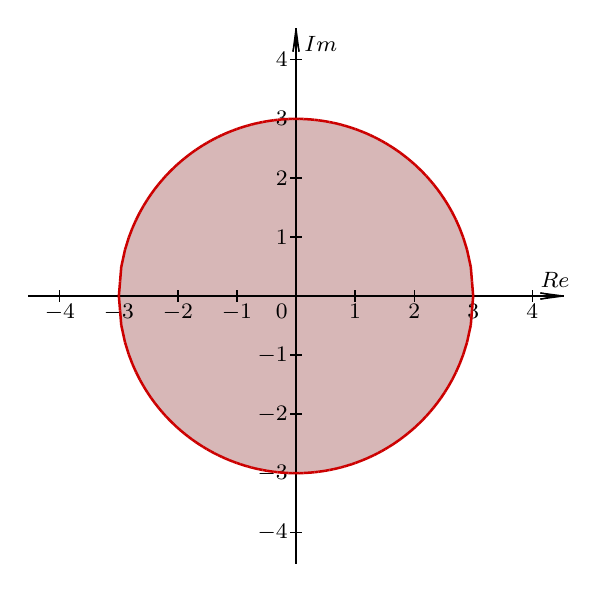
\begin{tikzpicture}
                    % \clip (0,0) rectangle (14.000000,10.000000);
                    {\footnotesize

                    % Changing color 215 183 183
                    \definecolor{r215g183b183}{rgb}{0.843137,0.717647,0.717647}%
                    \color{r215g183b183}% 

                    % Filling circle S A
                    \fill (4.100000,4.000000) circle (2.250000);%

                    % Changing color 0 0 0
                    \definecolor{r0g0b0}{rgb}{0.000000,0.000000,0.000000}%
                    \color{r0g0b0}% 

                    % Drawing 2D Cartesian system
                    \draw (4.100000,4.000000) node [anchor=north east] { $0$ };%
                    \draw [line width=0.016cm] (4.100000,3.925000) -- (4.100000,4.075000);%
                    \draw (4.850000,4.000000) node [anchor=north] { $1$ };%
                    \draw [line width=0.016cm] (4.850000,3.925000) -- (4.850000,4.075000);%
                    \draw (5.600000,4.000000) node [anchor=north] { $2$ };%
                    \draw [line width=0.016cm] (5.600000,3.925000) -- (5.600000,4.075000);%
                    \draw (6.350000,4.000000) node [anchor=north] { $3$ };%
                    \draw [line width=0.016cm] (6.350000,3.925000) -- (6.350000,4.075000);%
                    \draw (7.100000,4.000000) node [anchor=north] { $4$ };%
                    \draw [line width=0.016cm] (7.100000,3.925000) -- (7.100000,4.075000);%
                    \draw (3.350000,4.000000) node [anchor=north] { $-1$ };%
                    \draw [line width=0.016cm] (3.350000,3.925000) -- (3.350000,4.075000);%
                    \draw (2.600000,4.000000) node [anchor=north] { $-2$ };%
                    \draw [line width=0.016cm] (2.600000,3.925000) -- (2.600000,4.075000);%
                    \draw (1.850000,4.000000) node [anchor=north] { $-3$ };%
                    \draw [line width=0.016cm] (1.850000,3.925000) -- (1.850000,4.075000);%
                    \draw (1.100000,4.000000) node [anchor=north] { $-4$ };%
                    \draw [line width=0.016cm] (1.100000,3.925000) -- (1.100000,4.075000);%
                    \draw (4.100000,4.750000) node [anchor=east] { $1$ };%
                    \draw [line width=0.016cm] (4.025000,4.750000) -- (4.175000,4.750000);%
                    \draw (4.100000,5.500000) node [anchor=east] { $2$ };%
                    \draw [line width=0.016cm] (4.025000,5.500000) -- (4.175000,5.500000);%
                    \draw (4.100000,6.250000) node [anchor=east] { $3$ };%
                    \draw [line width=0.016cm] (4.025000,6.250000) -- (4.175000,6.250000);%
                    \draw (4.100000,7.000000) node [anchor=east] { $4$ };%
                    \draw [line width=0.016cm] (4.025000,7.000000) -- (4.175000,7.000000);%
                    \draw (4.100000,3.250000) node [anchor=east] { $-1$ };%
                    \draw [line width=0.016cm] (4.025000,3.250000) -- (4.175000,3.250000);%
                    \draw (4.100000,2.500000) node [anchor=east] { $-2$ };%
                    \draw [line width=0.016cm] (4.025000,2.500000) -- (4.175000,2.500000);%
                    \draw (4.100000,1.750000) node [anchor=east] { $-3$ };%
                    \draw [line width=0.016cm] (4.025000,1.750000) -- (4.175000,1.750000);%
                    \draw (4.100000,1.000000) node [anchor=east] { $-4$ };%
                    \draw [line width=0.016cm] (4.025000,1.000000) -- (4.175000,1.000000);%
                    \draw [line width=0.016cm] (0.700000,4.000000) -- (7.500000,4.000000);%
                    \draw [line width=0.016cm] (7.202567,4.039158) -- (7.500000,4.000000);%
                    \draw [line width=0.016cm] (7.202567,4.039158) -- (7.400000,4.000000);%
                    \draw [line width=0.016cm] (7.202567,3.960842) -- (7.500000,4.000000);%
                    \draw [line width=0.016cm] (7.202567,3.960842) -- (7.400000,4.000000);%
                    \draw [line width=0.016cm] (4.100000,0.600000) -- (4.100000,7.400000);%
                    \draw [line width=0.016cm] (4.060842,7.102567) -- (4.100000,7.400000);%
                    \draw [line width=0.016cm] (4.060842,7.102567) -- (4.100000,7.300000);%
                    \draw [line width=0.016cm] (4.139158,7.102567) -- (4.100000,7.400000);%
                    \draw [line width=0.016cm] (4.139158,7.102567) -- (4.100000,7.300000);%

                    % Marking point Im
                    \draw (4.100000,7.000000) node [anchor=south west] { $Im$ };%

                    % Marking point Re
                    \draw (7.100000,4.000000) node [anchor=south west] { $Re$ };%

                    % Changing color 204 0 0
                    \definecolor{r204g0b0}{rgb}{0.800000,0.000000,0.000000}%
                    \color{r204g0b0}% 

                    % Drawing 2D ang conic k
                    \draw [line width=0.032cm] (1.850000,4.000000) -- (1.865278,4.184774);%
                    \draw [line width=0.032cm] (1.865278,4.184774) -- (1.880556,4.369549);%
                    \draw [line width=0.032cm] (1.850000,4.000000) -- (1.865278,3.815226);%
                    \draw [line width=0.032cm] (1.865278,3.815226) -- (1.880556,3.630451);%
                    \draw [line width=0.032cm] (1.880556,4.369549) -- (1.927778,4.586473);%
                    \draw [line width=0.032cm] (1.880556,3.630451) -- (1.927778,3.413527);%
                    \draw [line width=0.032cm] (1.927778,4.586473) -- (1.975000,4.739510);%
                    \draw [line width=0.032cm] (1.927778,3.413527) -- (1.975000,3.260490);%
                    \draw [line width=0.032cm] (1.975000,4.739510) -- (2.022222,4.863330);%
                    \draw [line width=0.032cm] (1.975000,3.260490) -- (2.022222,3.136670);%
                    \draw [line width=0.032cm] (2.022222,4.863330) -- (2.069444,4.969198);%
                    \draw [line width=0.032cm] (2.022222,3.136670) -- (2.069444,3.030802);%
                    \draw [line width=0.032cm] (2.069444,4.969198) -- (2.116667,5.062492);%
                    \draw [line width=0.032cm] (2.069444,3.030802) -- (2.116667,2.937508);%
                    \draw [line width=0.032cm] (2.116667,5.062492) -- (2.163889,5.146287);%
                    \draw [line width=0.032cm] (2.116667,2.937508) -- (2.163889,2.853713);%
                    \draw [line width=0.032cm] (2.163889,5.146287) -- (2.211111,5.222538);%
                    \draw [line width=0.032cm] (2.163889,2.853713) -- (2.211111,2.777462);%
                    \draw [line width=0.032cm] (2.211111,5.222538) -- (2.258333,5.292580);%
                    \draw [line width=0.032cm] (2.211111,2.777462) -- (2.258333,2.707420);%
                    \draw [line width=0.032cm] (2.258333,5.292580) -- (2.305556,5.357376);%
                    \draw [line width=0.032cm] (2.258333,2.707420) -- (2.305556,2.642624);%
                    \draw [line width=0.032cm] (2.305556,5.357376) -- (2.352778,5.417644);%
                    \draw [line width=0.032cm] (2.305556,2.642624) -- (2.352778,2.582356);%
                    \draw [line width=0.032cm] (2.352778,5.417644) -- (2.400000,5.473940);%
                    \draw [line width=0.032cm] (2.352778,2.582356) -- (2.400000,2.526060);%
                    \draw [line width=0.032cm] (2.400000,5.473940) -- (2.447222,5.526704);%
                    \draw [line width=0.032cm] (2.400000,2.526060) -- (2.447222,2.473296);%
                    \draw [line width=0.032cm] (2.447222,5.526704) -- (2.494444,5.576290);%
                    \draw [line width=0.032cm] (2.447222,2.473296) -- (2.494444,2.423710);%
                    \draw [line width=0.032cm] (2.494444,5.576290) -- (2.541667,5.622990);%
                    \draw [line width=0.032cm] (2.494444,2.423710) -- (2.541667,2.377010);%
                    \draw [line width=0.032cm] (2.541667,5.622990) -- (2.588889,5.667046);%
                    \draw [line width=0.032cm] (2.541667,2.377010) -- (2.588889,2.332954);%
                    \draw [line width=0.032cm] (2.588889,5.667046) -- (2.636111,5.708663);%
                    \draw [line width=0.032cm] (2.588889,2.332954) -- (2.636111,2.291337);%
                    \draw [line width=0.032cm] (2.636111,5.708663) -- (2.683333,5.748015);%
                    \draw [line width=0.032cm] (2.636111,2.291337) -- (2.683333,2.251985);%
                    \draw [line width=0.032cm] (2.683333,5.748015) -- (2.730556,5.785251);%
                    \draw [line width=0.032cm] (2.683333,2.251985) -- (2.730556,2.214749);%
                    \draw [line width=0.032cm] (2.730556,5.785251) -- (2.777778,5.820502);%
                    \draw [line width=0.032cm] (2.730556,2.214749) -- (2.777778,2.179498);%
                    \draw [line width=0.032cm] (2.777778,5.820502) -- (2.825000,5.853881);%
                    \draw [line width=0.032cm] (2.777778,2.179498) -- (2.825000,2.146119);%
                    \draw [line width=0.032cm] (2.825000,5.853881) -- (2.872222,5.885487);%
                    \draw [line width=0.032cm] (2.825000,2.146119) -- (2.872222,2.114513);%
                    \draw [line width=0.032cm] (2.872222,5.885487) -- (2.919444,5.915408);%
                    \draw [line width=0.032cm] (2.872222,2.114513) -- (2.919444,2.084592);%
                    \draw [line width=0.032cm] (2.919444,5.915408) -- (2.966667,5.943722);%
                    \draw [line width=0.032cm] (2.919444,2.084592) -- (2.966667,2.056278);%
                    \draw [line width=0.032cm] (2.966667,5.943722) -- (3.013889,5.970498);%
                    \draw [line width=0.032cm] (2.966667,2.056278) -- (3.013889,2.029502);%
                    \draw [line width=0.032cm] (3.013889,5.970498) -- (3.061111,5.995798);%
                    \draw [line width=0.032cm] (3.013889,2.029502) -- (3.061111,2.004202);%
                    \draw [line width=0.032cm] (3.061111,5.995798) -- (3.108333,6.019678);%
                    \draw [line width=0.032cm] (3.061111,2.004202) -- (3.108333,1.980322);%
                    \draw [line width=0.032cm] (3.108333,6.019678) -- (3.155556,6.042186);%
                    \draw [line width=0.032cm] (3.108333,1.980322) -- (3.155556,1.957814);%
                    \draw [line width=0.032cm] (3.155556,6.042186) -- (3.202778,6.063369);%
                    \draw [line width=0.032cm] (3.155556,1.957814) -- (3.202778,1.936631);%
                    \draw [line width=0.032cm] (3.202778,6.063369) -- (3.250000,6.083267);%
                    \draw [line width=0.032cm] (3.202778,1.936631) -- (3.250000,1.916733);%
                    \draw [line width=0.032cm] (3.250000,6.083267) -- (3.297222,6.101915);%
                    \draw [line width=0.032cm] (3.250000,1.916733) -- (3.297222,1.898085);%
                    \draw [line width=0.032cm] (3.297222,6.101915) -- (3.344444,6.119348);%
                    \draw [line width=0.032cm] (3.297222,1.898085) -- (3.344444,1.880652);%
                    \draw [line width=0.032cm] (3.344444,6.119348) -- (3.391667,6.135595);%
                    \draw [line width=0.032cm] (3.344444,1.880652) -- (3.391667,1.864405);%
                    \draw [line width=0.032cm] (3.391667,6.135595) -- (3.438889,6.150682);%
                    \draw [line width=0.032cm] (3.391667,1.864405) -- (3.438889,1.849318);%
                    \draw [line width=0.032cm] (3.438889,6.150682) -- (3.486111,6.164634);%
                    \draw [line width=0.032cm] (3.438889,1.849318) -- (3.486111,1.835366);%
                    \draw [line width=0.032cm] (3.486111,6.164634) -- (3.533333,6.177473);%
                    \draw [line width=0.032cm] (3.486111,1.835366) -- (3.533333,1.822527);%
                    \draw [line width=0.032cm] (3.533333,6.177473) -- (3.580556,6.189218);%
                    \draw [line width=0.032cm] (3.533333,1.822527) -- (3.580556,1.810782);%
                    \draw [line width=0.032cm] (3.580556,6.189218) -- (3.627778,6.199888);%
                    \draw [line width=0.032cm] (3.580556,1.810782) -- (3.627778,1.800112);%
                    \draw [line width=0.032cm] (3.627778,6.199888) -- (3.675000,6.209497);%
                    \draw [line width=0.032cm] (3.627778,1.800112) -- (3.675000,1.790503);%
                    \draw [line width=0.032cm] (3.675000,6.209497) -- (3.722222,6.218059);%
                    \draw [line width=0.032cm] (3.675000,1.790503) -- (3.722222,1.781941);%
                    \draw [line width=0.032cm] (3.722222,6.218059) -- (3.769444,6.225586);%
                    \draw [line width=0.032cm] (3.722222,1.781941) -- (3.769444,1.774414);%
                    \draw [line width=0.032cm] (3.769444,6.225586) -- (3.816667,6.232089);%
                    \draw [line width=0.032cm] (3.769444,1.774414) -- (3.816667,1.767911);%
                    \draw [line width=0.032cm] (3.816667,6.232089) -- (3.863889,6.237577);%
                    \draw [line width=0.032cm] (3.816667,1.767911) -- (3.863889,1.762423);%
                    \draw [line width=0.032cm] (3.863889,6.237577) -- (3.911111,6.242057);%
                    \draw [line width=0.032cm] (3.863889,1.762423) -- (3.911111,1.757943);%
                    \draw [line width=0.032cm] (3.911111,6.242057) -- (3.958333,6.245536);%
                    \draw [line width=0.032cm] (3.911111,1.757943) -- (3.958333,1.754464);%
                    \draw [line width=0.032cm] (3.958333,6.245536) -- (4.005556,6.248017);%
                    \draw [line width=0.032cm] (3.958333,1.754464) -- (4.005556,1.751983);%
                    \draw [line width=0.032cm] (4.005556,6.248017) -- (4.052778,6.249504);%
                    \draw [line width=0.032cm] (4.005556,1.751983) -- (4.052778,1.750496);%
                    \draw [line width=0.032cm] (4.052778,6.249504) -- (4.100000,6.250000);%
                    \draw [line width=0.032cm] (4.052778,1.750496) -- (4.100000,1.750000);%
                    \draw [line width=0.032cm] (4.100000,6.250000) -- (4.147222,6.249504);%
                    \draw [line width=0.032cm] (4.100000,1.750000) -- (4.147222,1.750496);%
                    \draw [line width=0.032cm] (4.147222,6.249504) -- (4.194444,6.248017);%
                    \draw [line width=0.032cm] (4.147222,1.750496) -- (4.194444,1.751983);%
                    \draw [line width=0.032cm] (4.194444,6.248017) -- (4.241667,6.245536);%
                    \draw [line width=0.032cm] (4.194444,1.751983) -- (4.241667,1.754464);%
                    \draw [line width=0.032cm] (4.241667,6.245536) -- (4.288889,6.242057);%
                    \draw [line width=0.032cm] (4.241667,1.754464) -- (4.288889,1.757943);%
                    \draw [line width=0.032cm] (4.288889,6.242057) -- (4.336111,6.237577);%
                    \draw [line width=0.032cm] (4.288889,1.757943) -- (4.336111,1.762423);%
                    \draw [line width=0.032cm] (4.336111,6.237577) -- (4.383333,6.232089);%
                    \draw [line width=0.032cm] (4.336111,1.762423) -- (4.383333,1.767911);%
                    \draw [line width=0.032cm] (4.383333,6.232089) -- (4.430556,6.225586);%
                    \draw [line width=0.032cm] (4.383333,1.767911) -- (4.430556,1.774414);%
                    \draw [line width=0.032cm] (4.430556,6.225586) -- (4.477778,6.218059);%
                    \draw [line width=0.032cm] (4.430556,1.774414) -- (4.477778,1.781941);%
                    \draw [line width=0.032cm] (4.477778,6.218059) -- (4.525000,6.209497);%
                    \draw [line width=0.032cm] (4.477778,1.781941) -- (4.525000,1.790503);%
                    \draw [line width=0.032cm] (4.525000,6.209497) -- (4.572222,6.199888);%
                    \draw [line width=0.032cm] (4.525000,1.790503) -- (4.572222,1.800112);%
                    \draw [line width=0.032cm] (4.572222,6.199888) -- (4.619444,6.189218);%
                    \draw [line width=0.032cm] (4.572222,1.800112) -- (4.619444,1.810782);%
                    \draw [line width=0.032cm] (4.619444,6.189218) -- (4.666667,6.177473);%
                    \draw [line width=0.032cm] (4.619444,1.810782) -- (4.666667,1.822527);%
                    \draw [line width=0.032cm] (4.666667,6.177473) -- (4.713889,6.164634);%
                    \draw [line width=0.032cm] (4.666667,1.822527) -- (4.713889,1.835366);%
                    \draw [line width=0.032cm] (4.713889,6.164634) -- (4.761111,6.150682);%
                    \draw [line width=0.032cm] (4.713889,1.835366) -- (4.761111,1.849318);%
                    \draw [line width=0.032cm] (4.761111,6.150682) -- (4.808333,6.135595);%
                    \draw [line width=0.032cm] (4.761111,1.849318) -- (4.808333,1.864405);%
                    \draw [line width=0.032cm] (4.808333,6.135595) -- (4.855556,6.119348);%
                    \draw [line width=0.032cm] (4.808333,1.864405) -- (4.855556,1.880652);%
                    \draw [line width=0.032cm] (4.855556,6.119348) -- (4.902778,6.101915);%
                    \draw [line width=0.032cm] (4.855556,1.880652) -- (4.902778,1.898085);%
                    \draw [line width=0.032cm] (4.902778,6.101915) -- (4.950000,6.083267);%
                    \draw [line width=0.032cm] (4.902778,1.898085) -- (4.950000,1.916733);%
                    \draw [line width=0.032cm] (4.950000,6.083267) -- (4.997222,6.063369);%
                    \draw [line width=0.032cm] (4.950000,1.916733) -- (4.997222,1.936631);%
                    \draw [line width=0.032cm] (4.997222,6.063369) -- (5.044444,6.042186);%
                    \draw [line width=0.032cm] (4.997222,1.936631) -- (5.044444,1.957814);%
                    \draw [line width=0.032cm] (5.044444,6.042186) -- (5.091667,6.019678);%
                    \draw [line width=0.032cm] (5.044444,1.957814) -- (5.091667,1.980322);%
                    \draw [line width=0.032cm] (5.091667,6.019678) -- (5.138889,5.995798);%
                    \draw [line width=0.032cm] (5.091667,1.980322) -- (5.138889,2.004202);%
                    \draw [line width=0.032cm] (5.138889,5.995798) -- (5.186111,5.970498);%
                    \draw [line width=0.032cm] (5.138889,2.004202) -- (5.186111,2.029502);%
                    \draw [line width=0.032cm] (5.186111,5.970498) -- (5.233333,5.943722);%
                    \draw [line width=0.032cm] (5.186111,2.029502) -- (5.233333,2.056278);%
                    \draw [line width=0.032cm] (5.233333,5.943722) -- (5.280556,5.915408);%
                    \draw [line width=0.032cm] (5.233333,2.056278) -- (5.280556,2.084592);%
                    \draw [line width=0.032cm] (5.280556,5.915408) -- (5.327778,5.885487);%
                    \draw [line width=0.032cm] (5.280556,2.084592) -- (5.327778,2.114513);%
                    \draw [line width=0.032cm] (5.327778,5.885487) -- (5.375000,5.853881);%
                    \draw [line width=0.032cm] (5.327778,2.114513) -- (5.375000,2.146119);%
                    \draw [line width=0.032cm] (5.375000,5.853881) -- (5.422222,5.820502);%
                    \draw [line width=0.032cm] (5.375000,2.146119) -- (5.422222,2.179498);%
                    \draw [line width=0.032cm] (5.422222,5.820502) -- (5.469444,5.785251);%
                    \draw [line width=0.032cm] (5.422222,2.179498) -- (5.469444,2.214749);%
                    \draw [line width=0.032cm] (5.469444,5.785251) -- (5.516667,5.748015);%
                    \draw [line width=0.032cm] (5.469444,2.214749) -- (5.516667,2.251985);%
                    \draw [line width=0.032cm] (5.516667,5.748015) -- (5.563889,5.708663);%
                    \draw [line width=0.032cm] (5.516667,2.251985) -- (5.563889,2.291337);%
                    \draw [line width=0.032cm] (5.563889,5.708663) -- (5.611111,5.667046);%
                    \draw [line width=0.032cm] (5.563889,2.291337) -- (5.611111,2.332954);%
                    \draw [line width=0.032cm] (5.611111,5.667046) -- (5.658333,5.622990);%
                    \draw [line width=0.032cm] (5.611111,2.332954) -- (5.658333,2.377010);%
                    \draw [line width=0.032cm] (5.658333,5.622990) -- (5.705556,5.576290);%
                    \draw [line width=0.032cm] (5.658333,2.377010) -- (5.705556,2.423710);%
                    \draw [line width=0.032cm] (5.705556,5.576290) -- (5.752778,5.526704);%
                    \draw [line width=0.032cm] (5.705556,2.423710) -- (5.752778,2.473296);%
                    \draw [line width=0.032cm] (5.752778,5.526704) -- (5.800000,5.473940);%
                    \draw [line width=0.032cm] (5.752778,2.473296) -- (5.800000,2.526060);%
                    \draw [line width=0.032cm] (5.800000,5.473940) -- (5.847222,5.417644);%
                    \draw [line width=0.032cm] (5.800000,2.526060) -- (5.847222,2.582356);%
                    \draw [line width=0.032cm] (5.847222,5.417644) -- (5.894444,5.357376);%
                    \draw [line width=0.032cm] (5.847222,2.582356) -- (5.894444,2.642624);%
                    \draw [line width=0.032cm] (5.894444,5.357376) -- (5.941667,5.292580);%
                    \draw [line width=0.032cm] (5.894444,2.642624) -- (5.941667,2.707420);%
                    \draw [line width=0.032cm] (5.941667,5.292580) -- (5.988889,5.222538);%
                    \draw [line width=0.032cm] (5.941667,2.707420) -- (5.988889,2.777462);%
                    \draw [line width=0.032cm] (5.988889,5.222538) -- (6.036111,5.146287);%
                    \draw [line width=0.032cm] (5.988889,2.777462) -- (6.036111,2.853713);%
                    \draw [line width=0.032cm] (6.036111,5.146287) -- (6.083333,5.062492);%
                    \draw [line width=0.032cm] (6.036111,2.853713) -- (6.083333,2.937508);%
                    \draw [line width=0.032cm] (6.083333,5.062492) -- (6.130556,4.969198);%
                    \draw [line width=0.032cm] (6.083333,2.937508) -- (6.130556,3.030802);%
                    \draw [line width=0.032cm] (6.130556,4.969198) -- (6.177778,4.863330);%
                    \draw [line width=0.032cm] (6.130556,3.030802) -- (6.177778,3.136670);%
                    \draw [line width=0.032cm] (6.177778,4.863330) -- (6.225000,4.739510);%
                    \draw [line width=0.032cm] (6.177778,3.136670) -- (6.225000,3.260490);%
                    \draw [line width=0.032cm] (6.225000,4.739510) -- (6.272222,4.586473);%
                    \draw [line width=0.032cm] (6.225000,3.260490) -- (6.272222,3.413527);%
                    \draw [line width=0.032cm] (6.272222,4.586473) -- (6.319444,4.369549);%
                    \draw [line width=0.032cm] (6.272222,3.413527) -- (6.319444,3.630451);%
                    \draw [line width=0.032cm] (6.350000,4.000000) -- (6.334722,4.184774);%
                    \draw [line width=0.032cm] (6.334722,4.184774) -- (6.319444,4.369549);%
                    \draw [line width=0.032cm] (6.350000,4.000000) -- (6.334722,3.815226);%
                    \draw [line width=0.032cm] (6.334722,3.815226) -- (6.319444,3.630451);%
                    \color{black}
                    }
                    \end{tikzpicture}

                \end{figure}
                
            \end{exampleblock}}


        \end{frame}

        \begin{frame}

            \only<2->{\begin{exampleblock}{Naloga}
                Za označeno množico točk zapišite, katermu pogoju ustreza.
                \vskip-1em
                \begin{figure}[H]
                    \centering
                    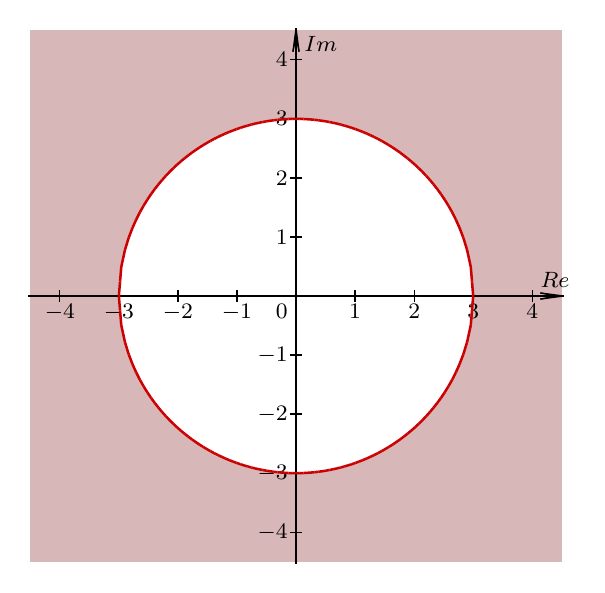
\begin{tikzpicture}
                    % \clip (0,0) rectangle (14.000000,10.000000);
                    {\footnotesize

                    % Changing color 215 183 183
                    \definecolor{r215g183b183}{rgb}{0.843137,0.717647,0.717647}%
                    \color{r215g183b183}% 

                    % Filling rectangle left-bottom: B right-top: C
                    \fill (0.725000,0.625000) -- (7.475000,0.625000) -- (7.475000,7.375000) -- (0.725000,7.375000);%

                    % Changing color 255 255 255
                    \definecolor{r255g255b255}{rgb}{1.000000,1.000000,1.000000}%
                    \color{r255g255b255}% 

                    % Filling circle S A
                    \fill (4.100000,4.000000) circle (2.250000);%

                    % Changing color 0 0 0
                    \definecolor{r0g0b0}{rgb}{0.000000,0.000000,0.000000}%
                    \color{r0g0b0}% 

                    % Drawing 2D Cartesian system
                    \draw (4.100000,4.000000) node [anchor=north east] { $0$ };%
                    \draw [line width=0.016cm] (4.100000,3.925000) -- (4.100000,4.075000);%
                    \draw (4.850000,4.000000) node [anchor=north] { $1$ };%
                    \draw [line width=0.016cm] (4.850000,3.925000) -- (4.850000,4.075000);%
                    \draw (5.600000,4.000000) node [anchor=north] { $2$ };%
                    \draw [line width=0.016cm] (5.600000,3.925000) -- (5.600000,4.075000);%
                    \draw (6.350000,4.000000) node [anchor=north] { $3$ };%
                    \draw [line width=0.016cm] (6.350000,3.925000) -- (6.350000,4.075000);%
                    \draw (7.100000,4.000000) node [anchor=north] { $4$ };%
                    \draw [line width=0.016cm] (7.100000,3.925000) -- (7.100000,4.075000);%
                    \draw (3.350000,4.000000) node [anchor=north] { $-1$ };%
                    \draw [line width=0.016cm] (3.350000,3.925000) -- (3.350000,4.075000);%
                    \draw (2.600000,4.000000) node [anchor=north] { $-2$ };%
                    \draw [line width=0.016cm] (2.600000,3.925000) -- (2.600000,4.075000);%
                    \draw (1.850000,4.000000) node [anchor=north] { $-3$ };%
                    \draw [line width=0.016cm] (1.850000,3.925000) -- (1.850000,4.075000);%
                    \draw (1.100000,4.000000) node [anchor=north] { $-4$ };%
                    \draw [line width=0.016cm] (1.100000,3.925000) -- (1.100000,4.075000);%
                    \draw (4.100000,4.750000) node [anchor=east] { $1$ };%
                    \draw [line width=0.016cm] (4.025000,4.750000) -- (4.175000,4.750000);%
                    \draw (4.100000,5.500000) node [anchor=east] { $2$ };%
                    \draw [line width=0.016cm] (4.025000,5.500000) -- (4.175000,5.500000);%
                    \draw (4.100000,6.250000) node [anchor=east] { $3$ };%
                    \draw [line width=0.016cm] (4.025000,6.250000) -- (4.175000,6.250000);%
                    \draw (4.100000,7.000000) node [anchor=east] { $4$ };%
                    \draw [line width=0.016cm] (4.025000,7.000000) -- (4.175000,7.000000);%
                    \draw (4.100000,3.250000) node [anchor=east] { $-1$ };%
                    \draw [line width=0.016cm] (4.025000,3.250000) -- (4.175000,3.250000);%
                    \draw (4.100000,2.500000) node [anchor=east] { $-2$ };%
                    \draw [line width=0.016cm] (4.025000,2.500000) -- (4.175000,2.500000);%
                    \draw (4.100000,1.750000) node [anchor=east] { $-3$ };%
                    \draw [line width=0.016cm] (4.025000,1.750000) -- (4.175000,1.750000);%
                    \draw (4.100000,1.000000) node [anchor=east] { $-4$ };%
                    \draw [line width=0.016cm] (4.025000,1.000000) -- (4.175000,1.000000);%
                    \draw [line width=0.016cm] (0.700000,4.000000) -- (7.500000,4.000000);%
                    \draw [line width=0.016cm] (7.202567,4.039158) -- (7.500000,4.000000);%
                    \draw [line width=0.016cm] (7.202567,4.039158) -- (7.400000,4.000000);%
                    \draw [line width=0.016cm] (7.202567,3.960842) -- (7.500000,4.000000);%
                    \draw [line width=0.016cm] (7.202567,3.960842) -- (7.400000,4.000000);%
                    \draw [line width=0.016cm] (4.100000,0.600000) -- (4.100000,7.400000);%
                    \draw [line width=0.016cm] (4.060842,7.102567) -- (4.100000,7.400000);%
                    \draw [line width=0.016cm] (4.060842,7.102567) -- (4.100000,7.300000);%
                    \draw [line width=0.016cm] (4.139158,7.102567) -- (4.100000,7.400000);%
                    \draw [line width=0.016cm] (4.139158,7.102567) -- (4.100000,7.300000);%

                    % Marking point Im
                    \draw (4.100000,7.000000) node [anchor=south west] { $Im$ };%

                    % Marking point Re
                    \draw (7.100000,4.000000) node [anchor=south west] { $Re$ };%

                    % Changing color 204 0 0
                    \definecolor{r204g0b0}{rgb}{0.800000,0.000000,0.000000}%
                    \color{r204g0b0}% 

                    % Drawing 2D ang conic k
                    \draw [line width=0.032cm] (1.850000,4.000000) -- (1.865278,4.184774);%
                    \draw [line width=0.032cm] (1.865278,4.184774) -- (1.880556,4.369549);%
                    \draw [line width=0.032cm] (1.850000,4.000000) -- (1.865278,3.815226);%
                    \draw [line width=0.032cm] (1.865278,3.815226) -- (1.880556,3.630451);%
                    \draw [line width=0.032cm] (1.880556,4.369549) -- (1.927778,4.586473);%
                    \draw [line width=0.032cm] (1.880556,3.630451) -- (1.927778,3.413527);%
                    \draw [line width=0.032cm] (1.927778,4.586473) -- (1.975000,4.739510);%
                    \draw [line width=0.032cm] (1.927778,3.413527) -- (1.975000,3.260490);%
                    \draw [line width=0.032cm] (1.975000,4.739510) -- (2.022222,4.863330);%
                    \draw [line width=0.032cm] (1.975000,3.260490) -- (2.022222,3.136670);%
                    \draw [line width=0.032cm] (2.022222,4.863330) -- (2.069444,4.969198);%
                    \draw [line width=0.032cm] (2.022222,3.136670) -- (2.069444,3.030802);%
                    \draw [line width=0.032cm] (2.069444,4.969198) -- (2.116667,5.062492);%
                    \draw [line width=0.032cm] (2.069444,3.030802) -- (2.116667,2.937508);%
                    \draw [line width=0.032cm] (2.116667,5.062492) -- (2.163889,5.146287);%
                    \draw [line width=0.032cm] (2.116667,2.937508) -- (2.163889,2.853713);%
                    \draw [line width=0.032cm] (2.163889,5.146287) -- (2.211111,5.222538);%
                    \draw [line width=0.032cm] (2.163889,2.853713) -- (2.211111,2.777462);%
                    \draw [line width=0.032cm] (2.211111,5.222538) -- (2.258333,5.292580);%
                    \draw [line width=0.032cm] (2.211111,2.777462) -- (2.258333,2.707420);%
                    \draw [line width=0.032cm] (2.258333,5.292580) -- (2.305556,5.357376);%
                    \draw [line width=0.032cm] (2.258333,2.707420) -- (2.305556,2.642624);%
                    \draw [line width=0.032cm] (2.305556,5.357376) -- (2.352778,5.417644);%
                    \draw [line width=0.032cm] (2.305556,2.642624) -- (2.352778,2.582356);%
                    \draw [line width=0.032cm] (2.352778,5.417644) -- (2.400000,5.473940);%
                    \draw [line width=0.032cm] (2.352778,2.582356) -- (2.400000,2.526060);%
                    \draw [line width=0.032cm] (2.400000,5.473940) -- (2.447222,5.526704);%
                    \draw [line width=0.032cm] (2.400000,2.526060) -- (2.447222,2.473296);%
                    \draw [line width=0.032cm] (2.447222,5.526704) -- (2.494444,5.576290);%
                    \draw [line width=0.032cm] (2.447222,2.473296) -- (2.494444,2.423710);%
                    \draw [line width=0.032cm] (2.494444,5.576290) -- (2.541667,5.622990);%
                    \draw [line width=0.032cm] (2.494444,2.423710) -- (2.541667,2.377010);%
                    \draw [line width=0.032cm] (2.541667,5.622990) -- (2.588889,5.667046);%
                    \draw [line width=0.032cm] (2.541667,2.377010) -- (2.588889,2.332954);%
                    \draw [line width=0.032cm] (2.588889,5.667046) -- (2.636111,5.708663);%
                    \draw [line width=0.032cm] (2.588889,2.332954) -- (2.636111,2.291337);%
                    \draw [line width=0.032cm] (2.636111,5.708663) -- (2.683333,5.748015);%
                    \draw [line width=0.032cm] (2.636111,2.291337) -- (2.683333,2.251985);%
                    \draw [line width=0.032cm] (2.683333,5.748015) -- (2.730556,5.785251);%
                    \draw [line width=0.032cm] (2.683333,2.251985) -- (2.730556,2.214749);%
                    \draw [line width=0.032cm] (2.730556,5.785251) -- (2.777778,5.820502);%
                    \draw [line width=0.032cm] (2.730556,2.214749) -- (2.777778,2.179498);%
                    \draw [line width=0.032cm] (2.777778,5.820502) -- (2.825000,5.853881);%
                    \draw [line width=0.032cm] (2.777778,2.179498) -- (2.825000,2.146119);%
                    \draw [line width=0.032cm] (2.825000,5.853881) -- (2.872222,5.885487);%
                    \draw [line width=0.032cm] (2.825000,2.146119) -- (2.872222,2.114513);%
                    \draw [line width=0.032cm] (2.872222,5.885487) -- (2.919444,5.915408);%
                    \draw [line width=0.032cm] (2.872222,2.114513) -- (2.919444,2.084592);%
                    \draw [line width=0.032cm] (2.919444,5.915408) -- (2.966667,5.943722);%
                    \draw [line width=0.032cm] (2.919444,2.084592) -- (2.966667,2.056278);%
                    \draw [line width=0.032cm] (2.966667,5.943722) -- (3.013889,5.970498);%
                    \draw [line width=0.032cm] (2.966667,2.056278) -- (3.013889,2.029502);%
                    \draw [line width=0.032cm] (3.013889,5.970498) -- (3.061111,5.995798);%
                    \draw [line width=0.032cm] (3.013889,2.029502) -- (3.061111,2.004202);%
                    \draw [line width=0.032cm] (3.061111,5.995798) -- (3.108333,6.019678);%
                    \draw [line width=0.032cm] (3.061111,2.004202) -- (3.108333,1.980322);%
                    \draw [line width=0.032cm] (3.108333,6.019678) -- (3.155556,6.042186);%
                    \draw [line width=0.032cm] (3.108333,1.980322) -- (3.155556,1.957814);%
                    \draw [line width=0.032cm] (3.155556,6.042186) -- (3.202778,6.063369);%
                    \draw [line width=0.032cm] (3.155556,1.957814) -- (3.202778,1.936631);%
                    \draw [line width=0.032cm] (3.202778,6.063369) -- (3.250000,6.083267);%
                    \draw [line width=0.032cm] (3.202778,1.936631) -- (3.250000,1.916733);%
                    \draw [line width=0.032cm] (3.250000,6.083267) -- (3.297222,6.101915);%
                    \draw [line width=0.032cm] (3.250000,1.916733) -- (3.297222,1.898085);%
                    \draw [line width=0.032cm] (3.297222,6.101915) -- (3.344444,6.119348);%
                    \draw [line width=0.032cm] (3.297222,1.898085) -- (3.344444,1.880652);%
                    \draw [line width=0.032cm] (3.344444,6.119348) -- (3.391667,6.135595);%
                    \draw [line width=0.032cm] (3.344444,1.880652) -- (3.391667,1.864405);%
                    \draw [line width=0.032cm] (3.391667,6.135595) -- (3.438889,6.150682);%
                    \draw [line width=0.032cm] (3.391667,1.864405) -- (3.438889,1.849318);%
                    \draw [line width=0.032cm] (3.438889,6.150682) -- (3.486111,6.164634);%
                    \draw [line width=0.032cm] (3.438889,1.849318) -- (3.486111,1.835366);%
                    \draw [line width=0.032cm] (3.486111,6.164634) -- (3.533333,6.177473);%
                    \draw [line width=0.032cm] (3.486111,1.835366) -- (3.533333,1.822527);%
                    \draw [line width=0.032cm] (3.533333,6.177473) -- (3.580556,6.189218);%
                    \draw [line width=0.032cm] (3.533333,1.822527) -- (3.580556,1.810782);%
                    \draw [line width=0.032cm] (3.580556,6.189218) -- (3.627778,6.199888);%
                    \draw [line width=0.032cm] (3.580556,1.810782) -- (3.627778,1.800112);%
                    \draw [line width=0.032cm] (3.627778,6.199888) -- (3.675000,6.209497);%
                    \draw [line width=0.032cm] (3.627778,1.800112) -- (3.675000,1.790503);%
                    \draw [line width=0.032cm] (3.675000,6.209497) -- (3.722222,6.218059);%
                    \draw [line width=0.032cm] (3.675000,1.790503) -- (3.722222,1.781941);%
                    \draw [line width=0.032cm] (3.722222,6.218059) -- (3.769444,6.225586);%
                    \draw [line width=0.032cm] (3.722222,1.781941) -- (3.769444,1.774414);%
                    \draw [line width=0.032cm] (3.769444,6.225586) -- (3.816667,6.232089);%
                    \draw [line width=0.032cm] (3.769444,1.774414) -- (3.816667,1.767911);%
                    \draw [line width=0.032cm] (3.816667,6.232089) -- (3.863889,6.237577);%
                    \draw [line width=0.032cm] (3.816667,1.767911) -- (3.863889,1.762423);%
                    \draw [line width=0.032cm] (3.863889,6.237577) -- (3.911111,6.242057);%
                    \draw [line width=0.032cm] (3.863889,1.762423) -- (3.911111,1.757943);%
                    \draw [line width=0.032cm] (3.911111,6.242057) -- (3.958333,6.245536);%
                    \draw [line width=0.032cm] (3.911111,1.757943) -- (3.958333,1.754464);%
                    \draw [line width=0.032cm] (3.958333,6.245536) -- (4.005556,6.248017);%
                    \draw [line width=0.032cm] (3.958333,1.754464) -- (4.005556,1.751983);%
                    \draw [line width=0.032cm] (4.005556,6.248017) -- (4.052778,6.249504);%
                    \draw [line width=0.032cm] (4.005556,1.751983) -- (4.052778,1.750496);%
                    \draw [line width=0.032cm] (4.052778,6.249504) -- (4.100000,6.250000);%
                    \draw [line width=0.032cm] (4.052778,1.750496) -- (4.100000,1.750000);%
                    \draw [line width=0.032cm] (4.100000,6.250000) -- (4.147222,6.249504);%
                    \draw [line width=0.032cm] (4.100000,1.750000) -- (4.147222,1.750496);%
                    \draw [line width=0.032cm] (4.147222,6.249504) -- (4.194444,6.248017);%
                    \draw [line width=0.032cm] (4.147222,1.750496) -- (4.194444,1.751983);%
                    \draw [line width=0.032cm] (4.194444,6.248017) -- (4.241667,6.245536);%
                    \draw [line width=0.032cm] (4.194444,1.751983) -- (4.241667,1.754464);%
                    \draw [line width=0.032cm] (4.241667,6.245536) -- (4.288889,6.242057);%
                    \draw [line width=0.032cm] (4.241667,1.754464) -- (4.288889,1.757943);%
                    \draw [line width=0.032cm] (4.288889,6.242057) -- (4.336111,6.237577);%
                    \draw [line width=0.032cm] (4.288889,1.757943) -- (4.336111,1.762423);%
                    \draw [line width=0.032cm] (4.336111,6.237577) -- (4.383333,6.232089);%
                    \draw [line width=0.032cm] (4.336111,1.762423) -- (4.383333,1.767911);%
                    \draw [line width=0.032cm] (4.383333,6.232089) -- (4.430556,6.225586);%
                    \draw [line width=0.032cm] (4.383333,1.767911) -- (4.430556,1.774414);%
                    \draw [line width=0.032cm] (4.430556,6.225586) -- (4.477778,6.218059);%
                    \draw [line width=0.032cm] (4.430556,1.774414) -- (4.477778,1.781941);%
                    \draw [line width=0.032cm] (4.477778,6.218059) -- (4.525000,6.209497);%
                    \draw [line width=0.032cm] (4.477778,1.781941) -- (4.525000,1.790503);%
                    \draw [line width=0.032cm] (4.525000,6.209497) -- (4.572222,6.199888);%
                    \draw [line width=0.032cm] (4.525000,1.790503) -- (4.572222,1.800112);%
                    \draw [line width=0.032cm] (4.572222,6.199888) -- (4.619444,6.189218);%
                    \draw [line width=0.032cm] (4.572222,1.800112) -- (4.619444,1.810782);%
                    \draw [line width=0.032cm] (4.619444,6.189218) -- (4.666667,6.177473);%
                    \draw [line width=0.032cm] (4.619444,1.810782) -- (4.666667,1.822527);%
                    \draw [line width=0.032cm] (4.666667,6.177473) -- (4.713889,6.164634);%
                    \draw [line width=0.032cm] (4.666667,1.822527) -- (4.713889,1.835366);%
                    \draw [line width=0.032cm] (4.713889,6.164634) -- (4.761111,6.150682);%
                    \draw [line width=0.032cm] (4.713889,1.835366) -- (4.761111,1.849318);%
                    \draw [line width=0.032cm] (4.761111,6.150682) -- (4.808333,6.135595);%
                    \draw [line width=0.032cm] (4.761111,1.849318) -- (4.808333,1.864405);%
                    \draw [line width=0.032cm] (4.808333,6.135595) -- (4.855556,6.119348);%
                    \draw [line width=0.032cm] (4.808333,1.864405) -- (4.855556,1.880652);%
                    \draw [line width=0.032cm] (4.855556,6.119348) -- (4.902778,6.101915);%
                    \draw [line width=0.032cm] (4.855556,1.880652) -- (4.902778,1.898085);%
                    \draw [line width=0.032cm] (4.902778,6.101915) -- (4.950000,6.083267);%
                    \draw [line width=0.032cm] (4.902778,1.898085) -- (4.950000,1.916733);%
                    \draw [line width=0.032cm] (4.950000,6.083267) -- (4.997222,6.063369);%
                    \draw [line width=0.032cm] (4.950000,1.916733) -- (4.997222,1.936631);%
                    \draw [line width=0.032cm] (4.997222,6.063369) -- (5.044444,6.042186);%
                    \draw [line width=0.032cm] (4.997222,1.936631) -- (5.044444,1.957814);%
                    \draw [line width=0.032cm] (5.044444,6.042186) -- (5.091667,6.019678);%
                    \draw [line width=0.032cm] (5.044444,1.957814) -- (5.091667,1.980322);%
                    \draw [line width=0.032cm] (5.091667,6.019678) -- (5.138889,5.995798);%
                    \draw [line width=0.032cm] (5.091667,1.980322) -- (5.138889,2.004202);%
                    \draw [line width=0.032cm] (5.138889,5.995798) -- (5.186111,5.970498);%
                    \draw [line width=0.032cm] (5.138889,2.004202) -- (5.186111,2.029502);%
                    \draw [line width=0.032cm] (5.186111,5.970498) -- (5.233333,5.943722);%
                    \draw [line width=0.032cm] (5.186111,2.029502) -- (5.233333,2.056278);%
                    \draw [line width=0.032cm] (5.233333,5.943722) -- (5.280556,5.915408);%
                    \draw [line width=0.032cm] (5.233333,2.056278) -- (5.280556,2.084592);%
                    \draw [line width=0.032cm] (5.280556,5.915408) -- (5.327778,5.885487);%
                    \draw [line width=0.032cm] (5.280556,2.084592) -- (5.327778,2.114513);%
                    \draw [line width=0.032cm] (5.327778,5.885487) -- (5.375000,5.853881);%
                    \draw [line width=0.032cm] (5.327778,2.114513) -- (5.375000,2.146119);%
                    \draw [line width=0.032cm] (5.375000,5.853881) -- (5.422222,5.820502);%
                    \draw [line width=0.032cm] (5.375000,2.146119) -- (5.422222,2.179498);%
                    \draw [line width=0.032cm] (5.422222,5.820502) -- (5.469444,5.785251);%
                    \draw [line width=0.032cm] (5.422222,2.179498) -- (5.469444,2.214749);%
                    \draw [line width=0.032cm] (5.469444,5.785251) -- (5.516667,5.748015);%
                    \draw [line width=0.032cm] (5.469444,2.214749) -- (5.516667,2.251985);%
                    \draw [line width=0.032cm] (5.516667,5.748015) -- (5.563889,5.708663);%
                    \draw [line width=0.032cm] (5.516667,2.251985) -- (5.563889,2.291337);%
                    \draw [line width=0.032cm] (5.563889,5.708663) -- (5.611111,5.667046);%
                    \draw [line width=0.032cm] (5.563889,2.291337) -- (5.611111,2.332954);%
                    \draw [line width=0.032cm] (5.611111,5.667046) -- (5.658333,5.622990);%
                    \draw [line width=0.032cm] (5.611111,2.332954) -- (5.658333,2.377010);%
                    \draw [line width=0.032cm] (5.658333,5.622990) -- (5.705556,5.576290);%
                    \draw [line width=0.032cm] (5.658333,2.377010) -- (5.705556,2.423710);%
                    \draw [line width=0.032cm] (5.705556,5.576290) -- (5.752778,5.526704);%
                    \draw [line width=0.032cm] (5.705556,2.423710) -- (5.752778,2.473296);%
                    \draw [line width=0.032cm] (5.752778,5.526704) -- (5.800000,5.473940);%
                    \draw [line width=0.032cm] (5.752778,2.473296) -- (5.800000,2.526060);%
                    \draw [line width=0.032cm] (5.800000,5.473940) -- (5.847222,5.417644);%
                    \draw [line width=0.032cm] (5.800000,2.526060) -- (5.847222,2.582356);%
                    \draw [line width=0.032cm] (5.847222,5.417644) -- (5.894444,5.357376);%
                    \draw [line width=0.032cm] (5.847222,2.582356) -- (5.894444,2.642624);%
                    \draw [line width=0.032cm] (5.894444,5.357376) -- (5.941667,5.292580);%
                    \draw [line width=0.032cm] (5.894444,2.642624) -- (5.941667,2.707420);%
                    \draw [line width=0.032cm] (5.941667,5.292580) -- (5.988889,5.222538);%
                    \draw [line width=0.032cm] (5.941667,2.707420) -- (5.988889,2.777462);%
                    \draw [line width=0.032cm] (5.988889,5.222538) -- (6.036111,5.146287);%
                    \draw [line width=0.032cm] (5.988889,2.777462) -- (6.036111,2.853713);%
                    \draw [line width=0.032cm] (6.036111,5.146287) -- (6.083333,5.062492);%
                    \draw [line width=0.032cm] (6.036111,2.853713) -- (6.083333,2.937508);%
                    \draw [line width=0.032cm] (6.083333,5.062492) -- (6.130556,4.969198);%
                    \draw [line width=0.032cm] (6.083333,2.937508) -- (6.130556,3.030802);%
                    \draw [line width=0.032cm] (6.130556,4.969198) -- (6.177778,4.863330);%
                    \draw [line width=0.032cm] (6.130556,3.030802) -- (6.177778,3.136670);%
                    \draw [line width=0.032cm] (6.177778,4.863330) -- (6.225000,4.739510);%
                    \draw [line width=0.032cm] (6.177778,3.136670) -- (6.225000,3.260490);%
                    \draw [line width=0.032cm] (6.225000,4.739510) -- (6.272222,4.586473);%
                    \draw [line width=0.032cm] (6.225000,3.260490) -- (6.272222,3.413527);%
                    \draw [line width=0.032cm] (6.272222,4.586473) -- (6.319444,4.369549);%
                    \draw [line width=0.032cm] (6.272222,3.413527) -- (6.319444,3.630451);%
                    \draw [line width=0.032cm] (6.350000,4.000000) -- (6.334722,4.184774);%
                    \draw [line width=0.032cm] (6.334722,4.184774) -- (6.319444,4.369549);%
                    \draw [line width=0.032cm] (6.350000,4.000000) -- (6.334722,3.815226);%
                    \draw [line width=0.032cm] (6.334722,3.815226) -- (6.319444,3.630451);%
                    \color{black}
                    }
                    \end{tikzpicture}
                    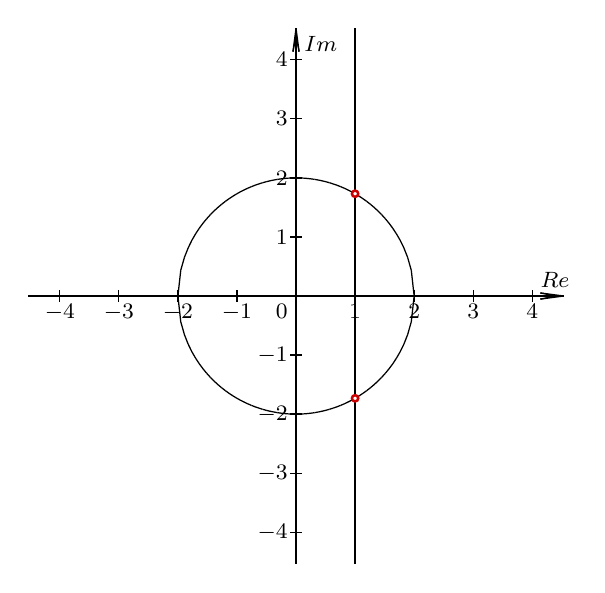
\begin{tikzpicture}
                    % \clip (0,0) rectangle (14.000000,10.000000);
                    {\footnotesize

                    % Changing color 215 183 183
                    \definecolor{r215g183b183}{rgb}{0.843137,0.717647,0.717647}%
                    \color{r215g183b183}% 

                    % Changing color 0 0 0
                    \definecolor{r0g0b0}{rgb}{0.000000,0.000000,0.000000}%
                    \color{r0g0b0}% 

                    % Drawing 2D Cartesian system
                    \draw (4.100000,4.000000) node [anchor=north east] { $0$ };%
                    \draw [line width=0.016cm] (4.100000,3.925000) -- (4.100000,4.075000);%
                    \draw (4.850000,4.000000) node [anchor=north] { $1$ };%
                    \draw [line width=0.016cm] (4.850000,3.925000) -- (4.850000,4.075000);%
                    \draw (5.600000,4.000000) node [anchor=north] { $2$ };%
                    \draw [line width=0.016cm] (5.600000,3.925000) -- (5.600000,4.075000);%
                    \draw (6.350000,4.000000) node [anchor=north] { $3$ };%
                    \draw [line width=0.016cm] (6.350000,3.925000) -- (6.350000,4.075000);%
                    \draw (7.100000,4.000000) node [anchor=north] { $4$ };%
                    \draw [line width=0.016cm] (7.100000,3.925000) -- (7.100000,4.075000);%
                    \draw (3.350000,4.000000) node [anchor=north] { $-1$ };%
                    \draw [line width=0.016cm] (3.350000,3.925000) -- (3.350000,4.075000);%
                    \draw (2.600000,4.000000) node [anchor=north] { $-2$ };%
                    \draw [line width=0.016cm] (2.600000,3.925000) -- (2.600000,4.075000);%
                    \draw (1.850000,4.000000) node [anchor=north] { $-3$ };%
                    \draw [line width=0.016cm] (1.850000,3.925000) -- (1.850000,4.075000);%
                    \draw (1.100000,4.000000) node [anchor=north] { $-4$ };%
                    \draw [line width=0.016cm] (1.100000,3.925000) -- (1.100000,4.075000);%
                    \draw (4.100000,4.750000) node [anchor=east] { $1$ };%
                    \draw [line width=0.016cm] (4.025000,4.750000) -- (4.175000,4.750000);%
                    \draw (4.100000,5.500000) node [anchor=east] { $2$ };%
                    \draw [line width=0.016cm] (4.025000,5.500000) -- (4.175000,5.500000);%
                    \draw (4.100000,6.250000) node [anchor=east] { $3$ };%
                    \draw [line width=0.016cm] (4.025000,6.250000) -- (4.175000,6.250000);%
                    \draw (4.100000,7.000000) node [anchor=east] { $4$ };%
                    \draw [line width=0.016cm] (4.025000,7.000000) -- (4.175000,7.000000);%
                    \draw (4.100000,3.250000) node [anchor=east] { $-1$ };%
                    \draw [line width=0.016cm] (4.025000,3.250000) -- (4.175000,3.250000);%
                    \draw (4.100000,2.500000) node [anchor=east] { $-2$ };%
                    \draw [line width=0.016cm] (4.025000,2.500000) -- (4.175000,2.500000);%
                    \draw (4.100000,1.750000) node [anchor=east] { $-3$ };%
                    \draw [line width=0.016cm] (4.025000,1.750000) -- (4.175000,1.750000);%
                    \draw (4.100000,1.000000) node [anchor=east] { $-4$ };%
                    \draw [line width=0.016cm] (4.025000,1.000000) -- (4.175000,1.000000);%
                    \draw [line width=0.016cm] (0.700000,4.000000) -- (7.500000,4.000000);%
                    \draw [line width=0.016cm] (7.202567,4.039158) -- (7.500000,4.000000);%
                    \draw [line width=0.016cm] (7.202567,4.039158) -- (7.400000,4.000000);%
                    \draw [line width=0.016cm] (7.202567,3.960842) -- (7.500000,4.000000);%
                    \draw [line width=0.016cm] (7.202567,3.960842) -- (7.400000,4.000000);%
                    \draw [line width=0.016cm] (4.100000,0.600000) -- (4.100000,7.400000);%
                    \draw [line width=0.016cm] (4.060842,7.102567) -- (4.100000,7.400000);%
                    \draw [line width=0.016cm] (4.060842,7.102567) -- (4.100000,7.300000);%
                    \draw [line width=0.016cm] (4.139158,7.102567) -- (4.100000,7.400000);%
                    \draw [line width=0.016cm] (4.139158,7.102567) -- (4.100000,7.300000);%

                    % Marking point Im
                    \draw (4.100000,7.000000) node [anchor=south west] { $Im$ };%

                    % Marking point Re
                    \draw (7.100000,4.000000) node [anchor=south west] { $Re$ };%

                    % Drawing 2D ang conic k
                    \draw [line width=0.016cm] (2.600000,4.000000) -- (2.618056,4.163577);%
                    \draw [line width=0.016cm] (2.618056,4.163577) -- (2.636111,4.327153);%
                    \draw [line width=0.016cm] (2.600000,4.000000) -- (2.618056,3.836423);%
                    \draw [line width=0.016cm] (2.618056,3.836423) -- (2.636111,3.672847);%
                    \draw [line width=0.016cm] (2.636111,4.327153) -- (2.683333,4.493007);%
                    \draw [line width=0.016cm] (2.636111,3.672847) -- (2.683333,3.506993);%
                    \draw [line width=0.016cm] (2.683333,4.493007) -- (2.730556,4.612064);%
                    \draw [line width=0.016cm] (2.683333,3.506993) -- (2.730556,3.387936);%
                    \draw [line width=0.016cm] (2.730556,4.612064) -- (2.777778,4.708328);%
                    \draw [line width=0.016cm] (2.730556,3.387936) -- (2.777778,3.291672);%
                    \draw [line width=0.016cm] (2.777778,4.708328) -- (2.825000,4.790174);%
                    \draw [line width=0.016cm] (2.777778,3.291672) -- (2.825000,3.209826);%
                    \draw [line width=0.016cm] (2.825000,4.790174) -- (2.872222,4.861720);%
                    \draw [line width=0.016cm] (2.825000,3.209826) -- (2.872222,3.138280);%
                    \draw [line width=0.016cm] (2.872222,4.861720) -- (2.919444,4.925359);%
                    \draw [line width=0.016cm] (2.872222,3.138280) -- (2.919444,3.074641);%
                    \draw [line width=0.016cm] (2.919444,4.925359) -- (2.966667,4.982627);%
                    \draw [line width=0.016cm] (2.919444,3.074641) -- (2.966667,3.017373);%
                    \draw [line width=0.016cm] (2.966667,4.982627) -- (3.013889,5.034583);%
                    \draw [line width=0.016cm] (2.966667,3.017373) -- (3.013889,2.965417);%
                    \draw [line width=0.016cm] (3.013889,5.034583) -- (3.061111,5.081993);%
                    \draw [line width=0.016cm] (3.013889,2.965417) -- (3.061111,2.918007);%
                    \draw [line width=0.016cm] (3.061111,5.081993) -- (3.108333,5.125432);%
                    \draw [line width=0.016cm] (3.061111,2.918007) -- (3.108333,2.874568);%
                    \draw [line width=0.016cm] (3.108333,5.125432) -- (3.155556,5.165343);%
                    \draw [line width=0.016cm] (3.108333,2.874568) -- (3.155556,2.834657);%
                    \draw [line width=0.016cm] (3.155556,5.165343) -- (3.202778,5.202078);%
                    \draw [line width=0.016cm] (3.155556,2.834657) -- (3.202778,2.797922);%
                    \draw [line width=0.016cm] (3.202778,5.202078) -- (3.250000,5.235921);%
                    \draw [line width=0.016cm] (3.202778,2.797922) -- (3.250000,2.764079);%
                    \draw [line width=0.016cm] (3.250000,5.235921) -- (3.297222,5.267102);%
                    \draw [line width=0.016cm] (3.250000,2.764079) -- (3.297222,2.732898);%
                    \draw [line width=0.016cm] (3.297222,5.267102) -- (3.344444,5.295815);%
                    \draw [line width=0.016cm] (3.297222,2.732898) -- (3.344444,2.704185);%
                    \draw [line width=0.016cm] (3.344444,5.295815) -- (3.391667,5.322219);%
                    \draw [line width=0.016cm] (3.344444,2.704185) -- (3.391667,2.677781);%
                    \draw [line width=0.016cm] (3.391667,5.322219) -- (3.438889,5.346452);%
                    \draw [line width=0.016cm] (3.391667,2.677781) -- (3.438889,2.653548);%
                    \draw [line width=0.016cm] (3.438889,5.346452) -- (3.486111,5.368627);%
                    \draw [line width=0.016cm] (3.438889,2.653548) -- (3.486111,2.631373);%
                    \draw [line width=0.016cm] (3.486111,5.368627) -- (3.533333,5.388844);%
                    \draw [line width=0.016cm] (3.486111,2.631373) -- (3.533333,2.611156);%
                    \draw [line width=0.016cm] (3.533333,5.388844) -- (3.580556,5.407188);%
                    \draw [line width=0.016cm] (3.533333,2.611156) -- (3.580556,2.592812);%
                    \draw [line width=0.016cm] (3.580556,5.407188) -- (3.627778,5.423730);%
                    \draw [line width=0.016cm] (3.580556,2.592812) -- (3.627778,2.576270);%
                    \draw [line width=0.016cm] (3.627778,5.423730) -- (3.675000,5.438532);%
                    \draw [line width=0.016cm] (3.627778,2.576270) -- (3.675000,2.561468);%
                    \draw [line width=0.016cm] (3.675000,5.438532) -- (3.722222,5.451649);%
                    \draw [line width=0.016cm] (3.675000,2.561468) -- (3.722222,2.548351);%
                    \draw [line width=0.016cm] (3.722222,5.451649) -- (3.769444,5.463124);%
                    \draw [line width=0.016cm] (3.722222,2.548351) -- (3.769444,2.536876);%
                    \draw [line width=0.016cm] (3.769444,5.463124) -- (3.816667,5.472998);%
                    \draw [line width=0.016cm] (3.769444,2.536876) -- (3.816667,2.527002);%
                    \draw [line width=0.016cm] (3.816667,5.472998) -- (3.863889,5.481301);%
                    \draw [line width=0.016cm] (3.816667,2.527002) -- (3.863889,2.518699);%
                    \draw [line width=0.016cm] (3.863889,5.481301) -- (3.911111,5.488059);%
                    \draw [line width=0.016cm] (3.863889,2.518699) -- (3.911111,2.511941);%
                    \draw [line width=0.016cm] (3.911111,5.488059) -- (3.958333,5.493295);%
                    \draw [line width=0.016cm] (3.911111,2.511941) -- (3.958333,2.506705);%
                    \draw [line width=0.016cm] (3.958333,5.493295) -- (4.005556,5.497024);%
                    \draw [line width=0.016cm] (3.958333,2.506705) -- (4.005556,2.502976);%
                    \draw [line width=0.016cm] (4.005556,5.497024) -- (4.052778,5.499257);%
                    \draw [line width=0.016cm] (4.005556,2.502976) -- (4.052778,2.500743);%
                    \draw [line width=0.016cm] (4.052778,5.499257) -- (4.100000,5.500000);%
                    \draw [line width=0.016cm] (4.052778,2.500743) -- (4.100000,2.500000);%
                    \draw [line width=0.016cm] (4.100000,5.500000) -- (4.147222,5.499257);%
                    \draw [line width=0.016cm] (4.100000,2.500000) -- (4.147222,2.500743);%
                    \draw [line width=0.016cm] (4.147222,5.499257) -- (4.194444,5.497024);%
                    \draw [line width=0.016cm] (4.147222,2.500743) -- (4.194444,2.502976);%
                    \draw [line width=0.016cm] (4.194444,5.497024) -- (4.241667,5.493295);%
                    \draw [line width=0.016cm] (4.194444,2.502976) -- (4.241667,2.506705);%
                    \draw [line width=0.016cm] (4.241667,5.493295) -- (4.288889,5.488059);%
                    \draw [line width=0.016cm] (4.241667,2.506705) -- (4.288889,2.511941);%
                    \draw [line width=0.016cm] (4.288889,5.488059) -- (4.336111,5.481301);%
                    \draw [line width=0.016cm] (4.288889,2.511941) -- (4.336111,2.518699);%
                    \draw [line width=0.016cm] (4.336111,5.481301) -- (4.383333,5.472998);%
                    \draw [line width=0.016cm] (4.336111,2.518699) -- (4.383333,2.527002);%
                    \draw [line width=0.016cm] (4.383333,5.472998) -- (4.430556,5.463124);%
                    \draw [line width=0.016cm] (4.383333,2.527002) -- (4.430556,2.536876);%
                    \draw [line width=0.016cm] (4.430556,5.463124) -- (4.477778,5.451649);%
                    \draw [line width=0.016cm] (4.430556,2.536876) -- (4.477778,2.548351);%
                    \draw [line width=0.016cm] (4.477778,5.451649) -- (4.525000,5.438532);%
                    \draw [line width=0.016cm] (4.477778,2.548351) -- (4.525000,2.561468);%
                    \draw [line width=0.016cm] (4.525000,5.438532) -- (4.572222,5.423730);%
                    \draw [line width=0.016cm] (4.525000,2.561468) -- (4.572222,2.576270);%
                    \draw [line width=0.016cm] (4.572222,5.423730) -- (4.619444,5.407188);%
                    \draw [line width=0.016cm] (4.572222,2.576270) -- (4.619444,2.592812);%
                    \draw [line width=0.016cm] (4.619444,5.407188) -- (4.666667,5.388844);%
                    \draw [line width=0.016cm] (4.619444,2.592812) -- (4.666667,2.611156);%
                    \draw [line width=0.016cm] (4.666667,5.388844) -- (4.713889,5.368627);%
                    \draw [line width=0.016cm] (4.666667,2.611156) -- (4.713889,2.631373);%
                    \draw [line width=0.016cm] (4.713889,5.368627) -- (4.761111,5.346452);%
                    \draw [line width=0.016cm] (4.713889,2.631373) -- (4.761111,2.653548);%
                    \draw [line width=0.016cm] (4.761111,5.346452) -- (4.808333,5.322219);%
                    \draw [line width=0.016cm] (4.761111,2.653548) -- (4.808333,2.677781);%
                    \draw [line width=0.016cm] (4.808333,5.322219) -- (4.815037,5.318471);%
                    \draw [line width=0.016cm] (4.808333,2.677781) -- (4.815037,2.681529);%
                    \draw [line width=0.016cm] (4.884246,5.278370) -- (4.902778,5.267102);%
                    \draw [line width=0.016cm] (4.884246,2.721630) -- (4.902778,2.732898);%
                    \draw [line width=0.016cm] (4.902778,5.267102) -- (4.950000,5.235921);%
                    \draw [line width=0.016cm] (4.902778,2.732898) -- (4.950000,2.764079);%
                    \draw [line width=0.016cm] (4.950000,5.235921) -- (4.997222,5.202078);%
                    \draw [line width=0.016cm] (4.950000,2.764079) -- (4.997222,2.797922);%
                    \draw [line width=0.016cm] (4.997222,5.202078) -- (5.044444,5.165343);%
                    \draw [line width=0.016cm] (4.997222,2.797922) -- (5.044444,2.834657);%
                    \draw [line width=0.016cm] (5.044444,5.165343) -- (5.091667,5.125432);%
                    \draw [line width=0.016cm] (5.044444,2.834657) -- (5.091667,2.874568);%
                    \draw [line width=0.016cm] (5.091667,5.125432) -- (5.138889,5.081993);%
                    \draw [line width=0.016cm] (5.091667,2.874568) -- (5.138889,2.918007);%
                    \draw [line width=0.016cm] (5.138889,5.081993) -- (5.186111,5.034583);%
                    \draw [line width=0.016cm] (5.138889,2.918007) -- (5.186111,2.965417);%
                    \draw [line width=0.016cm] (5.186111,5.034583) -- (5.233333,4.982627);%
                    \draw [line width=0.016cm] (5.186111,2.965417) -- (5.233333,3.017373);%
                    \draw [line width=0.016cm] (5.233333,4.982627) -- (5.280556,4.925359);%
                    \draw [line width=0.016cm] (5.233333,3.017373) -- (5.280556,3.074641);%
                    \draw [line width=0.016cm] (5.280556,4.925359) -- (5.327778,4.861720);%
                    \draw [line width=0.016cm] (5.280556,3.074641) -- (5.327778,3.138280);%
                    \draw [line width=0.016cm] (5.327778,4.861720) -- (5.375000,4.790174);%
                    \draw [line width=0.016cm] (5.327778,3.138280) -- (5.375000,3.209826);%
                    \draw [line width=0.016cm] (5.375000,4.790174) -- (5.422222,4.708328);%
                    \draw [line width=0.016cm] (5.375000,3.209826) -- (5.422222,3.291672);%
                    \draw [line width=0.016cm] (5.422222,4.708328) -- (5.469444,4.612064);%
                    \draw [line width=0.016cm] (5.422222,3.291672) -- (5.469444,3.387936);%
                    \draw [line width=0.016cm] (5.469444,4.612064) -- (5.516667,4.493007);%
                    \draw [line width=0.016cm] (5.469444,3.387936) -- (5.516667,3.506993);%
                    \draw [line width=0.016cm] (5.516667,4.493007) -- (5.563889,4.327153);%
                    \draw [line width=0.016cm] (5.516667,3.506993) -- (5.563889,3.672847);%
                    \draw [line width=0.016cm] (5.600000,4.000000) -- (5.581944,4.163577);%
                    \draw [line width=0.016cm] (5.581944,4.163577) -- (5.563889,4.327153);%
                    \draw [line width=0.016cm] (5.600000,4.000000) -- (5.581944,3.836423);%
                    \draw [line width=0.016cm] (5.581944,3.836423) -- (5.563889,3.672847);%

                    % Drawing 2D ang line l
                    \draw [line width=0.016cm] (4.850000,0.600000) -- (4.850000,2.660962);%
                    \draw [line width=0.016cm] (4.850000,2.740962) -- (4.850000,5.259038);%
                    \draw [line width=0.016cm] (4.850000,5.339038) -- (4.850000,7.400000);%

                    % Changing color 204 0 0
                    \definecolor{r204g0b0}{rgb}{0.800000,0.000000,0.000000}%
                    \color{r204g0b0}% 

                    % Marking point X1 by circle
                    \draw [line width=0.032cm] (4.850000,5.299038) circle (0.040000);%

                    % Marking point X2 by circle
                    \draw [line width=0.032cm] (4.850000,2.700962) circle (0.040000);%
                    \color{black}
                    }
                    \end{tikzpicture}

                \end{figure}
                
            \end{exampleblock}}


        \end{frame}


        \begin{frame}

            \only<2->{\begin{exampleblock}{Naloga}
                Za označeno množico točk zapišite, katermu pogoju ustreza.
                \vskip-1em
                \begin{figure}[H]
                    \centering
                    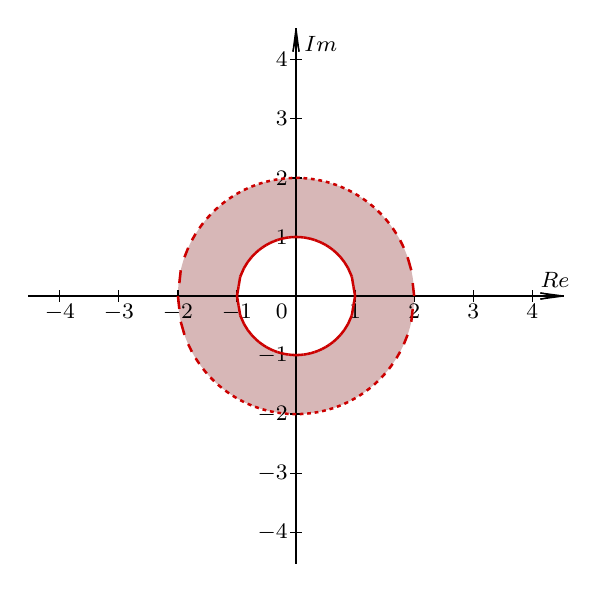
\begin{tikzpicture}
                    % \clip (0,0) rectangle (14.000000,10.000000);
                    {\footnotesize

                    % Changing color 215 183 183
                    \definecolor{r215g183b183}{rgb}{0.843137,0.717647,0.717647}%
                    \color{r215g183b183}% 

                    % Filling circle S B
                    \fill (4.100000,4.000000) circle (1.500000);%

                    % Changing color 255 255 255
                    \definecolor{r255g255b255}{rgb}{1.000000,1.000000,1.000000}%
                    \color{r255g255b255}% 

                    % Filling circle S A
                    \fill (4.100000,4.000000) circle (0.750000);%

                    % Changing color 0 0 0
                    \definecolor{r0g0b0}{rgb}{0.000000,0.000000,0.000000}%
                    \color{r0g0b0}% 

                    % Drawing 2D Cartesian system
                    \draw (4.100000,4.000000) node [anchor=north east] { $0$ };%
                    \draw [line width=0.016cm] (4.100000,3.925000) -- (4.100000,4.075000);%
                    \draw (4.850000,4.000000) node [anchor=north] { $1$ };%
                    \draw [line width=0.016cm] (4.850000,3.925000) -- (4.850000,4.075000);%
                    \draw (5.600000,4.000000) node [anchor=north] { $2$ };%
                    \draw [line width=0.016cm] (5.600000,3.925000) -- (5.600000,4.075000);%
                    \draw (6.350000,4.000000) node [anchor=north] { $3$ };%
                    \draw [line width=0.016cm] (6.350000,3.925000) -- (6.350000,4.075000);%
                    \draw (7.100000,4.000000) node [anchor=north] { $4$ };%
                    \draw [line width=0.016cm] (7.100000,3.925000) -- (7.100000,4.075000);%
                    \draw (3.350000,4.000000) node [anchor=north] { $-1$ };%
                    \draw [line width=0.016cm] (3.350000,3.925000) -- (3.350000,4.075000);%
                    \draw (2.600000,4.000000) node [anchor=north] { $-2$ };%
                    \draw [line width=0.016cm] (2.600000,3.925000) -- (2.600000,4.075000);%
                    \draw (1.850000,4.000000) node [anchor=north] { $-3$ };%
                    \draw [line width=0.016cm] (1.850000,3.925000) -- (1.850000,4.075000);%
                    \draw (1.100000,4.000000) node [anchor=north] { $-4$ };%
                    \draw [line width=0.016cm] (1.100000,3.925000) -- (1.100000,4.075000);%
                    \draw (4.100000,4.750000) node [anchor=east] { $1$ };%
                    \draw [line width=0.016cm] (4.025000,4.750000) -- (4.175000,4.750000);%
                    \draw (4.100000,5.500000) node [anchor=east] { $2$ };%
                    \draw [line width=0.016cm] (4.025000,5.500000) -- (4.175000,5.500000);%
                    \draw (4.100000,6.250000) node [anchor=east] { $3$ };%
                    \draw [line width=0.016cm] (4.025000,6.250000) -- (4.175000,6.250000);%
                    \draw (4.100000,7.000000) node [anchor=east] { $4$ };%
                    \draw [line width=0.016cm] (4.025000,7.000000) -- (4.175000,7.000000);%
                    \draw (4.100000,3.250000) node [anchor=east] { $-1$ };%
                    \draw [line width=0.016cm] (4.025000,3.250000) -- (4.175000,3.250000);%
                    \draw (4.100000,2.500000) node [anchor=east] { $-2$ };%
                    \draw [line width=0.016cm] (4.025000,2.500000) -- (4.175000,2.500000);%
                    \draw (4.100000,1.750000) node [anchor=east] { $-3$ };%
                    \draw [line width=0.016cm] (4.025000,1.750000) -- (4.175000,1.750000);%
                    \draw (4.100000,1.000000) node [anchor=east] { $-4$ };%
                    \draw [line width=0.016cm] (4.025000,1.000000) -- (4.175000,1.000000);%
                    \draw [line width=0.016cm] (0.700000,4.000000) -- (7.500000,4.000000);%
                    \draw [line width=0.016cm] (7.202567,4.039158) -- (7.500000,4.000000);%
                    \draw [line width=0.016cm] (7.202567,4.039158) -- (7.400000,4.000000);%
                    \draw [line width=0.016cm] (7.202567,3.960842) -- (7.500000,4.000000);%
                    \draw [line width=0.016cm] (7.202567,3.960842) -- (7.400000,4.000000);%
                    \draw [line width=0.016cm] (4.100000,0.600000) -- (4.100000,7.400000);%
                    \draw [line width=0.016cm] (4.060842,7.102567) -- (4.100000,7.400000);%
                    \draw [line width=0.016cm] (4.060842,7.102567) -- (4.100000,7.300000);%
                    \draw [line width=0.016cm] (4.139158,7.102567) -- (4.100000,7.400000);%
                    \draw [line width=0.016cm] (4.139158,7.102567) -- (4.100000,7.300000);%

                    % Marking point Im
                    \draw (4.100000,7.000000) node [anchor=south west] { $Im$ };%

                    % Marking point Re
                    \draw (7.100000,4.000000) node [anchor=south west] { $Re$ };%

                    % Changing color 204 0 0
                    \definecolor{r204g0b0}{rgb}{0.800000,0.000000,0.000000}%
                    \color{r204g0b0}% 

                    % Drawing 2D ang conic k
                    \draw [line width=0.032cm] (3.350000,4.000000) -- (3.370833,4.123252);%
                    \draw [line width=0.032cm] (3.370833,4.123252) -- (3.391667,4.246503);%
                    \draw [line width=0.032cm] (3.350000,4.000000) -- (3.370833,3.876748);%
                    \draw [line width=0.032cm] (3.370833,3.876748) -- (3.391667,3.753497);%
                    \draw [line width=0.032cm] (3.391667,4.246503) -- (3.438889,4.354164);%
                    \draw [line width=0.032cm] (3.391667,3.753497) -- (3.438889,3.645836);%
                    \draw [line width=0.032cm] (3.438889,4.354164) -- (3.486111,4.430860);%
                    \draw [line width=0.032cm] (3.438889,3.645836) -- (3.486111,3.569140);%
                    \draw [line width=0.032cm] (3.486111,4.430860) -- (3.533333,4.491313);%
                    \draw [line width=0.032cm] (3.486111,3.569140) -- (3.533333,3.508687);%
                    \draw [line width=0.032cm] (3.533333,4.491313) -- (3.580556,4.540997);%
                    \draw [line width=0.032cm] (3.533333,3.508687) -- (3.580556,3.459003);%
                    \draw [line width=0.032cm] (3.580556,4.540997) -- (3.627778,4.582672);%
                    \draw [line width=0.032cm] (3.580556,3.459003) -- (3.627778,3.417328);%
                    \draw [line width=0.032cm] (3.627778,4.582672) -- (3.675000,4.617960);%
                    \draw [line width=0.032cm] (3.627778,3.417328) -- (3.675000,3.382040);%
                    \draw [line width=0.032cm] (3.675000,4.617960) -- (3.722222,4.647907);%
                    \draw [line width=0.032cm] (3.675000,3.382040) -- (3.722222,3.352093);%
                    \draw [line width=0.032cm] (3.722222,4.647907) -- (3.769444,4.673226);%
                    \draw [line width=0.032cm] (3.722222,3.352093) -- (3.769444,3.326774);%
                    \draw [line width=0.032cm] (3.769444,4.673226) -- (3.816667,4.694422);%
                    \draw [line width=0.032cm] (3.769444,3.326774) -- (3.816667,3.305578);%
                    \draw [line width=0.032cm] (3.816667,4.694422) -- (3.863889,4.711865);%
                    \draw [line width=0.032cm] (3.816667,3.305578) -- (3.863889,3.288135);%
                    \draw [line width=0.032cm] (3.863889,4.711865) -- (3.911111,4.725824);%
                    \draw [line width=0.032cm] (3.863889,3.288135) -- (3.911111,3.274176);%
                    \draw [line width=0.032cm] (3.911111,4.725824) -- (3.958333,4.736499);%
                    \draw [line width=0.032cm] (3.911111,3.274176) -- (3.958333,3.263501);%
                    \draw [line width=0.032cm] (3.958333,4.736499) -- (4.005556,4.744030);%
                    \draw [line width=0.032cm] (3.958333,3.263501) -- (4.005556,3.255970);%
                    \draw [line width=0.032cm] (4.005556,4.744030) -- (4.052778,4.748512);%
                    \draw [line width=0.032cm] (4.005556,3.255970) -- (4.052778,3.251488);%
                    \draw [line width=0.032cm] (4.052778,4.748512) -- (4.100000,4.750000);%
                    \draw [line width=0.032cm] (4.052778,3.251488) -- (4.100000,3.250000);%
                    \draw [line width=0.032cm] (4.100000,4.750000) -- (4.147222,4.748512);%
                    \draw [line width=0.032cm] (4.100000,3.250000) -- (4.147222,3.251488);%
                    \draw [line width=0.032cm] (4.147222,4.748512) -- (4.194444,4.744030);%
                    \draw [line width=0.032cm] (4.147222,3.251488) -- (4.194444,3.255970);%
                    \draw [line width=0.032cm] (4.194444,4.744030) -- (4.241667,4.736499);%
                    \draw [line width=0.032cm] (4.194444,3.255970) -- (4.241667,3.263501);%
                    \draw [line width=0.032cm] (4.241667,4.736499) -- (4.288889,4.725824);%
                    \draw [line width=0.032cm] (4.241667,3.263501) -- (4.288889,3.274176);%
                    \draw [line width=0.032cm] (4.288889,4.725824) -- (4.336111,4.711865);%
                    \draw [line width=0.032cm] (4.288889,3.274176) -- (4.336111,3.288135);%
                    \draw [line width=0.032cm] (4.336111,4.711865) -- (4.383333,4.694422);%
                    \draw [line width=0.032cm] (4.336111,3.288135) -- (4.383333,3.305578);%
                    \draw [line width=0.032cm] (4.383333,4.694422) -- (4.430556,4.673226);%
                    \draw [line width=0.032cm] (4.383333,3.305578) -- (4.430556,3.326774);%
                    \draw [line width=0.032cm] (4.430556,4.673226) -- (4.477778,4.647907);%
                    \draw [line width=0.032cm] (4.430556,3.326774) -- (4.477778,3.352093);%
                    \draw [line width=0.032cm] (4.477778,4.647907) -- (4.525000,4.617960);%
                    \draw [line width=0.032cm] (4.477778,3.352093) -- (4.525000,3.382040);%
                    \draw [line width=0.032cm] (4.525000,4.617960) -- (4.572222,4.582672);%
                    \draw [line width=0.032cm] (4.525000,3.382040) -- (4.572222,3.417328);%
                    \draw [line width=0.032cm] (4.572222,4.582672) -- (4.619444,4.540997);%
                    \draw [line width=0.032cm] (4.572222,3.417328) -- (4.619444,3.459003);%
                    \draw [line width=0.032cm] (4.619444,4.540997) -- (4.666667,4.491313);%
                    \draw [line width=0.032cm] (4.619444,3.459003) -- (4.666667,3.508687);%
                    \draw [line width=0.032cm] (4.666667,4.491313) -- (4.713889,4.430860);%
                    \draw [line width=0.032cm] (4.666667,3.508687) -- (4.713889,3.569140);%
                    \draw [line width=0.032cm] (4.713889,4.430860) -- (4.761111,4.354164);%
                    \draw [line width=0.032cm] (4.713889,3.569140) -- (4.761111,3.645836);%
                    \draw [line width=0.032cm] (4.761111,4.354164) -- (4.808333,4.246503);%
                    \draw [line width=0.032cm] (4.761111,3.645836) -- (4.808333,3.753497);%
                    \draw [line width=0.032cm] (4.850000,4.000000) -- (4.829167,4.123252);%
                    \draw [line width=0.032cm] (4.829167,4.123252) -- (4.808333,4.246503);%
                    \draw [line width=0.032cm] (4.850000,4.000000) -- (4.829167,3.876748);%
                    \draw [line width=0.032cm] (4.829167,3.876748) -- (4.808333,3.753497);%

                    % Drawing 2D ang conic k2
                    \draw [line width=0.032cm] (2.618056,4.163577) -- (2.636111,4.327153);%
                    \draw [line width=0.032cm] (2.600000,4.000000) -- (2.618056,3.836423);%
                    \draw [line width=0.032cm] (2.636111,3.672847) -- (2.683333,3.506993);%
                    \draw [line width=0.032cm] (2.683333,4.493007) -- (2.730556,4.612064);%
                    \draw [line width=0.032cm] (2.730556,3.387936) -- (2.777778,3.291672);%
                    \draw [line width=0.032cm] (2.777778,4.708328) -- (2.825000,4.790174);%
                    \draw [line width=0.032cm] (2.825000,3.209826) -- (2.872222,3.138280);%
                    \draw [line width=0.032cm] (2.872222,4.861720) -- (2.919444,4.925359);%
                    \draw [line width=0.032cm] (2.919444,3.074641) -- (2.966667,3.017373);%
                    \draw [line width=0.032cm] (2.966667,4.982627) -- (3.013889,5.034583);%
                    \draw [line width=0.032cm] (3.013889,2.965417) -- (3.061111,2.918007);%
                    \draw [line width=0.032cm] (3.061111,5.081993) -- (3.108333,5.125432);%
                    \draw [line width=0.032cm] (3.108333,2.874568) -- (3.155556,2.834657);%
                    \draw [line width=0.032cm] (3.155556,5.165343) -- (3.202778,5.202078);%
                    \draw [line width=0.032cm] (3.202778,2.797922) -- (3.250000,2.764079);%
                    \draw [line width=0.032cm] (3.250000,5.235921) -- (3.297222,5.267102);%
                    \draw [line width=0.032cm] (3.297222,2.732898) -- (3.344444,2.704185);%
                    \draw [line width=0.032cm] (3.344444,5.295815) -- (3.391667,5.322219);%
                    \draw [line width=0.032cm] (3.391667,2.677781) -- (3.438889,2.653548);%
                    \draw [line width=0.032cm] (3.438889,5.346452) -- (3.486111,5.368627);%
                    \draw [line width=0.032cm] (3.486111,2.631373) -- (3.533333,2.611156);%
                    \draw [line width=0.032cm] (3.533333,5.388844) -- (3.580556,5.407188);%
                    \draw [line width=0.032cm] (3.580556,2.592812) -- (3.627778,2.576270);%
                    \draw [line width=0.032cm] (3.627778,5.423730) -- (3.675000,5.438532);%
                    \draw [line width=0.032cm] (3.675000,2.561468) -- (3.722222,2.548351);%
                    \draw [line width=0.032cm] (3.722222,5.451649) -- (3.769444,5.463124);%
                    \draw [line width=0.032cm] (3.769444,2.536876) -- (3.816667,2.527002);%
                    \draw [line width=0.032cm] (3.816667,5.472998) -- (3.863889,5.481301);%
                    \draw [line width=0.032cm] (3.863889,2.518699) -- (3.911111,2.511941);%
                    \draw [line width=0.032cm] (3.911111,5.488059) -- (3.958333,5.493295);%
                    \draw [line width=0.032cm] (3.958333,2.506705) -- (4.005556,2.502976);%
                    \draw [line width=0.032cm] (4.005556,5.497024) -- (4.052778,5.499257);%
                    \draw [line width=0.032cm] (4.052778,2.500743) -- (4.100000,2.500000);%
                    \draw [line width=0.032cm] (4.100000,5.500000) -- (4.147222,5.499257);%
                    \draw [line width=0.032cm] (4.147222,2.500743) -- (4.194444,2.502976);%
                    \draw [line width=0.032cm] (4.194444,5.497024) -- (4.241667,5.493295);%
                    \draw [line width=0.032cm] (4.241667,2.506705) -- (4.288889,2.511941);%
                    \draw [line width=0.032cm] (4.288889,5.488059) -- (4.336111,5.481301);%
                    \draw [line width=0.032cm] (4.336111,2.518699) -- (4.383333,2.527002);%
                    \draw [line width=0.032cm] (4.383333,5.472998) -- (4.430556,5.463124);%
                    \draw [line width=0.032cm] (4.430556,2.536876) -- (4.477778,2.548351);%
                    \draw [line width=0.032cm] (4.477778,5.451649) -- (4.525000,5.438532);%
                    \draw [line width=0.032cm] (4.525000,2.561468) -- (4.572222,2.576270);%
                    \draw [line width=0.032cm] (4.572222,5.423730) -- (4.619444,5.407188);%
                    \draw [line width=0.032cm] (4.619444,2.592812) -- (4.666667,2.611156);%
                    \draw [line width=0.032cm] (4.666667,5.388844) -- (4.713889,5.368627);%
                    \draw [line width=0.032cm] (4.713889,2.631373) -- (4.761111,2.653548);%
                    \draw [line width=0.032cm] (4.761111,5.346452) -- (4.808333,5.322219);%
                    \draw [line width=0.032cm] (4.808333,2.677781) -- (4.855556,2.704185);%
                    \draw [line width=0.032cm] (4.855556,5.295815) -- (4.902778,5.267102);%
                    \draw [line width=0.032cm] (4.902778,2.732898) -- (4.950000,2.764079);%
                    \draw [line width=0.032cm] (4.950000,5.235921) -- (4.997222,5.202078);%
                    \draw [line width=0.032cm] (4.997222,2.797922) -- (5.044444,2.834657);%
                    \draw [line width=0.032cm] (5.044444,5.165343) -- (5.091667,5.125432);%
                    \draw [line width=0.032cm] (5.091667,2.874568) -- (5.138889,2.918007);%
                    \draw [line width=0.032cm] (5.138889,5.081993) -- (5.186111,5.034583);%
                    \draw [line width=0.032cm] (5.186111,2.965417) -- (5.233333,3.017373);%
                    \draw [line width=0.032cm] (5.233333,4.982627) -- (5.280556,4.925359);%
                    \draw [line width=0.032cm] (5.280556,3.074641) -- (5.327778,3.138280);%
                    \draw [line width=0.032cm] (5.327778,4.861720) -- (5.375000,4.790174);%
                    \draw [line width=0.032cm] (5.375000,3.209826) -- (5.422222,3.291672);%
                    \draw [line width=0.032cm] (5.422222,4.708328) -- (5.469444,4.612064);%
                    \draw [line width=0.032cm] (5.469444,3.387936) -- (5.516667,3.506993);%
                    \draw [line width=0.032cm] (5.516667,4.493007) -- (5.563889,4.327153);%
                    \draw [line width=0.032cm] (5.600000,4.000000) -- (5.581944,4.163577);%
                    \draw [line width=0.032cm] (5.581944,3.836423) -- (5.563889,3.672847);%
                    \color{black}
                    }
                    \end{tikzpicture}
                    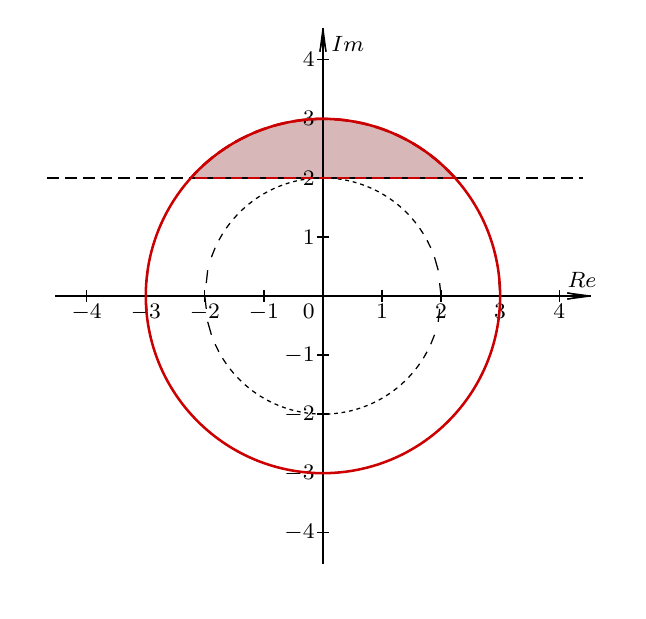
\begin{tikzpicture}
                    % \clip (0,0) rectangle (14.000000,10.000000);
                    {\footnotesize

                    % Changing color 183 183 183
                    \definecolor{r183g183b183}{rgb}{0.717647,0.717647,0.717647}%
                    \color{r183g183b183}% 

                    % Filling circle S A
                    \fill (4.100000,4.000000) circle (2.250000);%

                    % Changing color 215 183 183
                    \definecolor{r215g183b183}{rgb}{0.843137,0.717647,0.717647}%
                    \color{r215g183b183}% 

                    % Filling circle arc S X1 96.00
                    \fill (4.100000,4.000000) -- (5.777051,5.500000) -- (5.772076,5.505544) arc (42:137:2.250000 and 2.250000) -- (2.432918,5.511071) -- cycle;%

                    % Changing color 255 255 255
                    \definecolor{r255g255b255}{rgb}{1.000000,1.000000,1.000000}%
                    \color{r255g255b255}% 

                    % Filling circle S B
                    \fill (4.100000,4.000000) circle (1.500000);%

                    % Filling rectangle left-bottom: E right-top: G
                    \fill (0.350000,5.500000) -- (7.850000,5.500000) -- (7.850000,0.250000) -- (0.350000,0.250000);%

                    % Changing color 0 0 0
                    \definecolor{r0g0b0}{rgb}{0.000000,0.000000,0.000000}%
                    \color{r0g0b0}% 

                    % Drawing 2D Cartesian system
                    \draw (4.100000,4.000000) node [anchor=north east] { $0$ };%
                    \draw [line width=0.016cm] (4.100000,3.925000) -- (4.100000,4.075000);%
                    \draw (4.850000,4.000000) node [anchor=north] { $1$ };%
                    \draw [line width=0.016cm] (4.850000,3.925000) -- (4.850000,4.075000);%
                    \draw (5.600000,4.000000) node [anchor=north] { $2$ };%
                    \draw [line width=0.016cm] (5.600000,3.925000) -- (5.600000,4.075000);%
                    \draw (6.350000,4.000000) node [anchor=north] { $3$ };%
                    \draw [line width=0.016cm] (6.350000,3.925000) -- (6.350000,4.075000);%
                    \draw (7.100000,4.000000) node [anchor=north] { $4$ };%
                    \draw [line width=0.016cm] (7.100000,3.925000) -- (7.100000,4.075000);%
                    \draw (3.350000,4.000000) node [anchor=north] { $-1$ };%
                    \draw [line width=0.016cm] (3.350000,3.925000) -- (3.350000,4.075000);%
                    \draw (2.600000,4.000000) node [anchor=north] { $-2$ };%
                    \draw [line width=0.016cm] (2.600000,3.925000) -- (2.600000,4.075000);%
                    \draw (1.850000,4.000000) node [anchor=north] { $-3$ };%
                    \draw [line width=0.016cm] (1.850000,3.925000) -- (1.850000,4.075000);%
                    \draw (1.100000,4.000000) node [anchor=north] { $-4$ };%
                    \draw [line width=0.016cm] (1.100000,3.925000) -- (1.100000,4.075000);%
                    \draw (4.100000,4.750000) node [anchor=east] { $1$ };%
                    \draw [line width=0.016cm] (4.025000,4.750000) -- (4.175000,4.750000);%
                    \draw (4.100000,5.500000) node [anchor=east] { $2$ };%
                    \draw [line width=0.016cm] (4.025000,5.500000) -- (4.175000,5.500000);%
                    \draw (4.100000,6.250000) node [anchor=east] { $3$ };%
                    \draw [line width=0.016cm] (4.025000,6.250000) -- (4.175000,6.250000);%
                    \draw (4.100000,7.000000) node [anchor=east] { $4$ };%
                    \draw [line width=0.016cm] (4.025000,7.000000) -- (4.175000,7.000000);%
                    \draw (4.100000,3.250000) node [anchor=east] { $-1$ };%
                    \draw [line width=0.016cm] (4.025000,3.250000) -- (4.175000,3.250000);%
                    \draw (4.100000,2.500000) node [anchor=east] { $-2$ };%
                    \draw [line width=0.016cm] (4.025000,2.500000) -- (4.175000,2.500000);%
                    \draw (4.100000,1.750000) node [anchor=east] { $-3$ };%
                    \draw [line width=0.016cm] (4.025000,1.750000) -- (4.175000,1.750000);%
                    \draw (4.100000,1.000000) node [anchor=east] { $-4$ };%
                    \draw [line width=0.016cm] (4.025000,1.000000) -- (4.175000,1.000000);%
                    \draw [line width=0.016cm] (0.700000,4.000000) -- (7.500000,4.000000);%
                    \draw [line width=0.016cm] (7.202567,4.039158) -- (7.500000,4.000000);%
                    \draw [line width=0.016cm] (7.202567,4.039158) -- (7.400000,4.000000);%
                    \draw [line width=0.016cm] (7.202567,3.960842) -- (7.500000,4.000000);%
                    \draw [line width=0.016cm] (7.202567,3.960842) -- (7.400000,4.000000);%
                    \draw [line width=0.016cm] (4.100000,0.600000) -- (4.100000,7.400000);%
                    \draw [line width=0.016cm] (4.060842,7.102567) -- (4.100000,7.400000);%
                    \draw [line width=0.016cm] (4.060842,7.102567) -- (4.100000,7.300000);%
                    \draw [line width=0.016cm] (4.139158,7.102567) -- (4.100000,7.400000);%
                    \draw [line width=0.016cm] (4.139158,7.102567) -- (4.100000,7.300000);%

                    % Marking point Im
                    \draw (4.100000,7.000000) node [anchor=south west] { $Im$ };%

                    % Marking point Re
                    \draw (7.100000,4.000000) node [anchor=south west] { $Re$ };%

                    % Drawing 2D ang conic k
                    \draw [line width=0.016cm] (2.618056,4.163577) -- (2.636111,4.327153);%
                    \draw [line width=0.016cm] (2.600000,4.000000) -- (2.618056,3.836423);%
                    \draw [line width=0.016cm] (2.636111,3.672847) -- (2.683333,3.506993);%
                    \draw [line width=0.016cm] (2.683333,4.493007) -- (2.730556,4.612064);%
                    \draw [line width=0.016cm] (2.730556,3.387936) -- (2.777778,3.291672);%
                    \draw [line width=0.016cm] (2.777778,4.708328) -- (2.825000,4.790174);%
                    \draw [line width=0.016cm] (2.825000,3.209826) -- (2.872222,3.138280);%
                    \draw [line width=0.016cm] (2.872222,4.861720) -- (2.919444,4.925359);%
                    \draw [line width=0.016cm] (2.919444,3.074641) -- (2.966667,3.017373);%
                    \draw [line width=0.016cm] (2.966667,4.982627) -- (3.013889,5.034583);%
                    \draw [line width=0.016cm] (3.013889,2.965417) -- (3.061111,2.918007);%
                    \draw [line width=0.016cm] (3.061111,5.081993) -- (3.108333,5.125432);%
                    \draw [line width=0.016cm] (3.108333,2.874568) -- (3.155556,2.834657);%
                    \draw [line width=0.016cm] (3.155556,5.165343) -- (3.202778,5.202078);%
                    \draw [line width=0.016cm] (3.202778,2.797922) -- (3.250000,2.764079);%
                    \draw [line width=0.016cm] (3.250000,5.235921) -- (3.297222,5.267102);%
                    \draw [line width=0.016cm] (3.297222,2.732898) -- (3.344444,2.704185);%
                    \draw [line width=0.016cm] (3.344444,5.295815) -- (3.391667,5.322219);%
                    \draw [line width=0.016cm] (3.391667,2.677781) -- (3.438889,2.653548);%
                    \draw [line width=0.016cm] (3.438889,5.346452) -- (3.486111,5.368627);%
                    \draw [line width=0.016cm] (3.486111,2.631373) -- (3.533333,2.611156);%
                    \draw [line width=0.016cm] (3.533333,5.388844) -- (3.580556,5.407188);%
                    \draw [line width=0.016cm] (3.580556,2.592812) -- (3.627778,2.576270);%
                    \draw [line width=0.016cm] (3.627778,5.423730) -- (3.675000,5.438532);%
                    \draw [line width=0.016cm] (3.675000,2.561468) -- (3.722222,2.548351);%
                    \draw [line width=0.016cm] (3.722222,5.451649) -- (3.769444,5.463124);%
                    \draw [line width=0.016cm] (3.769444,2.536876) -- (3.816667,2.527002);%
                    \draw [line width=0.016cm] (3.816667,5.472998) -- (3.863889,5.481301);%
                    \draw [line width=0.016cm] (3.863889,2.518699) -- (3.911111,2.511941);%
                    \draw [line width=0.016cm] (3.911111,5.488059) -- (3.958333,5.493295);%
                    \draw [line width=0.016cm] (3.958333,2.506705) -- (4.005556,2.502976);%
                    \draw [line width=0.016cm] (4.005556,5.497024) -- (4.052778,5.499257);%
                    \draw [line width=0.016cm] (4.052778,2.500743) -- (4.100000,2.500000);%
                    \draw [line width=0.016cm] (4.100000,5.500000) -- (4.147222,5.499257);%
                    \draw [line width=0.016cm] (4.147222,2.500743) -- (4.194444,2.502976);%
                    \draw [line width=0.016cm] (4.194444,5.497024) -- (4.241667,5.493295);%
                    \draw [line width=0.016cm] (4.241667,2.506705) -- (4.288889,2.511941);%
                    \draw [line width=0.016cm] (4.288889,5.488059) -- (4.336111,5.481301);%
                    \draw [line width=0.016cm] (4.336111,2.518699) -- (4.383333,2.527002);%
                    \draw [line width=0.016cm] (4.383333,5.472998) -- (4.430556,5.463124);%
                    \draw [line width=0.016cm] (4.430556,2.536876) -- (4.477778,2.548351);%
                    \draw [line width=0.016cm] (4.477778,5.451649) -- (4.525000,5.438532);%
                    \draw [line width=0.016cm] (4.525000,2.561468) -- (4.572222,2.576270);%
                    \draw [line width=0.016cm] (4.572222,5.423730) -- (4.619444,5.407188);%
                    \draw [line width=0.016cm] (4.619444,2.592812) -- (4.666667,2.611156);%
                    \draw [line width=0.016cm] (4.666667,5.388844) -- (4.713889,5.368627);%
                    \draw [line width=0.016cm] (4.713889,2.631373) -- (4.761111,2.653548);%
                    \draw [line width=0.016cm] (4.761111,5.346452) -- (4.808333,5.322219);%
                    \draw [line width=0.016cm] (4.808333,2.677781) -- (4.855556,2.704185);%
                    \draw [line width=0.016cm] (4.855556,5.295815) -- (4.902778,5.267102);%
                    \draw [line width=0.016cm] (4.902778,2.732898) -- (4.950000,2.764079);%
                    \draw [line width=0.016cm] (4.950000,5.235921) -- (4.997222,5.202078);%
                    \draw [line width=0.016cm] (4.997222,2.797922) -- (5.044444,2.834657);%
                    \draw [line width=0.016cm] (5.044444,5.165343) -- (5.091667,5.125432);%
                    \draw [line width=0.016cm] (5.091667,2.874568) -- (5.138889,2.918007);%
                    \draw [line width=0.016cm] (5.138889,5.081993) -- (5.186111,5.034583);%
                    \draw [line width=0.016cm] (5.186111,2.965417) -- (5.233333,3.017373);%
                    \draw [line width=0.016cm] (5.233333,4.982627) -- (5.280556,4.925359);%
                    \draw [line width=0.016cm] (5.280556,3.074641) -- (5.327778,3.138280);%
                    \draw [line width=0.016cm] (5.327778,4.861720) -- (5.375000,4.790174);%
                    \draw [line width=0.016cm] (5.375000,3.209826) -- (5.422222,3.291672);%
                    \draw [line width=0.016cm] (5.422222,4.708328) -- (5.469444,4.612064);%
                    \draw [line width=0.016cm] (5.469444,3.387936) -- (5.516667,3.506993);%
                    \draw [line width=0.016cm] (5.516667,4.493007) -- (5.563889,4.327153);%
                    \draw [line width=0.016cm] (5.600000,4.000000) -- (5.581944,4.163577);%
                    \draw [line width=0.016cm] (5.581944,3.836423) -- (5.563889,3.672847);%

                    % Drawing 2D ang conic k2
                    \draw [line width=0.016cm] (1.865278,4.184774) -- (1.880556,4.369549);%
                    \draw [line width=0.016cm] (1.850000,4.000000) -- (1.865278,3.815226);%
                    \draw [line width=0.016cm] (1.880556,3.630451) -- (1.927778,3.413527);%
                    \draw [line width=0.016cm] (1.927778,4.586473) -- (1.975000,4.739510);%
                    \draw [line width=0.016cm] (1.975000,3.260490) -- (2.022222,3.136670);%
                    \draw [line width=0.016cm] (2.022222,4.863330) -- (2.069444,4.969198);%
                    \draw [line width=0.016cm] (2.069444,3.030802) -- (2.116667,2.937508);%
                    \draw [line width=0.016cm] (2.116667,5.062492) -- (2.163889,5.146287);%
                    \draw [line width=0.016cm] (2.163889,2.853713) -- (2.211111,2.777462);%
                    \draw [line width=0.016cm] (2.211111,5.222538) -- (2.258333,5.292580);%
                    \draw [line width=0.016cm] (2.258333,2.707420) -- (2.305556,2.642624);%
                    \draw [line width=0.016cm] (2.305556,5.357376) -- (2.352778,5.417644);%
                    \draw [line width=0.016cm] (2.352778,2.582356) -- (2.400000,2.526060);%
                    \draw [line width=0.016cm] (2.400000,5.473940) -- (2.447222,5.526704);%
                    \draw [line width=0.016cm] (2.447222,2.473296) -- (2.494444,2.423710);%
                    \draw [line width=0.016cm] (2.494444,5.576290) -- (2.541667,5.622990);%
                    \draw [line width=0.016cm] (2.541667,2.377010) -- (2.588889,2.332954);%
                    \draw [line width=0.016cm] (2.588889,5.667046) -- (2.636111,5.708663);%
                    \draw [line width=0.016cm] (2.636111,2.291337) -- (2.683333,2.251985);%
                    \draw [line width=0.016cm] (2.683333,5.748015) -- (2.730556,5.785251);%
                    \draw [line width=0.016cm] (2.730556,2.214749) -- (2.777778,2.179498);%
                    \draw [line width=0.016cm] (2.777778,5.820502) -- (2.825000,5.853881);%
                    \draw [line width=0.016cm] (2.825000,2.146119) -- (2.872222,2.114513);%
                    \draw [line width=0.016cm] (2.872222,5.885487) -- (2.919444,5.915408);%
                    \draw [line width=0.016cm] (2.919444,2.084592) -- (2.966667,2.056278);%
                    \draw [line width=0.016cm] (2.966667,5.943722) -- (3.013889,5.970498);%
                    \draw [line width=0.016cm] (3.013889,2.029502) -- (3.061111,2.004202);%
                    \draw [line width=0.016cm] (3.061111,5.995798) -- (3.108333,6.019678);%
                    \draw [line width=0.016cm] (3.108333,1.980322) -- (3.155556,1.957814);%
                    \draw [line width=0.016cm] (3.155556,6.042186) -- (3.202778,6.063369);%
                    \draw [line width=0.016cm] (3.202778,1.936631) -- (3.250000,1.916733);%
                    \draw [line width=0.016cm] (3.250000,6.083267) -- (3.297222,6.101915);%
                    \draw [line width=0.016cm] (3.297222,1.898085) -- (3.344444,1.880652);%
                    \draw [line width=0.016cm] (3.344444,6.119348) -- (3.391667,6.135595);%
                    \draw [line width=0.016cm] (3.391667,1.864405) -- (3.438889,1.849318);%
                    \draw [line width=0.016cm] (3.438889,6.150682) -- (3.486111,6.164634);%
                    \draw [line width=0.016cm] (3.486111,1.835366) -- (3.533333,1.822527);%
                    \draw [line width=0.016cm] (3.533333,6.177473) -- (3.580556,6.189218);%
                    \draw [line width=0.016cm] (3.580556,1.810782) -- (3.627778,1.800112);%
                    \draw [line width=0.016cm] (3.627778,6.199888) -- (3.675000,6.209497);%
                    \draw [line width=0.016cm] (3.675000,1.790503) -- (3.722222,1.781941);%
                    \draw [line width=0.016cm] (3.722222,6.218059) -- (3.769444,6.225586);%
                    \draw [line width=0.016cm] (3.769444,1.774414) -- (3.816667,1.767911);%
                    \draw [line width=0.016cm] (3.816667,6.232089) -- (3.863889,6.237577);%
                    \draw [line width=0.016cm] (3.863889,1.762423) -- (3.911111,1.757943);%
                    \draw [line width=0.016cm] (3.911111,6.242057) -- (3.958333,6.245536);%
                    \draw [line width=0.016cm] (3.958333,1.754464) -- (4.005556,1.751983);%
                    \draw [line width=0.016cm] (4.005556,6.248017) -- (4.052778,6.249504);%
                    \draw [line width=0.016cm] (4.052778,1.750496) -- (4.100000,1.750000);%
                    \draw [line width=0.016cm] (4.100000,6.250000) -- (4.147222,6.249504);%
                    \draw [line width=0.016cm] (4.147222,1.750496) -- (4.194444,1.751983);%
                    \draw [line width=0.016cm] (4.194444,6.248017) -- (4.241667,6.245536);%
                    \draw [line width=0.016cm] (4.241667,1.754464) -- (4.288889,1.757943);%
                    \draw [line width=0.016cm] (4.288889,6.242057) -- (4.336111,6.237577);%
                    \draw [line width=0.016cm] (4.336111,1.762423) -- (4.383333,1.767911);%
                    \draw [line width=0.016cm] (4.383333,6.232089) -- (4.430556,6.225586);%
                    \draw [line width=0.016cm] (4.430556,1.774414) -- (4.477778,1.781941);%
                    \draw [line width=0.016cm] (4.477778,6.218059) -- (4.525000,6.209497);%
                    \draw [line width=0.016cm] (4.525000,1.790503) -- (4.572222,1.800112);%
                    \draw [line width=0.016cm] (4.572222,6.199888) -- (4.619444,6.189218);%
                    \draw [line width=0.016cm] (4.619444,1.810782) -- (4.666667,1.822527);%
                    \draw [line width=0.016cm] (4.666667,6.177473) -- (4.713889,6.164634);%
                    \draw [line width=0.016cm] (4.713889,1.835366) -- (4.761111,1.849318);%
                    \draw [line width=0.016cm] (4.761111,6.150682) -- (4.808333,6.135595);%
                    \draw [line width=0.016cm] (4.808333,1.864405) -- (4.855556,1.880652);%
                    \draw [line width=0.016cm] (4.855556,6.119348) -- (4.902778,6.101915);%
                    \draw [line width=0.016cm] (4.902778,1.898085) -- (4.950000,1.916733);%
                    \draw [line width=0.016cm] (4.950000,6.083267) -- (4.997222,6.063369);%
                    \draw [line width=0.016cm] (4.997222,1.936631) -- (5.044444,1.957814);%
                    \draw [line width=0.016cm] (5.044444,6.042186) -- (5.091667,6.019678);%
                    \draw [line width=0.016cm] (5.091667,1.980322) -- (5.138889,2.004202);%
                    \draw [line width=0.016cm] (5.138889,5.995798) -- (5.186111,5.970498);%
                    \draw [line width=0.016cm] (5.186111,2.029502) -- (5.233333,2.056278);%
                    \draw [line width=0.016cm] (5.233333,5.943722) -- (5.280556,5.915408);%
                    \draw [line width=0.016cm] (5.280556,2.084592) -- (5.327778,2.114513);%
                    \draw [line width=0.016cm] (5.327778,5.885487) -- (5.375000,5.853881);%
                    \draw [line width=0.016cm] (5.375000,2.146119) -- (5.422222,2.179498);%
                    \draw [line width=0.016cm] (5.422222,5.820502) -- (5.469444,5.785251);%
                    \draw [line width=0.016cm] (5.469444,2.214749) -- (5.516667,2.251985);%
                    \draw [line width=0.016cm] (5.516667,5.748015) -- (5.563889,5.708663);%
                    \draw [line width=0.016cm] (5.563889,2.291337) -- (5.611111,2.332954);%
                    \draw [line width=0.016cm] (5.611111,5.667046) -- (5.658333,5.622990);%
                    \draw [line width=0.016cm] (5.658333,2.377010) -- (5.705556,2.423710);%
                    \draw [line width=0.016cm] (5.705556,5.576290) -- (5.752778,5.526704);%
                    \draw [line width=0.016cm] (5.752778,2.473296) -- (5.800000,2.526060);%
                    \draw [line width=0.016cm] (5.800000,5.473940) -- (5.847222,5.417644);%
                    \draw [line width=0.016cm] (5.847222,2.582356) -- (5.894444,2.642624);%
                    \draw [line width=0.016cm] (5.894444,5.357376) -- (5.941667,5.292580);%
                    \draw [line width=0.016cm] (5.941667,2.707420) -- (5.988889,2.777462);%
                    \draw [line width=0.016cm] (5.988889,5.222538) -- (6.036111,5.146287);%
                    \draw [line width=0.016cm] (6.036111,2.853713) -- (6.083333,2.937508);%
                    \draw [line width=0.016cm] (6.083333,5.062492) -- (6.130556,4.969198);%
                    \draw [line width=0.016cm] (6.130556,3.030802) -- (6.177778,3.136670);%
                    \draw [line width=0.016cm] (6.177778,4.863330) -- (6.225000,4.739510);%
                    \draw [line width=0.016cm] (6.225000,3.260490) -- (6.272222,3.413527);%
                    \draw [line width=0.016cm] (6.272222,4.586473) -- (6.319444,4.369549);%
                    \draw [line width=0.016cm] (6.350000,4.000000) -- (6.334722,4.184774);%
                    \draw [line width=0.016cm] (6.334722,3.815226) -- (6.319444,3.630451);%

                    % Drawing line l
                    \draw [line width=0.016cm] (0.600000,5.500000) -- (0.750000,5.500000);%
                    \draw [line width=0.016cm] (0.825000,5.500000) -- (0.975000,5.500000);%
                    \draw [line width=0.016cm] (1.050000,5.500000) -- (1.200000,5.500000);%
                    \draw [line width=0.016cm] (1.275000,5.500000) -- (1.425000,5.500000);%
                    \draw [line width=0.016cm] (1.500000,5.500000) -- (1.650000,5.500000);%
                    \draw [line width=0.016cm] (1.725000,5.500000) -- (1.875000,5.500000);%
                    \draw [line width=0.016cm] (1.950000,5.500000) -- (2.100000,5.500000);%
                    \draw [line width=0.016cm] (2.175000,5.500000) -- (2.325000,5.500000);%
                    \draw [line width=0.016cm] (2.400000,5.500000) -- (2.550000,5.500000);%
                    \draw [line width=0.016cm] (2.625000,5.500000) -- (2.775000,5.500000);%
                    \draw [line width=0.016cm] (2.850000,5.500000) -- (3.000000,5.500000);%
                    \draw [line width=0.016cm] (3.075000,5.500000) -- (3.225000,5.500000);%
                    \draw [line width=0.016cm] (3.300000,5.500000) -- (3.450000,5.500000);%
                    \draw [line width=0.016cm] (3.525000,5.500000) -- (3.675000,5.500000);%
                    \draw [line width=0.016cm] (3.750000,5.500000) -- (3.900000,5.500000);%
                    \draw [line width=0.016cm] (3.975000,5.500000) -- (4.125000,5.500000);%
                    \draw [line width=0.016cm] (4.200000,5.500000) -- (4.350000,5.500000);%
                    \draw [line width=0.016cm] (4.425000,5.500000) -- (4.575000,5.500000);%
                    \draw [line width=0.016cm] (4.650000,5.500000) -- (4.800000,5.500000);%
                    \draw [line width=0.016cm] (4.875000,5.500000) -- (5.025000,5.500000);%
                    \draw [line width=0.016cm] (5.100000,5.500000) -- (5.250000,5.500000);%
                    \draw [line width=0.016cm] (5.325000,5.500000) -- (5.475000,5.500000);%
                    \draw [line width=0.016cm] (5.550000,5.500000) -- (5.700000,5.500000);%
                    \draw [line width=0.016cm] (5.775000,5.500000) -- (5.925000,5.500000);%
                    \draw [line width=0.016cm] (6.000000,5.500000) -- (6.150000,5.500000);%
                    \draw [line width=0.016cm] (6.225000,5.500000) -- (6.375000,5.500000);%
                    \draw [line width=0.016cm] (6.450000,5.500000) -- (6.600000,5.500000);%
                    \draw [line width=0.016cm] (6.675000,5.500000) -- (6.825000,5.500000);%
                    \draw [line width=0.016cm] (6.900000,5.500000) -- (7.050000,5.500000);%
                    \draw [line width=0.016cm] (7.125000,5.500000) -- (7.275000,5.500000);%
                    \draw [line width=0.016cm] (7.350000,5.500000) -- (7.400000,5.500000);%

                    % Changing color 204 0 0
                    \definecolor{r204g0b0}{rgb}{0.800000,0.000000,0.000000}%
                    \color{r204g0b0}% 

                    % Drawing segment X1 X2
                    \draw [line width=0.032cm] (5.777051,5.500000) -- (5.627051,5.500000);%
                    \draw [line width=0.032cm] (5.552051,5.500000) -- (5.402051,5.500000);%
                    \draw [line width=0.032cm] (5.327051,5.500000) -- (5.177051,5.500000);%
                    \draw [line width=0.032cm] (5.102051,5.500000) -- (4.952051,5.500000);%
                    \draw [line width=0.032cm] (4.877051,5.500000) -- (4.727051,5.500000);%
                    \draw [line width=0.032cm] (4.652051,5.500000) -- (4.502051,5.500000);%
                    \draw [line width=0.032cm] (4.427051,5.500000) -- (4.277051,5.500000);%
                    \draw [line width=0.032cm] (4.202051,5.500000) -- (4.052051,5.500000);%
                    \draw [line width=0.032cm] (3.977051,5.500000) -- (3.827051,5.500000);%
                    \draw [line width=0.032cm] (3.752051,5.500000) -- (3.602051,5.500000);%
                    \draw [line width=0.032cm] (3.527051,5.500000) -- (3.377051,5.500000);%
                    \draw [line width=0.032cm] (3.302051,5.500000) -- (3.152051,5.500000);%
                    \draw [line width=0.032cm] (3.077051,5.500000) -- (2.927051,5.500000);%
                    \draw [line width=0.032cm] (2.852051,5.500000) -- (2.702051,5.500000);%
                    \draw [line width=0.032cm] (2.627051,5.500000) -- (2.477051,5.500000);%

                    % Drawing arc S X1 96.00
                    \draw [line width=0.032cm] (5.777051,5.500000) -- (5.772076,5.505544) arc (42:44:2.250000 and 2.250000) -- (5.717627,5.563900);%
                    \draw [line width=0.032cm] (5.717627,5.563900) -- (5.690990,5.590990) arc (45:46:2.250000 and 2.250000) -- (5.655769,5.625448);%
                    \draw [line width=0.032cm] (5.591572,5.684551) -- (5.576133,5.698096) arc (49:50:2.250000 and 2.250000) -- (5.525131,5.741121);%
                    \draw [line width=0.032cm] (5.525131,5.741121) -- (5.515971,5.748578) arc (51:52:2.250000 and 2.250000) -- (5.456547,5.795071);%
                    \draw [line width=0.032cm] (5.385922,5.846322) -- (5.358184,5.865334) arc (56:57:2.250000 and 2.250000) -- (5.313363,5.894795);%
                    \draw [line width=0.032cm] (5.313363,5.894795) -- (5.292318,5.908108) arc (58:59:2.250000 and 2.250000) -- (5.238979,5.940419);%
                    \draw [line width=0.032cm] (5.162882,5.983124) -- (5.156311,5.986632) arc (62:64:2.250000 and 2.250000) -- (5.085187,6.022846);%
                    \draw [line width=0.032cm] (5.085187,6.022846) -- (5.050891,6.039192) arc (65:66:2.250000 and 2.250000) -- (5.006009,6.059526);%
                    \draw [line width=0.032cm] (4.925469,6.093108) -- (4.906328,6.100556) arc (69:70:2.250000 and 2.250000) -- (4.843687,6.123542);%
                    \draw [line width=0.032cm] (4.843687,6.123542) -- (4.832528,6.127417) arc (71:72:2.250000 and 2.250000) -- (4.760787,6.150782);%
                    \draw [line width=0.032cm] (4.676892,6.174786) -- (4.644324,6.183165) arc (76:77:2.250000 and 2.250000) -- (4.592130,6.195520);%
                    \draw [line width=0.032cm] (4.592130,6.195520) -- (4.567801,6.200832) arc (78:79:2.250000 and 2.250000) -- (4.506628,6.212951);%
                    \draw [line width=0.032cm] (4.420514,6.227054) -- (4.413140,6.228103) arc (82:84:2.250000 and 2.250000) -- (4.333918,6.237807);%
                    \draw [line width=0.032cm] (4.333918,6.237807) -- (4.296101,6.241438) arc (85:86:2.250000 and 2.250000) -- (4.246971,6.245195);%
                    \draw [line width=0.032cm] (4.159802,6.249205) -- (4.139268,6.249657) arc (89:90:2.250000 and 2.250000) -- (4.072543,6.249832);%
                    \draw [line width=0.032cm] (4.072543,6.249832) -- (4.060732,6.249657) arc (91:92:2.250000 and 2.250000) -- (3.985326,6.247076);%
                    \draw [line width=0.032cm] (3.898281,6.240939) -- (3.864811,6.237674) arc (96:97:2.250000 and 2.250000) -- (3.811539,6.231432);%
                    \draw [line width=0.032cm] (3.811539,6.231432) -- (3.786861,6.228103) arc (98:99:2.250000 and 2.250000) -- (3.725231,6.218569);%
                    \draw [line width=0.032cm] (3.639487,6.202369) -- (3.632199,6.200832) arc (102:104:2.250000 and 2.250000) -- (3.554436,6.182856);%
                    \draw [line width=0.032cm] (3.554436,6.182856) -- (3.517657,6.173333) arc (105:106:2.250000 and 2.250000) -- (3.470205,6.160060);%
                    \draw [line width=0.032cm] (3.386922,6.134015) -- (3.367472,6.127417) arc (109:110:2.250000 and 2.250000) -- (3.304711,6.104760);%
                    \draw [line width=0.032cm] (3.304711,6.104760) -- (3.293672,6.100556) arc (111:112:2.250000 and 2.250000) -- (3.223696,6.072340);%
                    \draw [line width=0.032cm] (3.144000,6.036802) -- (3.113665,6.022287) arc (116:117:2.250000 and 2.250000) -- (3.065741,5.998201);%
                    \draw [line width=0.032cm] (3.065741,5.998201) -- (3.043689,5.986632) arc (118:119:2.250000 and 2.250000) -- (2.989038,5.956595);%
                    \draw [line width=0.032cm] (2.914005,5.912045) -- (2.907682,5.908108) arc (122:124:2.250000 and 2.250000) -- (2.840757,5.864620);%
                    \draw [line width=0.032cm] (2.840757,5.864620) -- (2.809453,5.843092) arc (125:126:2.250000 and 2.250000) -- (2.769403,5.814390);%
                    \draw [line width=0.032cm] (2.700050,5.761431) -- (2.684029,5.748579) arc (129:130:2.250000 and 2.250000) -- (2.632802,5.705823);%
                    \draw [line width=0.032cm] (2.632802,5.705823) -- (2.623867,5.698097) arc (131:132:2.250000 and 2.250000) -- (2.567762,5.647649);%
                    \draw [line width=0.032cm] (2.505026,5.586997) -- (2.481486,5.562982) arc (136:137:2.250000 and 2.250000) -- (2.444689,5.523957);%
                    \draw [line width=0.032cm] (2.444689,5.523957) -- (2.427924,5.505544) arc (138:360:2.250000 and 2.250000) --(6.350000,4.000000) arc (0:137:2.250000 and 2.250000) -- (2.432918,5.511071);%
                    \color{black}
                    }
                    \end{tikzpicture}
                \end{figure}
                
            \end{exampleblock}}


        \end{frame}




        \begin{frame}

            \only<2->{\begin{exampleblock}{Naloga}
                Izračunajte.
                
                    \begin{itemize} 
                        \item $ \overline{3+i} - \dfrac{26(3+i)}{2-3i} + \dfrac{\sqrt{-40}}{\left| 3+i \right|} -i^{62} $ \\~
                        \item $ 10\cdot\dfrac{3-i}{2-i} + i^{2026}+\left| 1-2i \right|\cdot\sqrt{-45} $ \\~
                        \item $ \dfrac{10}{2+i} + \left(1-i\right)^3 - i^{46}+\sqrt{-36}+\left| 3+4i \right| $ \\~
                        \item $ \left|\left(2+i\right)^2\right|-\left(1+3i\right)\overline{1+3i}+\dfrac{25i}{3-4i}+3i^{44} $ \\~
                        \item $ \left(2+7i\right)\overline{\left(1+i\right)^{-1}}-\dfrac{5}{4+3i}-\dfrac{i^{93}}{5}+\left|\dfrac{\sqrt{3}+\sqrt{2}i}{5}\right|-\dfrac{7+2i}{5} $ \\~
                    \end{itemize}

            \end{exampleblock}}


        \end{frame}

        \begin{frame}

            \only<2->{\begin{exampleblock}{Naloga}
                Izračunajte.
                
                    \begin{itemize} 
                        \item $ 10\cdot\dfrac{3-i}{4+3i}+i^{203} +\left|-1+4i\right|\cdot\sqrt{68} $ \\~
                        \item $ \dfrac{\overline{25+50i}}{3-4i}+2i^{1624}-3i^{15}+\left|\sqrt{3}-i\right| $ \\~
                        \item $ \left|\overline{-2-3i}\left(2+i\right)-6i^{723}+34\left(5+3i\right)^{-1}\right| $ \\~
                        \item $ \overline{4-5i}+\overline{3-2i}+\sqrt{52}-\sqrt{-9}+\sqrt{20} $ \\~
                    \end{itemize}

            \end{exampleblock}}


        \end{frame}



    \subsection{Kompleksna števila in kvadratna enačba}

        \begin{frame}
            \frametitle{Kompleksna števila in kvadratna enačba}
        \end{frame}



        \begin{frame}
            \only<2->{\begin{exampleblock}{Naloga}
                Rešite enačbo v množici kompleksnih števil.
                \vskip-1em
                \begin{columns}
                    
                    \column{0.48\textwidth}
                    \begin{itemize}
                        \item $ x^2-2x+5=0 $ \\~
                        \item $ x^2-2x+8=0 $ \\~
                        \item $ x^2+16=0 $ \\~
                        \item $ x^2-x+3=0 $ \\~
                        \item $ x^2+3x+9=0 $ \\~
                    \end{itemize}

                    \column{0.48\textwidth}
                    \begin{itemize}
                        \item $ 2x^2+7=4x $ \\~
                        \item $ 2x^2-3x+7=0 $ \\~
                        \item $ x^2+4x+5=0 $ \\~
                        \item $ 2x^2-6x+5=0 $ \\~
                    \end{itemize}

                \end{columns}
            \end{exampleblock}}

        \end{frame}



        \begin{frame}
            \only<2->{\begin{exampleblock}{Naloga}
                Dana je ena od rešitev kvadratne enačbe. Zapišite kvadratno enačbo s to rešitvijo in vodilnim koeficientom $1$.

                    \begin{itemize}
                        \item $ x_1=2+i $ 
                        \item $ x_1=-3i $ 
                        \item $ x_1=i-3 $ 
                        \item $ x_1=2-3i $ 
                        \item $ x_1=-1+2 $ 
                        \item $ x_1=5+i $ 
                        \item $ x_1=2-\sqrt{3}i $ 
                    \end{itemize}

                \end{exampleblock}}

        \end{frame}


        \begin{frame}
            \only<2->{\begin{exampleblock}{Naloga}
                Izraz zapišite kot produkt linearnih faktorjev.
                \vskip-1em
                \begin{columns}
                    
                    \column{0.48\textwidth}
                    \begin{itemize}
                        \item $ x^2+9 $ \\~
                        \item $ x^2+1 $ \\~
                        \item $ x^2+36 $ \\~
                        \item $ x^2+4 $ \\~
                        \item $ 3x^2+49 $ \\~
                    \end{itemize}

                    \column{0.48\textwidth}
                    \begin{itemize}
                        \item $ 2x^2+1 $ \\~
                        \item $ x^4-25 $ \\~
                        \item $ x^4-256 $ \\~
                    \end{itemize}

                \end{columns}
            \end{exampleblock}}

        \end{frame}


        \begin{frame}
            \only<2->{\begin{exampleblock}{Naloga}
                Rešite enačbo v množici kompleksnih števil.
                \vskip-1em
                \begin{columns}
                    
                    \column{0.48\textwidth}
                    \begin{itemize}
                        \item $ x^2+36=0 $ \\~
                        \item $ x^2-4x+13=0 $ \\~
                        \item $ x^4+10x^2+9=0 $ \\~
                        \item $ x^3-2x^2+x-2=0 $ \\~
                        \item $ x^3-125=0 $ \\~
                    \end{itemize}

                    \column{0.48\textwidth}
                    \begin{itemize}
                        \item $ x^3+8=0 $ \\~
                        \item $ x^3+x^2+4x+4=0 $ \\~
                        \item $ x^4-3x^2-4=0 $ \\~
                    \end{itemize}

                \end{columns}
            \end{exampleblock}}

        \end{frame}


        \begin{frame}
            \only<2->{\begin{exampleblock}{Naloga}
                Rešite enačbo.

                    \begin{itemize}
                        \item $ z^2=3-4i $ \\~
                        \item $ z^2-9-40i=0 $  \\~
                        \item $ z^2=56i-33 $  \\~
                        \item $ z^2+13=84i $  \\~
                    \end{itemize}

                \end{exampleblock}}

        \end{frame}

        

\end{document}